% Options for packages loaded elsewhere
\PassOptionsToPackage{unicode}{hyperref}
\PassOptionsToPackage{hyphens}{url}
%
\documentclass[
]{article}
\usepackage{lmodern}
\usepackage{amssymb,amsmath}
\usepackage{ifxetex,ifluatex}
\ifnum 0\ifxetex 1\fi\ifluatex 1\fi=0 % if pdftex
  \usepackage[T1]{fontenc}
  \usepackage[utf8]{inputenc}
  \usepackage{textcomp} % provide euro and other symbols
\else % if luatex or xetex
  \usepackage{unicode-math}
  \defaultfontfeatures{Scale=MatchLowercase}
  \defaultfontfeatures[\rmfamily]{Ligatures=TeX,Scale=1}
\fi
% Use upquote if available, for straight quotes in verbatim environments
\IfFileExists{upquote.sty}{\usepackage{upquote}}{}
\IfFileExists{microtype.sty}{% use microtype if available
  \usepackage[]{microtype}
  \UseMicrotypeSet[protrusion]{basicmath} % disable protrusion for tt fonts
}{}
\makeatletter
\@ifundefined{KOMAClassName}{% if non-KOMA class
  \IfFileExists{parskip.sty}{%
    \usepackage{parskip}
  }{% else
    \setlength{\parindent}{0pt}
    \setlength{\parskip}{6pt plus 2pt minus 1pt}}
}{% if KOMA class
  \KOMAoptions{parskip=half}}
\makeatother
\usepackage{xcolor}
\IfFileExists{xurl.sty}{\usepackage{xurl}}{} % add URL line breaks if available
\IfFileExists{bookmark.sty}{\usepackage{bookmark}}{\usepackage{hyperref}}
\hypersetup{
  pdftitle={DGRP Genetic Arch},
  pdfauthor={Alexander Shingleton},
  hidelinks,
  pdfcreator={LaTeX via pandoc}}
\urlstyle{same} % disable monospaced font for URLs
\usepackage[margin=1in]{geometry}
\usepackage{color}
\usepackage{fancyvrb}
\newcommand{\VerbBar}{|}
\newcommand{\VERB}{\Verb[commandchars=\\\{\}]}
\DefineVerbatimEnvironment{Highlighting}{Verbatim}{commandchars=\\\{\}}
% Add ',fontsize=\small' for more characters per line
\usepackage{framed}
\definecolor{shadecolor}{RGB}{248,248,248}
\newenvironment{Shaded}{\begin{snugshade}}{\end{snugshade}}
\newcommand{\AlertTok}[1]{\textcolor[rgb]{0.94,0.16,0.16}{#1}}
\newcommand{\AnnotationTok}[1]{\textcolor[rgb]{0.56,0.35,0.01}{\textbf{\textit{#1}}}}
\newcommand{\AttributeTok}[1]{\textcolor[rgb]{0.77,0.63,0.00}{#1}}
\newcommand{\BaseNTok}[1]{\textcolor[rgb]{0.00,0.00,0.81}{#1}}
\newcommand{\BuiltInTok}[1]{#1}
\newcommand{\CharTok}[1]{\textcolor[rgb]{0.31,0.60,0.02}{#1}}
\newcommand{\CommentTok}[1]{\textcolor[rgb]{0.56,0.35,0.01}{\textit{#1}}}
\newcommand{\CommentVarTok}[1]{\textcolor[rgb]{0.56,0.35,0.01}{\textbf{\textit{#1}}}}
\newcommand{\ConstantTok}[1]{\textcolor[rgb]{0.00,0.00,0.00}{#1}}
\newcommand{\ControlFlowTok}[1]{\textcolor[rgb]{0.13,0.29,0.53}{\textbf{#1}}}
\newcommand{\DataTypeTok}[1]{\textcolor[rgb]{0.13,0.29,0.53}{#1}}
\newcommand{\DecValTok}[1]{\textcolor[rgb]{0.00,0.00,0.81}{#1}}
\newcommand{\DocumentationTok}[1]{\textcolor[rgb]{0.56,0.35,0.01}{\textbf{\textit{#1}}}}
\newcommand{\ErrorTok}[1]{\textcolor[rgb]{0.64,0.00,0.00}{\textbf{#1}}}
\newcommand{\ExtensionTok}[1]{#1}
\newcommand{\FloatTok}[1]{\textcolor[rgb]{0.00,0.00,0.81}{#1}}
\newcommand{\FunctionTok}[1]{\textcolor[rgb]{0.00,0.00,0.00}{#1}}
\newcommand{\ImportTok}[1]{#1}
\newcommand{\InformationTok}[1]{\textcolor[rgb]{0.56,0.35,0.01}{\textbf{\textit{#1}}}}
\newcommand{\KeywordTok}[1]{\textcolor[rgb]{0.13,0.29,0.53}{\textbf{#1}}}
\newcommand{\NormalTok}[1]{#1}
\newcommand{\OperatorTok}[1]{\textcolor[rgb]{0.81,0.36,0.00}{\textbf{#1}}}
\newcommand{\OtherTok}[1]{\textcolor[rgb]{0.56,0.35,0.01}{#1}}
\newcommand{\PreprocessorTok}[1]{\textcolor[rgb]{0.56,0.35,0.01}{\textit{#1}}}
\newcommand{\RegionMarkerTok}[1]{#1}
\newcommand{\SpecialCharTok}[1]{\textcolor[rgb]{0.00,0.00,0.00}{#1}}
\newcommand{\SpecialStringTok}[1]{\textcolor[rgb]{0.31,0.60,0.02}{#1}}
\newcommand{\StringTok}[1]{\textcolor[rgb]{0.31,0.60,0.02}{#1}}
\newcommand{\VariableTok}[1]{\textcolor[rgb]{0.00,0.00,0.00}{#1}}
\newcommand{\VerbatimStringTok}[1]{\textcolor[rgb]{0.31,0.60,0.02}{#1}}
\newcommand{\WarningTok}[1]{\textcolor[rgb]{0.56,0.35,0.01}{\textbf{\textit{#1}}}}
\usepackage{graphicx,grffile}
\makeatletter
\def\maxwidth{\ifdim\Gin@nat@width>\linewidth\linewidth\else\Gin@nat@width\fi}
\def\maxheight{\ifdim\Gin@nat@height>\textheight\textheight\else\Gin@nat@height\fi}
\makeatother
% Scale images if necessary, so that they will not overflow the page
% margins by default, and it is still possible to overwrite the defaults
% using explicit options in \includegraphics[width, height, ...]{}
\setkeys{Gin}{width=\maxwidth,height=\maxheight,keepaspectratio}
% Set default figure placement to htbp
\makeatletter
\def\fps@figure{htbp}
\makeatother
\setlength{\emergencystretch}{3em} % prevent overfull lines
\providecommand{\tightlist}{%
  \setlength{\itemsep}{0pt}\setlength{\parskip}{0pt}}
\setcounter{secnumdepth}{-\maxdimen} % remove section numbering

\title{DGRP Genetic Arch}
\author{Alexander Shingleton}
\date{9/8/2020}

\begin{document}
\maketitle

\#Questions

To better understand how SSD and SSP impact each other, we will test the
following hypotheses:

\textbf{Bigger scope: I want to test if the variation in SSD is due
variation in female size generated both by the environment, and genetic
variation.}

To keep in mind: if SSD is associated with SSP, that means a part of the
genetic variation that affects SSD is due to the genetic variation in
SSP.

We know that female plasticity is higher than male's and we want to
check if the variation in plasticity is due to female variation in
plasticity.

That would imply that evolutionarily, female size would tend to be the
one changing and generating SSD.

\begin{itemize}
\tightlist
\item
  Section 1: SSD in fed flies

  \begin{itemize}
  \tightlist
  \item
    Question 1.1: Is there Sexual Size Dimorphism in the DGRP lines.
  \item
    Question 1.2: Do we see a genetic variation of SSD in the DGRP
    lines.
  \item
    Question 1.3: Is the SSD genetic variation due to a genetic
    variation in male or in female size?
  \end{itemize}
\item
  Section 2: SSD in other conditions

  \begin{itemize}
  \tightlist
  \item
    Question 2.1: Do we have the same SSD when we change environment?
  \item
    Question 2.2: Does SSD increase or decrease when the flies are
    starved? Our hypothesis is that overall SSD should decrease
  \item
    Question 2.3: Does the SSD in starved conditions vary the same way
    as in fed flies?
  \end{itemize}
\end{itemize}

If there SSD differs between environmental conditions, that means that
the plasticity in female and male is different.

-Section 3: SSP - Question 3.1: Is there SSP when we look at fed vs
starved flies? - Question 3.2: Does this SSP vary in the DGRP flies? -
Question 3.3: Is the variation in SSP due to a variation in SSD in fed
or starved flies? If SSP covaries with SSD0, that means that we have
variation in fed flies. If SSP covaries with starved flies, we have
variation in the reduction of flies size. - Question 3.4: If it is due
to SSD in either fed or starved flies, is it because the females vary
more or the males vary more in size? - Question 3.5: Isthe variation
causing SSP (Question 3.4) the same as the variation caused by SSD in
Question 1.3?

\#Data preparation

\begin{Shaded}
\begin{Highlighting}[]
\CommentTok{#dataset was manually relabeled and control lines removed}
\NormalTok{df <-}\StringTok{ }\KeywordTok{read.csv}\NormalTok{(}\StringTok{"~/Dropbox/_Github_reps/DGRP_SSDSSP/Data/DGRPfinal_clean_first_ctrl_only.csv"}\NormalTok{)}

\CommentTok{#column names}
\KeywordTok{names}\NormalTok{(df)}
\end{Highlighting}
\end{Shaded}

\begin{verbatim}
## [1] "id"    "line"  "block" "day"   "sex"   "wing"  "leg"   "pupa"
\end{verbatim}

\begin{Shaded}
\begin{Highlighting}[]
\CommentTok{#add character in front of line, day and block}
\NormalTok{df}\OperatorTok{$}\NormalTok{line <-}\StringTok{ }\KeywordTok{sprintf}\NormalTok{(}\StringTok{'L%i'}\NormalTok{, df}\OperatorTok{$}\NormalTok{line)}
\NormalTok{df}\OperatorTok{$}\NormalTok{day<-}\KeywordTok{sprintf}\NormalTok{(}\StringTok{'D%i'}\NormalTok{, df}\OperatorTok{$}\NormalTok{day)}
\NormalTok{df}\OperatorTok{$}\NormalTok{block<-}\KeywordTok{sprintf}\NormalTok{(}\StringTok{'B%i'}\NormalTok{, df}\OperatorTok{$}\NormalTok{block)}
\CommentTok{#summary of data}
\KeywordTok{summary}\NormalTok{(df)}
\end{Highlighting}
\end{Shaded}

\begin{verbatim}
##       id                line              block               day           
##  Length:21410       Length:21410       Length:21410       Length:21410      
##  Class :character   Class :character   Class :character   Class :character  
##  Mode  :character   Mode  :character   Mode  :character   Mode  :character  
##                                                                             
##                                                                             
##                                                                             
##                                                                             
##      sex                 wing            leg             pupa      
##  Length:21410       Min.   :11.29   Min.   :12.95   Min.   :13.82  
##  Class :character   1st Qu.:13.79   1st Qu.:13.52   1st Qu.:14.28  
##  Mode  :character   Median :13.93   Median :13.66   Median :14.42  
##                     Mean   :13.93   Mean   :13.65   Mean   :14.41  
##                     3rd Qu.:14.07   3rd Qu.:13.79   3rd Qu.:14.55  
##                     Max.   :14.55   Max.   :14.38   Max.   :15.14  
##                     NA's   :638     NA's   :828     NA's   :2136
\end{verbatim}

\hypertarget{filtering-out-lines-with-few-data}{%
\subsection{Filtering out lines with few
data}\label{filtering-out-lines-with-few-data}}

\begin{Shaded}
\begin{Highlighting}[]
\CommentTok{#first, create a column to indicate group by line_sex_day. This will be easier to filter out or subset by group later}
\NormalTok{df}\OperatorTok{$}\NormalTok{group<-}\StringTok{ }\KeywordTok{paste}\NormalTok{(df}\OperatorTok{$}\NormalTok{line, df}\OperatorTok{$}\NormalTok{sex, df}\OperatorTok{$}\NormalTok{day, }\DataTypeTok{sep =} \StringTok{"_"}\NormalTok{)}
\KeywordTok{head}\NormalTok{(df)}
\end{Highlighting}
\end{Shaded}

\begin{verbatim}
##               id line block day sex     wing      leg   pupa     group
## 1  365-A-0-F-031 L365    B5  D0   F 14.17346 13.81809     NA L365_F_D0
## 2  365-A-1-M-045 L365    B5  D1   M 13.70294 13.46277     NA L365_M_D1
## 3  712-A-0-F-013 L712    B5  D0   F 14.05506 13.77982     NA L712_F_D0
## 4  774-B-0-F-055 L774    B5  D0   F 14.23619 13.79753     NA L774_F_D0
## 5  774-B-2-F-094 L774    B5  D2   F 13.91447 13.53212     NA L774_F_D2
## 6 317-B-1-F-7742 L317   B11  D1   F 13.70913 13.35505 13.817 L317_F_D1
\end{verbatim}

\#KEEP THIS HERE BUT RUN BEFORE ANALYSES

\begin{Shaded}
\begin{Highlighting}[]
\CommentTok{#filtering out groups (line x sex x day) that have less than 10 flies}
\CommentTok{#NB: check if I run that filter after na omit before each analysis might not be better?}
\NormalTok{df_sub<-df}\OperatorTok
\KeywordTok{group_by}\NormalTok{(group) }\OperatorTok
\KeywordTok{filter}\NormalTok{(}\KeywordTok{n}\NormalTok{() }\OperatorTok{>=}\DecValTok{10}\NormalTok{)}
\end{Highlighting}
\end{Shaded}

\#\#Is there variation among blocks ==\textgreater{} do it later Flies
of lineages were collected in different blocks, periods of time. Control
lineages were selected and collected repeatedly for each block so that
if there is variation, we can account for that factor.

Look at the control lineages to see whether there is variation among
blocks

\begin{Shaded}
\begin{Highlighting}[]
\CommentTok{#removing all groups with less than 10 flies}
\NormalTok{df_sub<-df}\OperatorTok
\KeywordTok{group_by}\NormalTok{(group) }\OperatorTok
\KeywordTok{filter}\NormalTok{(}\KeywordTok{n}\NormalTok{() }\OperatorTok{>=}\DecValTok{10}\NormalTok{)  }

\NormalTok{df_sub<-}\KeywordTok{na.omit}\NormalTok{(df_sub,}\DataTypeTok{cols=}\NormalTok{pupa) }\CommentTok{#195 lines, and 17147 rows}

\NormalTok{blocktest<-}\KeywordTok{lm}\NormalTok{(}\DataTypeTok{data=}\NormalTok{df_sub, pupa}\OperatorTok{~}\NormalTok{block)}
\KeywordTok{summary}\NormalTok{(blocktest)}
\end{Highlighting}
\end{Shaded}

\begin{verbatim}
## 
## Call:
## lm(formula = pupa ~ block, data = df_sub)
## 
## Residuals:
##      Min       1Q   Median       3Q      Max 
## -0.62976 -0.12854  0.00592  0.13201  0.66806 
## 
## Coefficients:
##              Estimate Std. Error  t value Pr(>|t|)    
## (Intercept) 14.470404   0.004891 2958.772  < 2e-16 ***
## blockB11    -0.046127   0.006828   -6.756 1.46e-11 ***
## blockB12    -0.001570   0.006335   -0.248  0.80421    
## blockB13    -0.016644   0.006794   -2.450  0.01430 *  
## blockB4     -0.021145   0.006551   -3.228  0.00125 ** 
## blockB5     -0.033760   0.006080   -5.552 2.86e-08 ***
## blockB6     -0.098174   0.006319  -15.537  < 2e-16 ***
## blockB7     -0.101287   0.006202  -16.332  < 2e-16 ***
## blockB8     -0.062617   0.006680   -9.374  < 2e-16 ***
## ---
## Signif. codes:  0 '***' 0.001 '**' 0.01 '*' 0.05 '.' 0.1 ' ' 1
## 
## Residual standard error: 0.1849 on 17138 degrees of freedom
## Multiple R-squared:  0.0385, Adjusted R-squared:  0.03806 
## F-statistic: 85.79 on 8 and 17138 DF,  p-value: < 2.2e-16
\end{verbatim}

\begin{Shaded}
\begin{Highlighting}[]
\CommentTok{#move residuals to dataframe}
\NormalTok{df_sub}\OperatorTok{$}\NormalTok{pupa_noblock <-}\StringTok{ }\NormalTok{blocktest}\OperatorTok{$}\NormalTok{resid}
\KeywordTok{head}\NormalTok{(df_sub)}
\end{Highlighting}
\end{Shaded}

\begin{verbatim}
## # A tibble: 6 x 10
## # Groups:   group [6]
##   id             line  block day   sex    wing   leg  pupa group    pupa_noblock
##   <chr>          <chr> <chr> <chr> <chr> <dbl> <dbl> <dbl> <chr>           <dbl>
## 1 317-B-1-F-7742 L317  B11   D1    F      13.7  13.4  13.8 L317_F_~       -0.607
## 2 837-B-2-F-1476 L837  B13   D2    F      13.8  13.4  13.8 L837_F_~       -0.630
## 3 911-B-1-M-096  L911  B7    D1    M      13.3  13.0  13.8 L911_M_~       -0.537
## 4 038-B-2-F-6287 L38   B11   D2    F      13.9  13.5  13.8 L38_F_D2       -0.583
## 5 796-A-1-M-034  L796  B7    D1    M      13.6  13.6  13.8 L796_M_~       -0.526
## 6 105-A-1-M-7585 L105  B11   D1    M      13.5  13.4  13.8 L105_M_~       -0.581
\end{verbatim}

\begin{Shaded}
\begin{Highlighting}[]
\CommentTok{#df_sub$pupanoblock is the column I will use when I want to calculate summary and indexes for correlation analyses}
\end{Highlighting}
\end{Shaded}

There is a difference between collecting blocks so we have to account
for block as a random factor, or adjust the values so there is no
variation between blocks.

\hypertarget{ssd-in-fed-flies}{%
\section{SSD in fed flies}\label{ssd-in-fed-flies}}

\begin{itemize}
\tightlist
\item
  Question 1.1: Is there Sexual Size Dimorphism in the DGRP lines. A1.1:
  YES
\item
  Question 1.2: Do we see a genetic variation of SSD in the DGRP lines.
  A1.2: YES
\item
  Question 1.3: Is the SSD genetic variation due to a genetic variation
  in male or in female size?
\end{itemize}

\hypertarget{question-1.1-is-there-sexual-size-dimorphism-in-the-dgrp-flies-that-are-normally-fed}{%
\subsection{Question 1.1: Is there Sexual Size Dimorphism in the DGRP
flies that are normally
fed?}\label{question-1.1-is-there-sexual-size-dimorphism-in-the-dgrp-flies-that-are-normally-fed}}

To test if we have sexual size dimorphism, we want to test the effect of
size with line and block as random factor. If there is a variation due
to sex, that means SSD is present.

\begin{Shaded}
\begin{Highlighting}[]
\NormalTok{df<-df_sub  }\CommentTok{#do not forget to reload original csv data if I want to filter out things differently}

\CommentTok{#subsetting day 0, fed flies}
\NormalTok{df0<-}\KeywordTok{subset}\NormalTok{(df, day}\OperatorTok{==}\StringTok{"D0"}\NormalTok{) }

\CommentTok{#na.omit only if pupa has NA}
\NormalTok{df0<-}\KeywordTok{na.omit}\NormalTok{(df0, }\DataTypeTok{cols=}\StringTok{"pupa"}\NormalTok{) }\CommentTok{#8065 rows}
\end{Highlighting}
\end{Shaded}

\begin{Shaded}
\begin{Highlighting}[]
\CommentTok{# Testing effect of sex in pupa size, with random effect for line and block.}
\NormalTok{SSD<-}\KeywordTok{lmer}\NormalTok{(pupa}\OperatorTok{~}\NormalTok{sex}\OperatorTok{+}\NormalTok{(}\DecValTok{1}\OperatorTok{|}\NormalTok{line) }\OperatorTok{+}\NormalTok{(}\DecValTok{1}\OperatorTok{|}\NormalTok{block), }\DataTypeTok{REML=}\OtherTok{TRUE}\NormalTok{, }\DataTypeTok{data=}\NormalTok{df0)}
\KeywordTok{summary}\NormalTok{(SSD)}
\end{Highlighting}
\end{Shaded}

\begin{verbatim}
## Linear mixed model fit by REML. t-tests use Satterthwaite's method [
## lmerModLmerTest]
## Formula: pupa ~ sex + (1 | line) + (1 | block)
##    Data: df0
## 
## REML criterion at convergence: -11278.3
## 
## Scaled residuals: 
##     Min      1Q  Median      3Q     Max 
## -5.4604 -0.6102  0.0874  0.6699  3.1485 
## 
## Random effects:
##  Groups   Name        Variance Std.Dev.
##  line     (Intercept) 0.009976 0.09988 
##  block    (Intercept) 0.002266 0.04760 
##  Residual             0.013302 0.11534 
## Number of obs: 8065, groups:  line, 187; block, 9
## 
## Fixed effects:
##               Estimate Std. Error         df t value Pr(>|t|)    
## (Intercept)  1.456e+01  1.777e-02  9.923e+00  819.41   <2e-16 ***
## sexM        -9.436e-02  2.611e-03  7.891e+03  -36.14   <2e-16 ***
## ---
## Signif. codes:  0 '***' 0.001 '**' 0.01 '*' 0.05 '.' 0.1 ' ' 1
## 
## Correlation of Fixed Effects:
##      (Intr)
## sexM -0.076
\end{verbatim}

\begin{Shaded}
\begin{Highlighting}[]
\KeywordTok{anova}\NormalTok{(SSD)}
\end{Highlighting}
\end{Shaded}

\begin{verbatim}
## Type III Analysis of Variance Table with Satterthwaite's method
##     Sum Sq Mean Sq NumDF  DenDF F value    Pr(>F)    
## sex 17.374  17.374     1 7890.6  1306.1 < 2.2e-16 ***
## ---
## Signif. codes:  0 '***' 0.001 '**' 0.01 '*' 0.05 '.' 0.1 ' ' 1
\end{verbatim}

\begin{Shaded}
\begin{Highlighting}[]
\CommentTok{# plotting male and female size mean}
\NormalTok{df0 }\OperatorTok
\StringTok{  }\KeywordTok{ggplot}\NormalTok{( }\KeywordTok{aes}\NormalTok{(}\DataTypeTok{x=}\NormalTok{sex, }\DataTypeTok{y=}\NormalTok{pupa, }\DataTypeTok{fill=}\NormalTok{sex)) }\OperatorTok{+}
\StringTok{    }\KeywordTok{geom_boxplot}\NormalTok{() }\OperatorTok{+}
\StringTok{    }\KeywordTok{scale_fill_viridis}\NormalTok{(}\DataTypeTok{discrete =} \OtherTok{TRUE}\NormalTok{, }\DataTypeTok{alpha=}\FloatTok{0.6}\NormalTok{) }\OperatorTok{+}
\StringTok{    }\KeywordTok{geom_jitter}\NormalTok{(}\DataTypeTok{color=}\StringTok{"black"}\NormalTok{, }\DataTypeTok{size=}\FloatTok{0.4}\NormalTok{, }\DataTypeTok{alpha=}\FloatTok{0.2}\NormalTok{) }\OperatorTok{+}
\StringTok{    }\CommentTok{#theme_ipsum() +}
\StringTok{    }\KeywordTok{theme}\NormalTok{(}
      \DataTypeTok{legend.position=}\StringTok{"none"}\NormalTok{,}
      \DataTypeTok{plot.title =} \KeywordTok{element_text}\NormalTok{(}\DataTypeTok{size=}\DecValTok{11}\NormalTok{)}
\NormalTok{    ) }\OperatorTok{+}
\StringTok{    }\KeywordTok{ggtitle}\NormalTok{(}\StringTok{"Sexual Size Dimorphism in DGRP flies"}\NormalTok{) }\OperatorTok{+}
\StringTok{    }\KeywordTok{xlab}\NormalTok{(}\StringTok{""}\NormalTok{)}
\end{Highlighting}
\end{Shaded}

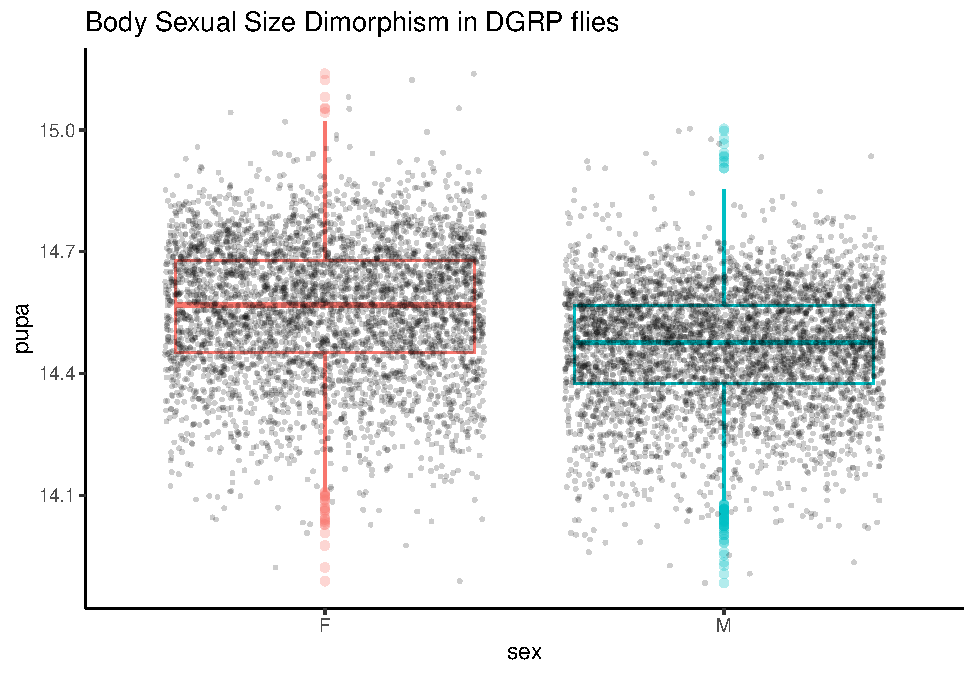
\includegraphics{_PreliminaryAnalysis_files/figure-latex/unnamed-chunk-8-1.pdf}

Answer 1.1: Yes, there is sexual size dimorphism in the DGRP flies, and
females are larger than males on average.

\hypertarget{question-1.2-do-we-see-a-genetic-variation-of-ssd-in-the-dgrp-lines}{%
\subsection{Question 1.2: Do we see a genetic variation of SSD in the
DGRP
lines?}\label{question-1.2-do-we-see-a-genetic-variation-of-ssd-in-the-dgrp-lines}}

\hypertarget{comparing-two-models-using-anova}{%
\subsubsection{Comparing two models using
ANOVA}\label{comparing-two-models-using-anova}}

\begin{Shaded}
\begin{Highlighting}[]
\CommentTok{#comparing two models}
\NormalTok{model2<-}\KeywordTok{lmer}\NormalTok{(pupa}\OperatorTok{~}\NormalTok{sex}\OperatorTok{+}\NormalTok{(}\DecValTok{1}\OperatorTok{|}\NormalTok{line)}\OperatorTok{+}\NormalTok{(}\DecValTok{1}\OperatorTok{|}\NormalTok{block), }\DataTypeTok{data=}\NormalTok{df0)  }\CommentTok{#model to test for SSD presence as we did above}
\NormalTok{model1<-}\KeywordTok{lmer}\NormalTok{(pupa}\OperatorTok{~}\NormalTok{sex}\OperatorTok{+}\NormalTok{(sex}\OperatorTok{|}\NormalTok{line)}\OperatorTok{+}\NormalTok{(}\DecValTok{1}\OperatorTok{|}\NormalTok{block), }\DataTypeTok{data=}\NormalTok{df0) }
\KeywordTok{anova}\NormalTok{(model1)}
\end{Highlighting}
\end{Shaded}

\begin{verbatim}
## Type III Analysis of Variance Table with Satterthwaite's method
##     Sum Sq Mean Sq NumDF  DenDF F value    Pr(>F)    
## sex 9.6134  9.6134     1 151.31  734.22 < 2.2e-16 ***
## ---
## Signif. codes:  0 '***' 0.001 '**' 0.01 '*' 0.05 '.' 0.1 ' ' 1
\end{verbatim}

\begin{Shaded}
\begin{Highlighting}[]
\KeywordTok{anova}\NormalTok{(model1,model2)}
\end{Highlighting}
\end{Shaded}

\begin{verbatim}
## Data: df0
## Models:
## model2: pupa ~ sex + (1 | line) + (1 | block)
## model1: pupa ~ sex + (sex | line) + (1 | block)
##        npar    AIC    BIC logLik deviance  Chisq Df Pr(>Chisq)    
## model2    5 -11285 -11250 5647.3   -11295                         
## model1    7 -11316 -11267 5664.9   -11330 35.264  2    2.2e-08 ***
## ---
## Signif. codes:  0 '***' 0.001 '**' 0.01 '*' 0.05 '.' 0.1 ' ' 1
\end{verbatim}

Model 1 is better, as AIC and BIC is smaller and log likelihood is
higher. The difference of fit between these two models is significant.

\hypertarget{do-a-lrt}{%
\subsubsection{Do a LRT}\label{do-a-lrt}}

How many parameters for each models

\begin{Shaded}
\begin{Highlighting}[]
\NormalTok{(}\KeywordTok{AIC}\NormalTok{(model1) }\OperatorTok{-}\StringTok{ }\KeywordTok{REMLcrit}\NormalTok{(model1))}\OperatorTok{/}\DecValTok{2} \CommentTok{# # of parameters the model "thinks" are being estimated}
\end{Highlighting}
\end{Shaded}

\begin{verbatim}
## [1] 7
\end{verbatim}

\begin{Shaded}
\begin{Highlighting}[]
\NormalTok{(}\KeywordTok{AIC}\NormalTok{(model2) }\OperatorTok{-}\StringTok{ }\KeywordTok{REMLcrit}\NormalTok{(model2))}\OperatorTok{/}\DecValTok{2} \CommentTok{# # of parameters the model "thinks" are being estimated}
\end{Highlighting}
\end{Shaded}

\begin{verbatim}
## [1] 5
\end{verbatim}

So lme4/lmer is treating model 1 as having two more parameters than
model2.

\begin{Shaded}
\begin{Highlighting}[]
\NormalTok{LR.model <-}\StringTok{  }\OperatorTok{-}\KeywordTok{as.numeric}\NormalTok{(}\KeywordTok{REMLcrit}\NormalTok{(model1) }\OperatorTok{-}\StringTok{ }\KeywordTok{REMLcrit}\NormalTok{(model2))}
\NormalTok{LR.model}
\end{Highlighting}
\end{Shaded}

\begin{verbatim}
## [1] 35.79724
\end{verbatim}

\begin{Shaded}
\begin{Highlighting}[]
\KeywordTok{nlevels}\NormalTok{(df}\OperatorTok{$}\NormalTok{line)}
\end{Highlighting}
\end{Shaded}

\begin{verbatim}
## [1] 0
\end{verbatim}

\begin{Shaded}
\begin{Highlighting}[]
\KeywordTok{pchisq}\NormalTok{(}\DataTypeTok{q =}\NormalTok{ LR.model, }\DataTypeTok{df=}\DecValTok{2}\NormalTok{, }\DataTypeTok{lower=}\NormalTok{F)}
\end{Highlighting}
\end{Shaded}

\begin{verbatim}
## [1] 1.685498e-08
\end{verbatim}

\begin{Shaded}
\begin{Highlighting}[]
\KeywordTok{pchisq}\NormalTok{(}\DataTypeTok{q =}\NormalTok{ LR.model, }\DataTypeTok{df=}\KeywordTok{nlevels}\NormalTok{(df}\OperatorTok{$}\NormalTok{line), }\DataTypeTok{lower=}\NormalTok{F)}
\end{Highlighting}
\end{Shaded}

\begin{verbatim}
## [1] 0
\end{verbatim}

\hypertarget{parametric-boostrap}{%
\subsubsection{Parametric boostrap}\label{parametric-boostrap}}

Finally, we can conduct a parametric bootstrap to compare the two
models.

\hypertarget{finally-using-bayesian-analysis}{%
\subsubsection{Finally using Bayesian
Analysis}\label{finally-using-bayesian-analysis}}

\begin{Shaded}
\begin{Highlighting}[]
\NormalTok{prior}\FloatTok{.2}\NormalTok{ <-}\KeywordTok{list}\NormalTok{(}\DataTypeTok{R=}\KeywordTok{list}\NormalTok{(}\DataTypeTok{V=}\FloatTok{0.01}\NormalTok{, }\DataTypeTok{nu=}\FloatTok{0.002}\NormalTok{), }
               \DataTypeTok{G=}\KeywordTok{list}\NormalTok{(}\DataTypeTok{G1=}\KeywordTok{list}\NormalTok{(}\DataTypeTok{V=}\FloatTok{0.01}\OperatorTok{*}\KeywordTok{diag}\NormalTok{(}\DecValTok{1}\NormalTok{), }\DataTypeTok{nu=}\FloatTok{0.002}\NormalTok{),}
                      \DataTypeTok{G2=}\KeywordTok{list}\NormalTok{(}\DataTypeTok{V=}\FloatTok{0.01}\OperatorTok{*}\KeywordTok{diag}\NormalTok{(}\DecValTok{2}\NormalTok{), }\DataTypeTok{nu=}\FloatTok{0.002}\NormalTok{)))}

\NormalTok{model1M.MCMC <-}\StringTok{ }\KeywordTok{MCMCglmm}\NormalTok{(pupa }\OperatorTok{~}\StringTok{ }\DecValTok{1} \OperatorTok{+}\StringTok{ }\NormalTok{sex, }
  \DataTypeTok{random=}\OperatorTok{~}\NormalTok{block }\OperatorTok{+}\StringTok{ }\KeywordTok{us}\NormalTok{(}\DecValTok{1} \OperatorTok{+}\StringTok{ }\NormalTok{sex)}\OperatorTok{:}\NormalTok{line,}
  \DataTypeTok{prior =}\NormalTok{ prior}\FloatTok{.2}\NormalTok{, }\DataTypeTok{burnin =} \DecValTok{5000}\NormalTok{, }\DataTypeTok{nitt =} \DecValTok{20000}\NormalTok{, }\DataTypeTok{thin =} \DecValTok{10}\NormalTok{,}
  \DataTypeTok{verbose =}\NormalTok{ F, }\DataTypeTok{pr =}\NormalTok{ T,}
  \DataTypeTok{data=}\NormalTok{df0)}
\KeywordTok{summary}\NormalTok{(model1M.MCMC)}
\end{Highlighting}
\end{Shaded}

\begin{verbatim}
## 
##  Iterations = 5001:19991
##  Thinning interval  = 10
##  Sample size  = 1500 
## 
##  DIC: -11819.27 
## 
##  G-structure:  ~block
## 
##       post.mean  l-95% CI u-95% CI eff.samp
## block  0.002842 0.0005402 0.006326     1500
## 
##                ~us(1 + sex):line
## 
##                               post.mean   l-95% CI   u-95% CI eff.samp
## (Intercept):(Intercept).line  0.0112904  0.0088854  0.0137445   1500.0
## sexM:(Intercept).line        -0.0013770 -0.0021987 -0.0005731   1277.1
## (Intercept):sexM.line        -0.0013770 -0.0021987 -0.0005731   1277.1
## sexM:sexM.line                0.0008693  0.0004248  0.0014007    709.1
## 
##  R-structure:  ~units
## 
##       post.mean l-95% CI u-95% CI eff.samp
## units   0.01311   0.0127   0.0135     1500
## 
##  Location effects: pupa ~ 1 + sex 
## 
##             post.mean l-95% CI u-95% CI eff.samp  pMCMC    
## (Intercept)  14.56336 14.52762 14.60167     1436 <7e-04 ***
## sexM         -0.09437 -0.10049 -0.08761     1500 <7e-04 ***
## ---
## Signif. codes:  0 '***' 0.001 '**' 0.01 '*' 0.05 '.' 0.1 ' ' 1
\end{verbatim}

\hypertarget{post-model-1-fitting-check}{%
\subsubsection{Post model 1 fitting
check}\label{post-model-1-fitting-check}}

\hypertarget{residual-distribution}{%
\paragraph{Residual distribution}\label{residual-distribution}}

\begin{Shaded}
\begin{Highlighting}[]
\NormalTok{res_model1=}\KeywordTok{residuals}\NormalTok{(model1)}
\end{Highlighting}
\end{Shaded}

\hypertarget{model-1-residual-distribution}{%
\paragraph{Model 1 residual
distribution}\label{model-1-residual-distribution}}

\begin{Shaded}
\begin{Highlighting}[]
\KeywordTok{plot}\NormalTok{(model1)}
\end{Highlighting}
\end{Shaded}

\includegraphics{_PreliminaryAnalysis_files/figure-latex/unnamed-chunk-15-1.pdf}

\hypertarget{qq-plot}{%
\paragraph{QQ plot}\label{qq-plot}}

\begin{Shaded}
\begin{Highlighting}[]
\KeywordTok{require}\NormalTok{(ggpubr)}
\KeywordTok{ggqqplot}\NormalTok{(res_model1)}
\end{Highlighting}
\end{Shaded}

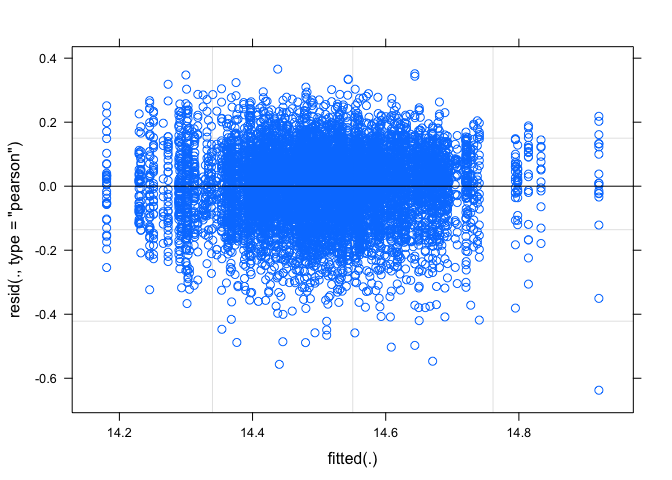
\includegraphics{_PreliminaryAnalysis_files/figure-latex/unnamed-chunk-16-1.pdf}

\hypertarget{random-effect-plot}{%
\paragraph{Random effect plot}\label{random-effect-plot}}

\begin{Shaded}
\begin{Highlighting}[]
\KeywordTok{qqmath}\NormalTok{(}\KeywordTok{ranef}\NormalTok{(model1))}
\end{Highlighting}
\end{Shaded}

\begin{verbatim}
## $line
\end{verbatim}

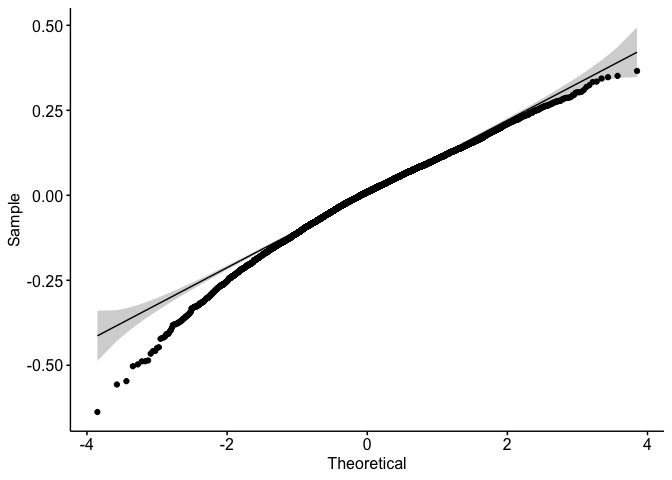
\includegraphics{_PreliminaryAnalysis_files/figure-latex/unnamed-chunk-17-1.pdf}

\begin{verbatim}
## 
## $block
\end{verbatim}

\includegraphics{_PreliminaryAnalysis_files/figure-latex/unnamed-chunk-17-2.pdf}
We have two plots, one for line and one for block

\hypertarget{question-1.3-is-ssd-genetic-variation-due-to-the-genetic-variation-in-male-or-in-female-size}{%
\subsection{Question 1.3: Is SSD genetic variation due to the genetic
variation in male or in female
size?}\label{question-1.3-is-ssd-genetic-variation-due-to-the-genetic-variation-in-male-or-in-female-size}}

To test this, I need to look at the correlation between SSD and male
size and SSD and female size, the correlation that is higher means that
that sex contributes the most to the SSD variation.

I need to calculate summary for pupa female size, pupa male size and
SSD.

\begin{Shaded}
\begin{Highlighting}[]
\CommentTok{#calculate means for each group using pupa_noblock}
\KeywordTok{head}\NormalTok{(df0)}
\end{Highlighting}
\end{Shaded}

\begin{verbatim}
## # A tibble: 6 x 10
## # Groups:   group [6]
##   id             line  block day   sex    wing   leg  pupa group    pupa_noblock
##   <chr>          <chr> <chr> <chr> <chr> <dbl> <dbl> <dbl> <chr>           <dbl>
## 1 853-A-0-M-027  L853  B7    D0    M      13.9  13.9  13.9 L853_M_~       -0.485
## 2 317-B-0-F-6693 L317  B11   D0    F      13.8  13.6  13.9 L317_F_~       -0.536
## 3 787-A-0-M-011  L787  B7    D0    M      13.9  13.6  13.9 L787_M_~       -0.462
## 4 513-B-0-F-59   L513  B13   D0    F      13.4  13.1  13.9 L513_F_~       -0.532
## 5 513-B-0-M-61   L513  B13   D0    M      13.4  13.2  13.9 L513_M_~       -0.527
## 6 492-A-0-M-014  L492  B6    D0    M      13.4  13.2  13.9 L492_M_~       -0.437
\end{verbatim}

\begin{Shaded}
\begin{Highlighting}[]
\NormalTok{df0_mean<-}\KeywordTok{aggregate}\NormalTok{(df0[, }\DecValTok{10}\NormalTok{], }\KeywordTok{list}\NormalTok{(df0}\OperatorTok{$}\NormalTok{group), mean)}
\KeywordTok{head}\NormalTok{(df0_mean)}
\end{Highlighting}
\end{Shaded}

\begin{verbatim}
##     Group.1 pupa_noblock
## 1 L100_F_D0  0.256259113
## 2 L100_M_D0  0.117684442
## 3 L101_F_D0  0.109003255
## 4 L101_M_D0  0.089615441
## 5 L105_F_D0 -0.003621951
## 6 L105_M_D0 -0.053412213
\end{verbatim}

\begin{Shaded}
\begin{Highlighting}[]
\CommentTok{#re-add line, day and sex columns}
\NormalTok{df0_mean<-df0_mean }\OperatorTok
\StringTok{  }\KeywordTok{separate}\NormalTok{(Group}\FloatTok{.1}\NormalTok{, }\KeywordTok{c}\NormalTok{(}\StringTok{"line"}\NormalTok{, }\StringTok{"sex"}\NormalTok{,}\StringTok{"day"}\NormalTok{), }\StringTok{"_"}\NormalTok{)}
\KeywordTok{head}\NormalTok{(df0_mean)}
\end{Highlighting}
\end{Shaded}

\begin{verbatim}
##   line sex day pupa_noblock
## 1 L100   F  D0  0.256259113
## 2 L100   M  D0  0.117684442
## 3 L101   F  D0  0.109003255
## 4 L101   M  D0  0.089615441
## 5 L105   F  D0 -0.003621951
## 6 L105   M  D0 -0.053412213
\end{verbatim}

\begin{Shaded}
\begin{Highlighting}[]
\NormalTok{df0_mean}
\end{Highlighting}
\end{Shaded}

\begin{verbatim}
##     line sex day  pupa_noblock
## 1   L100   F  D0  0.2562591132
## 2   L100   M  D0  0.1176844420
## 3   L101   F  D0  0.1090032548
## 4   L101   M  D0  0.0896154415
## 5   L105   F  D0 -0.0036219507
## 6   L105   M  D0 -0.0534122128
## 7   L109   F  D0  0.0631802323
## 8   L109   M  D0 -0.0201975436
## 9   L136   F  D0  0.1843059842
## 10  L136   M  D0  0.0686724726
## 11  L138   F  D0  0.2072351018
## 12  L138   M  D0  0.1205746724
## 13  L142   F  D0  0.3154994151
## 14  L142   M  D0  0.1862461902
## 15  L149   F  D0  0.2939633932
## 16  L149   M  D0  0.2263605352
## 17  L153   M  D0  0.1720938761
## 18  L158   F  D0  0.4372960793
## 19  L158   M  D0  0.2932614485
## 20  L161   F  D0  0.0532078641
## 21  L161   M  D0 -0.0798339088
## 22  L176   F  D0  0.1077974775
## 23  L176   M  D0  0.0598671462
## 24  L177   F  D0  0.0993704618
## 25  L177   M  D0 -0.0249945976
## 26  L181   F  D0  0.1185554791
## 27  L181   M  D0  0.0217470498
## 28  L189   F  D0  0.1460412682
## 29  L189   M  D0  0.0899009209
## 30  L195   F  D0  0.2585795499
## 31  L195   M  D0  0.1081613901
## 32  L208   F  D0  0.1022639809
## 33  L208   M  D0  0.0246569663
## 34   L21   F  D0  0.0840488460
## 35   L21   M  D0  0.1678136089
## 36  L217   F  D0  0.1476354697
## 37  L217   M  D0  0.0616153638
## 38  L227   F  D0  0.3046909187
## 39  L227   M  D0  0.1373850570
## 40  L228   F  D0  0.0753968955
## 41  L228   M  D0 -0.0563289145
## 42  L229   F  D0  0.2342913759
## 43  L229   M  D0  0.1029741681
## 44  L235   F  D0 -0.1270181905
## 45  L235   M  D0 -0.1425841151
## 46  L237   F  D0  0.2055254217
## 47  L237   M  D0  0.0327023053
## 48  L239   F  D0  0.0056334871
## 49  L239   M  D0  0.0081306941
## 50  L256   F  D0  0.1506148709
## 51  L256   M  D0  0.0905072026
## 52   L26   F  D0  0.2132552383
## 53   L26   M  D0  0.1038144443
## 54   L28   F  D0  0.2039807619
## 55   L28   M  D0  0.1450800836
## 56  L287   F  D0  0.1983714164
## 57  L287   M  D0  0.1166650745
## 58  L303   F  D0  0.1840538837
## 59  L303   M  D0  0.1269183963
## 60  L306   F  D0  0.3359031160
## 61  L306   M  D0  0.2165760477
## 62  L307   F  D0  0.2268676891
## 63  L307   M  D0  0.1129487001
## 64  L309   F  D0  0.2571231521
## 65  L309   M  D0  0.1357655568
## 66   L31   F  D0  0.2456848272
## 67   L31   M  D0  0.1008883367
## 68  L313   F  D0  0.0864244932
## 69  L313   M  D0 -0.0023952978
## 70  L315   F  D0  0.3029378471
## 71  L315   M  D0  0.1455292296
## 72  L317   F  D0 -0.0515839558
## 73  L317   M  D0 -0.1484657346
## 74  L318   F  D0  0.1696493109
## 75  L318   M  D0  0.0504898756
## 76  L319   F  D0  0.1785986230
## 77  L319   M  D0  0.0906516737
## 78   L32   F  D0  0.1129675992
## 79   L32   M  D0 -0.0311321817
## 80  L320   F  D0  0.1848466510
## 81  L320   M  D0  0.0788483577
## 82  L321   F  D0  0.0808203321
## 83  L321   M  D0 -0.0561055658
## 84  L324   F  D0  0.2364513085
## 85  L324   M  D0  0.1004870022
## 86  L332   F  D0  0.0155957763
## 87  L332   M  D0 -0.0534027131
## 88  L335   F  D0 -0.0307045241
## 89  L335   M  D0 -0.1805070078
## 90  L336   F  D0  0.0967968694
## 91  L336   M  D0 -0.0362019647
## 92  L338   F  D0  0.1523652135
## 93  L338   M  D0  0.0882672765
## 94  L340   F  D0  0.2300307638
## 95  L340   M  D0  0.1605795608
## 96  L348   F  D0  0.1993774319
## 97  L348   M  D0  0.0232363355
## 98  L350   F  D0  0.1480021833
## 99  L350   M  D0 -0.0387438220
## 100 L352   F  D0  0.0487995777
## 101 L352   M  D0 -0.0378955926
## 102 L354   F  D0  0.1098169623
## 103 L354   M  D0  0.0051935203
## 104 L356   F  D0  0.1317035726
## 105 L356   M  D0  0.0004412101
## 106 L357   F  D0  0.1708191014
## 107 L357   M  D0  0.0724084958
## 108 L358   F  D0  0.0414353058
## 109 L358   M  D0 -0.0523739437
## 110 L359   F  D0  0.1570596863
## 111 L359   M  D0  0.1178283189
## 112 L360   F  D0  0.2006730866
## 113 L360   M  D0  0.1656891299
## 114 L361   F  D0  0.0135541493
## 115 L361   M  D0 -0.0885247499
## 116 L362   F  D0  0.1732051217
## 117 L362   M  D0  0.0122061209
## 118 L365   F  D0  0.1642452047
## 119 L365   M  D0  0.0291681632
## 120 L367   F  D0  0.2181460221
## 121 L367   M  D0  0.1237970900
## 122 L370   F  D0 -0.1081694750
## 123 L370   M  D0 -0.0663318156
## 124 L371   F  D0  0.1845707343
## 125 L371   M  D0  0.0481868765
## 126 L373   F  D0  0.0851325537
## 127 L373   M  D0 -0.0803733426
## 128 L374   F  D0  0.0012177485
## 129 L374   M  D0 -0.0555312838
## 130 L375   F  D0  0.0400445338
## 131 L375   M  D0 -0.0324891968
## 132 L377   M  D0  0.0474887028
## 133 L379   F  D0  0.1693221236
## 134 L379   M  D0  0.1424013423
## 135  L38   F  D0  0.1020119932
## 136  L38   M  D0  0.0320820370
## 137 L380   F  D0  0.1683659260
## 138 L380   M  D0  0.0944210463
## 139 L381   F  D0  0.0028879795
## 140 L381   M  D0 -0.0195703267
## 141 L383   F  D0  0.2673719701
## 142 L383   M  D0  0.0952737430
## 143 L385   F  D0  0.1910376523
## 144 L385   M  D0  0.0849628594
## 145 L386   F  D0  0.1445082928
## 146 L386   M  D0  0.0586189416
## 147 L390   F  D0  0.1903807011
## 148 L390   M  D0  0.0934446239
## 149 L391   F  D0  0.1959914642
## 150 L391   M  D0  0.1011750908
## 151 L392   F  D0  0.2825889438
## 152 L392   M  D0  0.1635001128
## 153 L395   F  D0  0.1203233909
## 154 L395   M  D0  0.1662620706
## 155 L397   F  D0  0.1010190402
## 156 L397   M  D0  0.0534231558
## 157 L399   F  D0  0.2291997204
## 158 L399   M  D0  0.1517342230
## 159 L405   F  D0  0.0947842632
## 160 L405   M  D0  0.0382211162
## 161 L406   F  D0  0.2385650575
## 162 L406   M  D0  0.1192671587
## 163 L409   F  D0  0.3014213915
## 164 L409   M  D0  0.1614964351
## 165  L41   F  D0  0.0322932535
## 166  L41   M  D0 -0.0922310834
## 167  L42   F  D0  0.2368225169
## 168  L42   M  D0  0.1245236872
## 169 L426   F  D0  0.0501950637
## 170 L426   M  D0 -0.0538399401
## 171 L427   F  D0  0.1260385199
## 172 L427   M  D0  0.0421587020
## 173 L437   F  D0  0.1320315268
## 174 L437   M  D0  0.0629462657
## 175 L439   F  D0 -0.0943645732
## 176 L439   M  D0 -0.0822292307
## 177 L440   F  D0  0.1341472997
## 178 L440   M  D0  0.0287374373
## 179 L441   F  D0  0.1418139705
## 180 L441   M  D0  0.0805356803
## 181 L443   F  D0  0.2731604922
## 182 L443   M  D0  0.1622909259
## 183  L45   F  D0 -0.0585724792
## 184  L45   M  D0 -0.1559471493
## 185 L461   F  D0  0.1117271324
## 186 L461   M  D0 -0.0735474853
## 187 L486   F  D0  0.0537211857
## 188 L486   M  D0  0.0336351322
## 189 L491   F  D0  0.0030675732
## 190 L491   M  D0 -0.0629334823
## 191 L492   F  D0  0.0520489428
## 192 L492   M  D0 -0.1009464177
## 193 L502   F  D0  0.1553739158
## 194 L502   M  D0  0.0231500349
## 195 L505   F  D0  0.1525335362
## 196 L505   M  D0  0.0665868515
## 197 L508   F  D0  0.0668807856
## 198 L508   M  D0  0.0239739135
## 199 L509   F  D0  0.4012180659
## 200 L509   M  D0  0.2746670093
## 201 L513   F  D0 -0.2029003501
## 202 L513   M  D0 -0.2722340895
## 203 L517   F  D0  0.0995945691
## 204 L517   M  D0 -0.0026889697
## 205 L528   F  D0  0.0942672005
## 206 L528   M  D0 -0.0030951674
## 207 L530   F  D0  0.2064055617
## 208 L530   M  D0  0.0377337408
## 209 L531   F  D0  0.2990803387
## 210 L531   M  D0  0.1789519213
## 211 L535   F  D0  0.1325805707
## 212 L535   M  D0  0.0406165075
## 213 L551   F  D0  0.2346518923
## 214 L551   M  D0  0.0807640141
## 215 L555   F  D0  0.2419390191
## 216 L555   M  D0  0.0792034266
## 217 L559   M  D0  0.0527739182
## 218 L563   F  D0  0.1038066797
## 219 L563   M  D0  0.0014342731
## 220 L566   F  D0  0.1281033667
## 221 L566   M  D0  0.0612490537
## 222  L57   F  D0 -0.0006133461
## 223  L57   M  D0 -0.1346996293
## 224 L589   F  D0  0.1176607444
## 225 L589   M  D0 -0.0100653228
## 226  L59   F  D0  0.0985270542
## 227  L59   M  D0  0.0109984238
## 228 L595   F  D0  0.0299226181
## 229 L595   M  D0 -0.0677586404
## 230 L596   F  D0  0.0660390305
## 231 L596   M  D0 -0.0721477471
## 232 L627   F  D0  0.1044915504
## 233 L627   M  D0  0.1794276743
## 234 L630   F  D0  0.1658963323
## 235 L630   M  D0  0.0963656978
## 236 L634   M  D0  0.0806280071
## 237 L639   F  D0  0.1566195853
## 238 L639   M  D0  0.0639985807
## 239 L646   F  D0  0.0871639538
## 240 L646   M  D0  0.0269296473
## 241  L69   F  D0  0.1841270081
## 242  L69   M  D0 -0.0141390825
## 243 L703   F  D0  0.0136949361
## 244 L703   M  D0 -0.0815453571
## 245 L705   F  D0  0.2573151269
## 246 L705   M  D0  0.1631921017
## 247 L707   F  D0  0.2334951428
## 248 L707   M  D0  0.0893997695
## 249 L712   F  D0 -0.0113711624
## 250 L712   M  D0 -0.0710397043
## 251 L714   F  D0  0.2711197887
## 252 L714   M  D0  0.1478309594
## 253 L716   F  D0  0.1515912202
## 254 L716   M  D0  0.0963159732
## 255 L721   F  D0  0.0612395963
## 256 L721   M  D0 -0.1035635424
## 257 L727   F  D0  0.2046712967
## 258 L727   M  D0  0.0951000719
## 259  L73   F  D0  0.0609073463
## 260  L73   M  D0  0.0613024336
## 261 L730   F  D0  0.2727569732
## 262 L730   M  D0  0.1650894655
## 263 L732   F  D0  0.1848820530
## 264 L732   M  D0  0.0473187380
## 265 L737   F  D0  0.2536484601
## 266 L737   M  D0  0.1066902166
## 267 L738   F  D0  0.1424360647
## 268 L738   M  D0  0.1258668146
## 269 L748   F  D0  0.1786037049
## 270 L748   M  D0  0.0727599492
## 271  L75   F  D0  0.1107145983
## 272  L75   M  D0  0.0403227352
## 273 L757   F  D0  0.2343497444
## 274 L757   M  D0  0.0483669070
## 275 L761   F  D0  0.0606307493
## 276 L761   M  D0  0.0450327392
## 277 L765   F  D0 -0.0669197107
## 278 L765   M  D0 -0.1002547860
## 279 L774   F  D0  0.0631625520
## 280 L774   M  D0 -0.0683610287
## 281 L776   F  D0  0.2081936743
## 282 L776   M  D0  0.0606021859
## 283 L783   F  D0  0.2127960628
## 284 L783   M  D0  0.1399479996
## 285 L786   F  D0  0.0690268670
## 286 L786   M  D0 -0.0410587856
## 287 L787   F  D0  0.0636893689
## 288 L787   M  D0 -0.0151044233
## 289 L790   F  D0  0.0727080353
## 290 L790   M  D0  0.0247763017
## 291 L796   F  D0 -0.0206491805
## 292 L796   M  D0 -0.0552568930
## 293 L799   F  D0  0.1319339348
## 294 L799   M  D0  0.1130388579
## 295 L801   F  D0  0.1122320206
## 296 L801   M  D0  0.0162623618
## 297 L802   F  D0  0.3379647865
## 298 L802   M  D0  0.2479234838
## 299 L805   F  D0  0.1394454026
## 300 L805   M  D0  0.0550037917
## 301 L808   F  D0  0.2164807601
## 302 L808   M  D0  0.1038783140
## 303 L810   F  D0  0.3138488117
## 304 L810   M  D0  0.2122877194
## 305 L812   F  D0  0.4460601241
## 306 L812   M  D0  0.3653371591
## 307 L818   F  D0  0.1065008293
## 308 L818   M  D0  0.0085809252
## 309 L819   F  D0 -0.0369446409
## 310 L819   M  D0 -0.1052705482
## 311 L821   F  D0  0.1271722303
## 312 L821   M  D0  0.0453121285
## 313 L822   F  D0  0.1834076229
## 314 L822   M  D0  0.1359787966
## 315  L83   F  D0  0.0559405653
## 316  L83   M  D0 -0.0018613695
## 317 L832   F  D0  0.2486188891
## 318 L832   M  D0  0.1918970172
## 319 L837   F  D0  0.0559750010
## 320 L837   M  D0 -0.0176497124
## 321 L843   F  D0  0.0830188158
## 322 L843   M  D0 -0.0176519357
## 323 L849   F  D0  0.0394450449
## 324 L849   M  D0  0.0955541856
## 325  L85   F  D0  0.2599100116
## 326  L85   M  D0  0.0932143968
## 327 L850   F  D0  0.0970174922
## 328 L850   M  D0  0.0541179849
## 329 L852   F  D0  0.2817583766
## 330 L852   M  D0  0.0506834321
## 331 L853   F  D0  0.1528419804
## 332 L853   M  D0  0.0794362396
## 333 L855   F  D0  0.0526886849
## 334 L855   M  D0 -0.0445882945
## 335 L857   F  D0  0.1590773049
## 336 L857   M  D0  0.0914103924
## 337 L859   F  D0  0.3334562328
## 338 L859   M  D0  0.1761790132
## 339 L861   F  D0 -0.0187212383
## 340 L861   M  D0 -0.0928993254
## 341  L88   F  D0 -0.0767957270
## 342  L88   M  D0 -0.1659863989
## 343 L882   F  D0  0.1030156141
## 344 L882   M  D0  0.0504505732
## 345 L884   F  D0  0.0265367112
## 346 L884   M  D0  0.0234148809
## 347 L887   F  D0 -0.0941412019
## 348 L887   M  D0 -0.1739419358
## 349 L890   F  D0  0.2499141394
## 350 L890   M  D0  0.1176510268
## 351 L892   F  D0  0.1478955704
## 352 L892   M  D0  0.1213591580
## 353 L894   F  D0  0.2052807366
## 354 L894   M  D0  0.1086813376
## 355 L897   F  D0  0.0822568587
## 356 L897   M  D0  0.0037052421
## 357 L900   F  D0  0.1334762105
## 358 L900   M  D0  0.0222409081
## 359 L907   F  D0  0.3240363799
## 360 L907   M  D0  0.1775240544
## 361 L908   F  D0  0.0559346136
## 362 L908   M  D0 -0.1042680943
## 363  L91   F  D0  0.2777092445
## 364  L91   M  D0  0.1355913376
## 365 L911   F  D0 -0.0932964914
## 366 L911   M  D0 -0.1239980597
## 367 L913   M  D0  0.0643726760
## 368  L93   F  D0  0.3018310838
## 369  L93   M  D0  0.1884805791
\end{verbatim}

Size Mean by line plot boxplot for fed flies

\begin{Shaded}
\begin{Highlighting}[]
\CommentTok{# this plot is based on the variation excluding block effect}
\KeywordTok{head}\NormalTok{(df0_mean)}
\end{Highlighting}
\end{Shaded}

\begin{verbatim}
##   line sex day pupa_noblock
## 1 L100   F  D0  0.256259113
## 2 L100   M  D0  0.117684442
## 3 L101   F  D0  0.109003255
## 4 L101   M  D0  0.089615441
## 5 L105   F  D0 -0.003621951
## 6 L105   M  D0 -0.053412213
\end{verbatim}

\begin{Shaded}
\begin{Highlighting}[]
\NormalTok{df0_mean }\OperatorTok
\StringTok{  }\KeywordTok{ggplot}\NormalTok{(}\KeywordTok{aes}\NormalTok{(sex,pupa_noblock, }\DataTypeTok{fill=}\NormalTok{sex)) }\OperatorTok{+}
\StringTok{  }\KeywordTok{geom_boxplot}\NormalTok{() }\OperatorTok{+}
\StringTok{  }\KeywordTok{geom_point}\NormalTok{(}\DataTypeTok{size=}\FloatTok{0.5}\NormalTok{)}\OperatorTok{+}\StringTok{ }
\StringTok{  }\KeywordTok{geom_line}\NormalTok{(}\KeywordTok{aes}\NormalTok{(}\DataTypeTok{group=}\NormalTok{line, }\DataTypeTok{alpha=}\FloatTok{0.1}\NormalTok{, }\DataTypeTok{linewidth=}\FloatTok{0.5}\NormalTok{)) }\OperatorTok{+}
\StringTok{  }\KeywordTok{theme}\NormalTok{(}\DataTypeTok{legend.position =} \StringTok{"none"}\NormalTok{)}
\end{Highlighting}
\end{Shaded}

\begin{verbatim}
## Warning: Ignoring unknown aesthetics: linewidth
\end{verbatim}

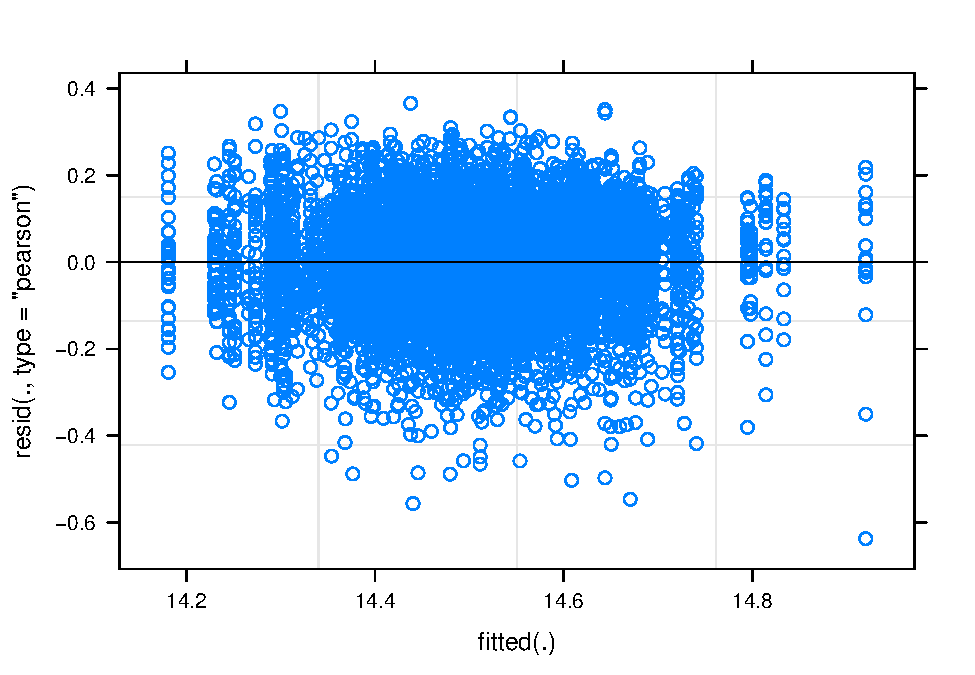
\includegraphics{_PreliminaryAnalysis_files/figure-latex/unnamed-chunk-19-1.pdf}

\begin{Shaded}
\begin{Highlighting}[]
\CommentTok{#calculate SSD0}
\CommentTok{#separating males and females to put the values in columns}
\NormalTok{df0_mean_F<-}\KeywordTok{subset}\NormalTok{(df0_mean, sex}\OperatorTok{==}\StringTok{"F"}\NormalTok{)}
\NormalTok{df0_mean_M<-}\KeywordTok{subset}\NormalTok{(df0_mean, sex}\OperatorTok{==}\StringTok{"M"}\NormalTok{)}

\NormalTok{df0_mean_}\DecValTok{2}\NormalTok{<-}\KeywordTok{merge}\NormalTok{(}\DataTypeTok{x=}\NormalTok{df0_mean_F, }\DataTypeTok{y=}\NormalTok{df0_mean_M, }\DataTypeTok{by.x=}\StringTok{"line"}\NormalTok{, }\DataTypeTok{by.y=}\StringTok{"line"}\NormalTok{)}
\KeywordTok{head}\NormalTok{(df0_mean_}\DecValTok{2}\NormalTok{)}
\end{Highlighting}
\end{Shaded}

\begin{verbatim}
##   line sex.x day.x pupa_noblock.x sex.y day.y pupa_noblock.y
## 1 L100     F    D0    0.256259113     M    D0     0.11768444
## 2 L101     F    D0    0.109003255     M    D0     0.08961544
## 3 L105     F    D0   -0.003621951     M    D0    -0.05341221
## 4 L109     F    D0    0.063180232     M    D0    -0.02019754
## 5 L136     F    D0    0.184305984     M    D0     0.06867247
## 6 L138     F    D0    0.207235102     M    D0     0.12057467
\end{verbatim}

\begin{Shaded}
\begin{Highlighting}[]
\CommentTok{#remove extra columns}
\NormalTok{df0_mean_}\DecValTok{2}\NormalTok{<-df0_mean_}\DecValTok{2}\NormalTok{[,}\KeywordTok{c}\NormalTok{(}\DecValTok{1}\NormalTok{,}\DecValTok{4}\NormalTok{,}\DecValTok{7}\NormalTok{)] }\CommentTok{#line, pupa_noblockF and pupa_noblockM}
\KeywordTok{colnames}\NormalTok{(df0_mean_}\DecValTok{2}\NormalTok{) <-}\StringTok{ }\KeywordTok{c}\NormalTok{(}\StringTok{"line"}\NormalTok{, }\StringTok{"pupaF"}\NormalTok{, }\StringTok{"pupaM"}\NormalTok{) }\CommentTok{#rename col}

\NormalTok{df0_mean<-df0_mean_}\DecValTok{2} \CommentTok{#move back to df0_mean}
\NormalTok{df0_mean}\OperatorTok{$}\NormalTok{SSD0<-}\StringTok{ }\NormalTok{df0_mean}\OperatorTok{$}\NormalTok{pupaF }\OperatorTok{-}\StringTok{ }\NormalTok{df0_mean}\OperatorTok{$}\NormalTok{pupaM  }\CommentTok{#since we established that females are larger than males in general, SSD is female-male sizes}
\KeywordTok{head}\NormalTok{(df0_mean) }\CommentTok{#182 lines}
\end{Highlighting}
\end{Shaded}

\begin{verbatim}
##   line        pupaF       pupaM       SSD0
## 1 L100  0.256259113  0.11768444 0.13857467
## 2 L101  0.109003255  0.08961544 0.01938781
## 3 L105 -0.003621951 -0.05341221 0.04979026
## 4 L109  0.063180232 -0.02019754 0.08337778
## 5 L136  0.184305984  0.06867247 0.11563351
## 6 L138  0.207235102  0.12057467 0.08666043
\end{verbatim}

Correlation test

\begin{Shaded}
\begin{Highlighting}[]
\KeywordTok{corr.test}\NormalTok{(df0_mean[}\DecValTok{2}\OperatorTok{:}\DecValTok{4}\NormalTok{],}
          \DataTypeTok{use    =} \StringTok{"pairwise"}\NormalTok{,}
          \DataTypeTok{method =} \StringTok{"pearson"}\NormalTok{,}
          \DataTypeTok{adjust =} \StringTok{"none"}\NormalTok{)}
\end{Highlighting}
\end{Shaded}

\begin{verbatim}
## Call:corr.test(x = df0_mean[2:4], use = "pairwise", method = "pearson", 
##     adjust = "none")
## Correlation matrix 
##       pupaF pupaM  SSD0
## pupaF  1.00  0.89  0.43
## pupaM  0.89  1.00 -0.04
## SSD0   0.43 -0.04  1.00
## Sample Size 
## [1] 182
## Probability values (Entries above the diagonal are adjusted for multiple tests.) 
##       pupaF pupaM SSD0
## pupaF     0  0.00 0.00
## pupaM     0  0.00 0.62
## SSD0      0  0.62 0.00
## 
##  To see confidence intervals of the correlations, print with the short=FALSE option
\end{verbatim}

\begin{Shaded}
\begin{Highlighting}[]
\KeywordTok{chart.Correlation}\NormalTok{(df0_mean[}\DecValTok{2}\OperatorTok{:}\DecValTok{4}\NormalTok{],}
                   \DataTypeTok{method=}\StringTok{"pearson"}\NormalTok{,}
                   \DataTypeTok{histogram=}\OtherTok{TRUE}\NormalTok{,}
                   \DataTypeTok{pch=}\DecValTok{16}\NormalTok{)}
\end{Highlighting}
\end{Shaded}

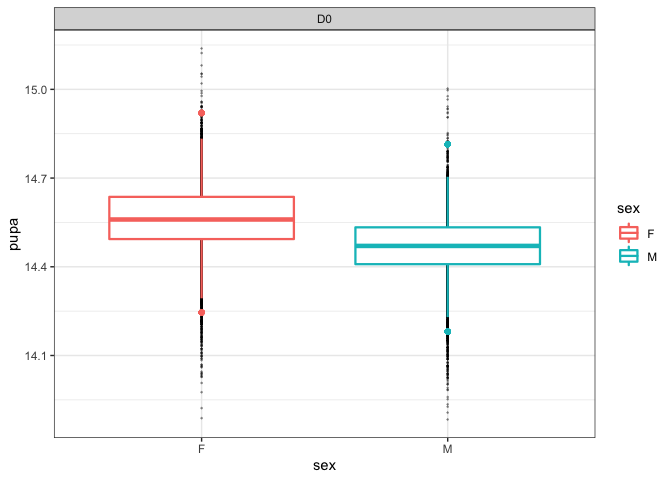
\includegraphics{_PreliminaryAnalysis_files/figure-latex/unnamed-chunk-22-1.pdf}
It seems that SSD in fed flies co-varies with the most with female size.
The R2 is not very high though, so it is not all that explains SSD0
variation.

Does female size vary more genetically than male size?

One tail variance F test

\begin{Shaded}
\begin{Highlighting}[]
\CommentTok{#Before performing the F test, I need to check that both samples are normally distributed.}
\KeywordTok{require}\NormalTok{(ggpubr)}
\KeywordTok{ggqqplot}\NormalTok{(df0_mean}\OperatorTok{$}\NormalTok{pupaF)}
\end{Highlighting}
\end{Shaded}

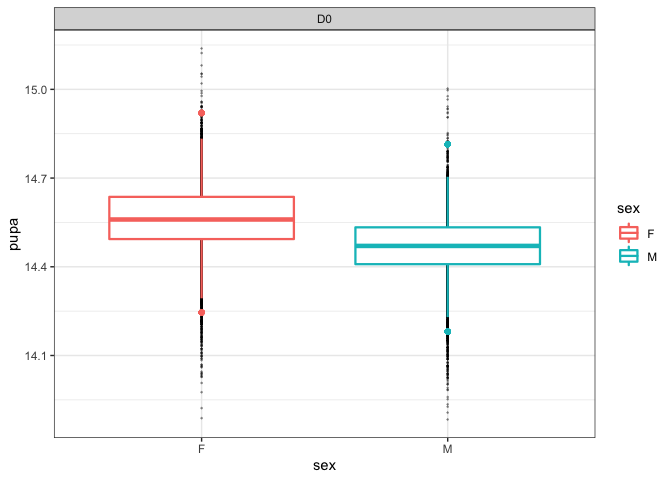
\includegraphics{_PreliminaryAnalysis_files/figure-latex/unnamed-chunk-23-1.pdf}

\begin{Shaded}
\begin{Highlighting}[]
\KeywordTok{ggqqplot}\NormalTok{(df0_mean}\OperatorTok{$}\NormalTok{pupaM)}
\end{Highlighting}
\end{Shaded}

\includegraphics{_PreliminaryAnalysis_files/figure-latex/unnamed-chunk-23-2.pdf}

\begin{Shaded}
\begin{Highlighting}[]
\KeywordTok{shapiro.test}\NormalTok{(df0_mean}\OperatorTok{$}\NormalTok{pupaM) }\CommentTok{#normal distribution}
\end{Highlighting}
\end{Shaded}

\begin{verbatim}
## 
##  Shapiro-Wilk normality test
## 
## data:  df0_mean$pupaM
## W = 0.99272, p-value = 0.4996
\end{verbatim}

\begin{Shaded}
\begin{Highlighting}[]
\KeywordTok{shapiro.test}\NormalTok{(df0_mean}\OperatorTok{$}\NormalTok{pupaF) }\CommentTok{#normal distribution}
\end{Highlighting}
\end{Shaded}

\begin{verbatim}
## 
##  Shapiro-Wilk normality test
## 
## data:  df0_mean$pupaF
## W = 0.99563, p-value = 0.8788
\end{verbatim}

\begin{Shaded}
\begin{Highlighting}[]
\CommentTok{#one tail F test}

\KeywordTok{var.test}\NormalTok{(df0_mean}\OperatorTok{$}\NormalTok{pupaF, df0_mean}\OperatorTok{$}\NormalTok{pupaM, }\DataTypeTok{alternative =} \StringTok{"greater"}\NormalTok{)}
\end{Highlighting}
\end{Shaded}

\begin{verbatim}
## 
##  F test to compare two variances
## 
## data:  df0_mean$pupaF and df0_mean$pupaM
## F = 1.2274, num df = 181, denom df = 181, p-value = 0.08453
## alternative hypothesis: true ratio of variances is greater than 1
## 95 percent confidence interval:
##  0.9605383       Inf
## sample estimates:
## ratio of variances 
##           1.227407
\end{verbatim}

The variance in female size is actually not larger than the variance in
male size, despite the higher correlation between female size and SSD0,
than male size and SS0. So does it mean that SSD0 varies partly because
of a co-variation with female size but not from the fact that female
size varies more genetically? So where does that SSD variation come
from?

\hypertarget{section-2-ssd-in-other-conditions}{%
\section{Section 2: SSD in other
conditions}\label{section-2-ssd-in-other-conditions}}

We found that in fed flies, females are on average larger than males, so
there is a female biased SSD. That SSD also vary genetically. We finally
found out that SSD variation is in part driven by the genetic variation
of female size, although the variance of female size is the same as male
size.

Let's look at different starving conditions

\begin{itemize}
\tightlist
\item
  Question 2.1: Do we have the same SSD when we change environment? NO
\item
  Question 2.2: Does SSD increase or decrease when the flies are
  starved? Our hypothesis is that overall SSD should decrease
\item
  Question 2.3: Does the SSD in starved conditions vary the same way as
  in fed flies?
\end{itemize}

\hypertarget{question-2.1-do-we-have-the-same-ssd-when-we-change-environment}{%
\subsection{Question 2.1: Do we have the same SSD when we change
environment?}\label{question-2.1-do-we-have-the-same-ssd-when-we-change-environment}}

\hypertarget{day-starvation-data}{%
\subsubsection{1 day starvation data}\label{day-starvation-data}}

\begin{Shaded}
\begin{Highlighting}[]
\CommentTok{#subset day 1 and day 2 starvation}

\CommentTok{#fisrt subset Day1 data from df_sub}
\NormalTok{df1<-}\KeywordTok{subset}\NormalTok{(df_sub, day}\OperatorTok{==}\StringTok{"D1"}\NormalTok{) }\CommentTok{#df_sub N<10 per group filtered out already}

\CommentTok{#na.omit only if pupa has NA}
\NormalTok{df1<-}\KeywordTok{na.omit}\NormalTok{(df1, }\DataTypeTok{cols=}\StringTok{"pupa"}\NormalTok{) }\CommentTok{#6409 rows}
\KeywordTok{length}\NormalTok{(}\KeywordTok{unique}\NormalTok{(df1}\OperatorTok{$}\NormalTok{line)) }\CommentTok{#179 lines left}
\end{Highlighting}
\end{Shaded}

\begin{verbatim}
## [1] 179
\end{verbatim}

\begin{Shaded}
\begin{Highlighting}[]
\CommentTok{# Testing effect of sex in pupa size, with random effect for line and block.}
\NormalTok{SSD1<-}\KeywordTok{lmer}\NormalTok{(pupa}\OperatorTok{~}\NormalTok{sex}\OperatorTok{+}\NormalTok{(}\DecValTok{1}\OperatorTok{|}\NormalTok{line) }\OperatorTok{+}\NormalTok{(}\DecValTok{1}\OperatorTok{|}\NormalTok{block), }\DataTypeTok{REML=}\OtherTok{TRUE}\NormalTok{, }\DataTypeTok{data=}\NormalTok{df1)}
\KeywordTok{summary}\NormalTok{(SSD1)}
\end{Highlighting}
\end{Shaded}

\begin{verbatim}
## Linear mixed model fit by REML. t-tests use Satterthwaite's method [
## lmerModLmerTest]
## Formula: pupa ~ sex + (1 | line) + (1 | block)
##    Data: df1
## 
## REML criterion at convergence: -7178.2
## 
## Scaled residuals: 
##     Min      1Q  Median      3Q     Max 
## -4.7420 -0.6448  0.0154  0.6609  3.3926 
## 
## Random effects:
##  Groups   Name        Variance Std.Dev.
##  line     (Intercept) 0.010985 0.10481 
##  block    (Intercept) 0.001843 0.04293 
##  Residual             0.017470 0.13217 
## Number of obs: 6409, groups:  line, 179; block, 9
## 
## Fixed effects:
##               Estimate Std. Error         df t value Pr(>|t|)    
## (Intercept)  1.440e+01  1.676e-02  8.427e+00  858.94   <2e-16 ***
## sexM        -6.611e-02  3.437e-03  6.292e+03  -19.23   <2e-16 ***
## ---
## Signif. codes:  0 '***' 0.001 '**' 0.01 '*' 0.05 '.' 0.1 ' ' 1
## 
## Correlation of Fixed Effects:
##      (Intr)
## sexM -0.109
\end{verbatim}

\begin{Shaded}
\begin{Highlighting}[]
\KeywordTok{anova}\NormalTok{(SSD1)}
\end{Highlighting}
\end{Shaded}

\begin{verbatim}
## Type III Analysis of Variance Table with Satterthwaite's method
##     Sum Sq Mean Sq NumDF  DenDF F value    Pr(>F)    
## sex  6.463   6.463     1 6291.6  369.95 < 2.2e-16 ***
## ---
## Signif. codes:  0 '***' 0.001 '**' 0.01 '*' 0.05 '.' 0.1 ' ' 1
\end{verbatim}

SSD still exists at 1 day starvation

\hypertarget{day-starvation-data-1}{%
\subsubsection{2 day starvation data}\label{day-starvation-data-1}}

\begin{Shaded}
\begin{Highlighting}[]
\CommentTok{#subsetting day 2 starvation }
\NormalTok{df2<-}\KeywordTok{subset}\NormalTok{(df_sub, day}\OperatorTok{==}\StringTok{"D2"}\NormalTok{) }
\CommentTok{#na.omit only if pupa has NA}
\NormalTok{df2<-}\KeywordTok{na.omit}\NormalTok{(df2, }\DataTypeTok{cols=}\StringTok{"pupa"}\NormalTok{) }\CommentTok{#2673 rows}
\KeywordTok{length}\NormalTok{(}\KeywordTok{unique}\NormalTok{(df2}\OperatorTok{$}\NormalTok{line)) }\CommentTok{#88 lines}
\end{Highlighting}
\end{Shaded}

\begin{verbatim}
## [1] 88
\end{verbatim}

\begin{Shaded}
\begin{Highlighting}[]
\CommentTok{# Testing effect of sex in pupa size, with random effect for line and block.}
\NormalTok{SSD2<-}\KeywordTok{lmer}\NormalTok{(pupa}\OperatorTok{~}\NormalTok{sex}\OperatorTok{+}\NormalTok{(}\DecValTok{1}\OperatorTok{|}\NormalTok{line) }\OperatorTok{+}\NormalTok{(}\DecValTok{1}\OperatorTok{|}\NormalTok{block), }\DataTypeTok{REML=}\OtherTok{TRUE}\NormalTok{, }\DataTypeTok{data=}\NormalTok{df2)}
\KeywordTok{summary}\NormalTok{(SSD2)}
\end{Highlighting}
\end{Shaded}

\begin{verbatim}
## Linear mixed model fit by REML. t-tests use Satterthwaite's method [
## lmerModLmerTest]
## Formula: pupa ~ sex + (1 | line) + (1 | block)
##    Data: df2
## 
## REML criterion at convergence: -3601.6
## 
## Scaled residuals: 
##     Min      1Q  Median      3Q     Max 
## -5.3563 -0.6596  0.0276  0.6644  3.5750 
## 
## Random effects:
##  Groups   Name        Variance Std.Dev.
##  line     (Intercept) 0.010789 0.10387 
##  block    (Intercept) 0.007009 0.08372 
##  Residual             0.013655 0.11685 
## Number of obs: 2673, groups:  line, 88; block, 9
## 
## Fixed effects:
##               Estimate Std. Error         df t value Pr(>|t|)    
## (Intercept)  1.431e+01  3.078e-02  9.106e+00  464.85   <2e-16 ***
## sexM        -7.920e-02  4.812e-03  2.636e+03  -16.46   <2e-16 ***
## ---
## Signif. codes:  0 '***' 0.001 '**' 0.01 '*' 0.05 '.' 0.1 ' ' 1
## 
## Correlation of Fixed Effects:
##      (Intr)
## sexM -0.078
\end{verbatim}

\begin{Shaded}
\begin{Highlighting}[]
\KeywordTok{Anova}\NormalTok{(SSD2)}
\end{Highlighting}
\end{Shaded}

\begin{verbatim}
## Analysis of Deviance Table (Type II Wald chisquare tests)
## 
## Response: pupa
##     Chisq Df Pr(>Chisq)    
## sex 270.9  1  < 2.2e-16 ***
## ---
## Signif. codes:  0 '***' 0.001 '**' 0.01 '*' 0.05 '.' 0.1 ' ' 1
\end{verbatim}

SSD is present at 2 day starvation

How do I see if the SSDs are the same? - I could check if SSD average is
the same - Then check their correlation

First I need to calculate SSD1 and SSD2

\begin{Shaded}
\begin{Highlighting}[]
\CommentTok{#SSD1}
\CommentTok{# calculate size mean for male and female}
\KeywordTok{head}\NormalTok{(df1)}
\end{Highlighting}
\end{Shaded}

\begin{verbatim}
## # A tibble: 6 x 10
## # Groups:   group [5]
##   id             line  block day   sex    wing   leg  pupa group    pupa_noblock
##   <chr>          <chr> <chr> <chr> <chr> <dbl> <dbl> <dbl> <chr>           <dbl>
## 1 317-B-1-F-7742 L317  B11   D1    F      13.7  13.4  13.8 L317_F_~       -0.607
## 2 911-B-1-M-096  L911  B7    D1    M      13.3  13.0  13.8 L911_M_~       -0.537
## 3 796-A-1-M-034  L796  B7    D1    M      13.6  13.6  13.8 L796_M_~       -0.526
## 4 105-A-1-M-7585 L105  B11   D1    M      13.5  13.4  13.8 L105_M_~       -0.581
## 5 105-B-1-M-7570 L105  B11   D1    M      13.5  13.2  13.8 L105_M_~       -0.579
## 6 861-B-1-M-101  L861  B7    D1    M      13.5  13.2  13.8 L861_M_~       -0.524
\end{verbatim}

\begin{Shaded}
\begin{Highlighting}[]
\NormalTok{df1_mean<-}\KeywordTok{aggregate}\NormalTok{(df1[, }\DecValTok{10}\NormalTok{], }\KeywordTok{list}\NormalTok{(df1}\OperatorTok{$}\NormalTok{group), mean) }\CommentTok{#calculate mean of pupa_noblock to remove the block effect}
\KeywordTok{head}\NormalTok{(df1_mean)}
\end{Highlighting}
\end{Shaded}

\begin{verbatim}
##     Group.1 pupa_noblock
## 1 L100_F_D1   0.08515325
## 2 L100_M_D1   0.06014172
## 3 L101_F_D1  -0.03520331
## 4 L101_M_D1  -0.10079021
## 5 L105_F_D1  -0.08479509
## 6 L105_M_D1  -0.25153763
\end{verbatim}

\begin{Shaded}
\begin{Highlighting}[]
\CommentTok{#re-add line, day and sex columns}
\NormalTok{df1_mean<-df1_mean }\OperatorTok
\StringTok{  }\KeywordTok{separate}\NormalTok{(Group}\FloatTok{.1}\NormalTok{, }\KeywordTok{c}\NormalTok{(}\StringTok{"line"}\NormalTok{, }\StringTok{"sex"}\NormalTok{,}\StringTok{"day"}\NormalTok{), }\StringTok{"_"}\NormalTok{)}
\KeywordTok{head}\NormalTok{(df1_mean)}
\end{Highlighting}
\end{Shaded}

\begin{verbatim}
##   line sex day pupa_noblock
## 1 L100   F  D1   0.08515325
## 2 L100   M  D1   0.06014172
## 3 L101   F  D1  -0.03520331
## 4 L101   M  D1  -0.10079021
## 5 L105   F  D1  -0.08479509
## 6 L105   M  D1  -0.25153763
\end{verbatim}

\begin{Shaded}
\begin{Highlighting}[]
\KeywordTok{length}\NormalTok{(}\KeywordTok{unique}\NormalTok{(df1_mean}\OperatorTok{$}\NormalTok{line)) }\CommentTok{#179 lines}
\end{Highlighting}
\end{Shaded}

\begin{verbatim}
## [1] 179
\end{verbatim}

\begin{Shaded}
\begin{Highlighting}[]
\CommentTok{#separating males and females to put the values in columns}
\NormalTok{df1_mean_F<-}\KeywordTok{subset}\NormalTok{(df1_mean, sex}\OperatorTok{==}\StringTok{"F"}\NormalTok{)}
\NormalTok{df1_mean_M<-}\KeywordTok{subset}\NormalTok{(df1_mean, sex}\OperatorTok{==}\StringTok{"M"}\NormalTok{)}

\NormalTok{df1_mean_}\DecValTok{2}\NormalTok{<-}\KeywordTok{merge}\NormalTok{(}\DataTypeTok{x=}\NormalTok{df1_mean_F, }\DataTypeTok{y=}\NormalTok{df1_mean_M, }\DataTypeTok{by.x=}\StringTok{"line"}\NormalTok{, }\DataTypeTok{by.y=}\StringTok{"line"}\NormalTok{)}
\KeywordTok{head}\NormalTok{(df1_mean_}\DecValTok{2}\NormalTok{)}
\end{Highlighting}
\end{Shaded}

\begin{verbatim}
##   line sex.x day.x pupa_noblock.x sex.y day.y pupa_noblock.y
## 1 L100     F    D1     0.08515325     M    D1     0.06014172
## 2 L101     F    D1    -0.03520331     M    D1    -0.10079021
## 3 L105     F    D1    -0.08479509     M    D1    -0.25153763
## 4 L109     F    D1    -0.15244216     M    D1    -0.25892157
## 5 L129     F    D1     0.04989262     M    D1    -0.03625669
## 6 L136     F    D1    -0.09580059     M    D1    -0.14308417
\end{verbatim}

\begin{Shaded}
\begin{Highlighting}[]
\CommentTok{#remove extra columns}
\NormalTok{df1_mean_}\DecValTok{2}\NormalTok{<-df1_mean_}\DecValTok{2}\NormalTok{[,}\KeywordTok{c}\NormalTok{(}\DecValTok{1}\NormalTok{,}\DecValTok{4}\NormalTok{,}\DecValTok{7}\NormalTok{)] }\CommentTok{#using pupa_noblock}
\KeywordTok{colnames}\NormalTok{(df1_mean_}\DecValTok{2}\NormalTok{) <-}\StringTok{ }\KeywordTok{c}\NormalTok{(}\StringTok{"line"}\NormalTok{, }\StringTok{"pupaF1"}\NormalTok{, }\StringTok{"pupaM1"}\NormalTok{)}

\NormalTok{df1_mean<-df1_mean_}\DecValTok{2}
\NormalTok{df1_mean}\OperatorTok{$}\NormalTok{SSD1<-}\StringTok{ }\NormalTok{df1_mean}\OperatorTok{$}\NormalTok{pupaF1 }\OperatorTok{-}\StringTok{ }\NormalTok{df1_mean}\OperatorTok{$}\NormalTok{pupaM1  }\CommentTok{#since we established that females are larger than males in general}
\KeywordTok{head}\NormalTok{(df1_mean) }
\end{Highlighting}
\end{Shaded}

\begin{verbatim}
##   line      pupaF1      pupaM1       SSD1
## 1 L100  0.08515325  0.06014172 0.02501154
## 2 L101 -0.03520331 -0.10079021 0.06558689
## 3 L105 -0.08479509 -0.25153763 0.16674254
## 4 L109 -0.15244216 -0.25892157 0.10647941
## 5 L129  0.04989262 -0.03625669 0.08614931
## 6 L136 -0.09580059 -0.14308417 0.04728358
\end{verbatim}

\begin{Shaded}
\begin{Highlighting}[]
\KeywordTok{length}\NormalTok{(}\KeywordTok{unique}\NormalTok{(df1_mean}\OperatorTok{$}\NormalTok{line)) }\CommentTok{#157 lines left after calculating SSD1}
\end{Highlighting}
\end{Shaded}

\begin{verbatim}
## [1] 157
\end{verbatim}

\begin{Shaded}
\begin{Highlighting}[]
\CommentTok{#SSD 2}
\CommentTok{# calculate size mean for male and female}
\CommentTok{#head(df2)}
\NormalTok{df2_mean<-}\KeywordTok{aggregate}\NormalTok{(df2[, }\DecValTok{10}\NormalTok{], }\KeywordTok{list}\NormalTok{(df2}\OperatorTok{$}\NormalTok{group), mean)}
\KeywordTok{head}\NormalTok{(df2_mean)}
\end{Highlighting}
\end{Shaded}

\begin{verbatim}
##     Group.1 pupa_noblock
## 1 L100_M_D2  -0.23292373
## 2 L153_F_D2   0.20834910
## 3 L153_M_D2   0.08699819
## 4 L158_F_D2   0.01987062
## 5 L158_M_D2  -0.07201030
## 6 L177_M_D2  -0.35313746
\end{verbatim}

\begin{Shaded}
\begin{Highlighting}[]
\CommentTok{#re-add line, day and sex columns}
\NormalTok{df2_mean<-df2_mean }\OperatorTok
\StringTok{  }\KeywordTok{separate}\NormalTok{(Group}\FloatTok{.1}\NormalTok{, }\KeywordTok{c}\NormalTok{(}\StringTok{"line"}\NormalTok{, }\StringTok{"sex"}\NormalTok{,}\StringTok{"day"}\NormalTok{), }\StringTok{"_"}\NormalTok{)}
\KeywordTok{head}\NormalTok{(df2_mean)}
\end{Highlighting}
\end{Shaded}

\begin{verbatim}
##   line sex day pupa_noblock
## 1 L100   M  D2  -0.23292373
## 2 L153   F  D2   0.20834910
## 3 L153   M  D2   0.08699819
## 4 L158   F  D2   0.01987062
## 5 L158   M  D2  -0.07201030
## 6 L177   M  D2  -0.35313746
\end{verbatim}

\begin{Shaded}
\begin{Highlighting}[]
\CommentTok{#separating males and females to put the values in columns}
\NormalTok{df2_mean_F<-}\KeywordTok{subset}\NormalTok{(df2_mean, sex}\OperatorTok{==}\StringTok{"F"}\NormalTok{)}
\NormalTok{df2_mean_M<-}\KeywordTok{subset}\NormalTok{(df2_mean, sex}\OperatorTok{==}\StringTok{"M"}\NormalTok{)}

\NormalTok{df2_mean_}\DecValTok{2}\NormalTok{<-}\KeywordTok{merge}\NormalTok{(}\DataTypeTok{x=}\NormalTok{df2_mean_F, }\DataTypeTok{y=}\NormalTok{df2_mean_M, }\DataTypeTok{by.x=}\StringTok{"line"}\NormalTok{, }\DataTypeTok{by.y=}\StringTok{"line"}\NormalTok{)}
\KeywordTok{head}\NormalTok{(df2_mean_}\DecValTok{2}\NormalTok{)}
\end{Highlighting}
\end{Shaded}

\begin{verbatim}
##   line sex.x day.x pupa_noblock.x sex.y day.y pupa_noblock.y
## 1 L153     F    D2    0.208349100     M    D2    0.086998187
## 2 L158     F    D2    0.019870621     M    D2   -0.072010303
## 3 L229     F    D2    0.025244072     M    D2   -0.171367258
## 4 L256     F    D2   -0.051082781     M    D2   -0.174299175
## 5  L26     F    D2   -0.002092585     M    D2   -0.104164760
## 6  L28     F    D2    0.092029050     M    D2   -0.003598201
\end{verbatim}

\begin{Shaded}
\begin{Highlighting}[]
\CommentTok{#remove extra columns}
\NormalTok{df2_mean_}\DecValTok{2}\NormalTok{<-df2_mean_}\DecValTok{2}\NormalTok{[,}\KeywordTok{c}\NormalTok{(}\DecValTok{1}\NormalTok{,}\DecValTok{4}\NormalTok{,}\DecValTok{7}\NormalTok{)] }
\KeywordTok{colnames}\NormalTok{(df2_mean_}\DecValTok{2}\NormalTok{) <-}\StringTok{ }\KeywordTok{c}\NormalTok{(}\StringTok{"line"}\NormalTok{, }\StringTok{"pupaF2"}\NormalTok{, }\StringTok{"pupaM2"}\NormalTok{)}

\NormalTok{df2_mean<-df2_mean_}\DecValTok{2}
\NormalTok{df2_mean}\OperatorTok{$}\NormalTok{SSD2<-}\StringTok{ }\NormalTok{df2_mean}\OperatorTok{$}\NormalTok{pupaF2 }\OperatorTok{-}\StringTok{ }\NormalTok{df2_mean}\OperatorTok{$}\NormalTok{pupaM2  }\CommentTok{#since we established that females are larger than males in general}
\KeywordTok{head}\NormalTok{(df2_mean) }
\end{Highlighting}
\end{Shaded}

\begin{verbatim}
##   line       pupaF2       pupaM2       SSD2
## 1 L153  0.208349100  0.086998187 0.12135091
## 2 L158  0.019870621 -0.072010303 0.09188092
## 3 L229  0.025244072 -0.171367258 0.19661133
## 4 L256 -0.051082781 -0.174299175 0.12321639
## 5  L26 -0.002092585 -0.104164760 0.10207217
## 6  L28  0.092029050 -0.003598201 0.09562725
\end{verbatim}

\begin{Shaded}
\begin{Highlighting}[]
\KeywordTok{length}\NormalTok{(}\KeywordTok{unique}\NormalTok{(df2_mean}\OperatorTok{$}\NormalTok{line)) }\CommentTok{#59 lines left after I calculate SSD2}
\end{Highlighting}
\end{Shaded}

\begin{verbatim}
## [1] 59
\end{verbatim}

\#\#Question 2.2: Does overall SSD increase or decrease when the flies
are starved? Our hypothesis is that overall SSD should decrease

To make the boxplot, I initially merged SSDs dataframes but it discards
all lines that do not have SSD2, so this time I will rbind the
dataframes to keep a maximum number of rows

\begin{Shaded}
\begin{Highlighting}[]
\CommentTok{#combining SSDs values without discarding rows, which would happen if I merged the dataframes (we would end up with 59 lines for all SSD2)}
\NormalTok{SSD0<-df0_mean[,}\KeywordTok{c}\NormalTok{(}\DecValTok{1}\NormalTok{,}\DecValTok{4}\NormalTok{)]}
\NormalTok{SSD0}\OperatorTok{$}\NormalTok{day<-}\StringTok{"D0"}
\KeywordTok{names}\NormalTok{(SSD0)[}\KeywordTok{names}\NormalTok{(SSD0) }\OperatorTok{==}\StringTok{ "SSD0"}\NormalTok{] <-}\StringTok{ "SSD"}

\NormalTok{SSD1<-df1_mean[,}\KeywordTok{c}\NormalTok{(}\DecValTok{1}\NormalTok{,}\DecValTok{4}\NormalTok{)]}
\NormalTok{SSD1}\OperatorTok{$}\NormalTok{day<-}\StringTok{"D1"}
\KeywordTok{names}\NormalTok{(SSD1)[}\KeywordTok{names}\NormalTok{(SSD1) }\OperatorTok{==}\StringTok{ "SSD1"}\NormalTok{] <-}\StringTok{ "SSD"}

\NormalTok{SSD2<-df2_mean[,}\KeywordTok{c}\NormalTok{(}\DecValTok{1}\NormalTok{,}\DecValTok{4}\NormalTok{)]}
\NormalTok{SSD2}\OperatorTok{$}\NormalTok{day<-}\StringTok{"D2"}
\KeywordTok{names}\NormalTok{(SSD2)[}\KeywordTok{names}\NormalTok{(SSD2) }\OperatorTok{==}\StringTok{ "SSD2"}\NormalTok{] <-}\StringTok{ "SSD"}

\NormalTok{SSD_all<-}\KeywordTok{rbind}\NormalTok{(SSD0,SSD1,SSD2)}
\end{Highlighting}
\end{Shaded}

SSD boxplot, the overall SSD decreases when flies are starved

\begin{Shaded}
\begin{Highlighting}[]
\CommentTok{# plotting male and female size mean}
\NormalTok{SSD_all }\OperatorTok
\StringTok{  }\KeywordTok{ggplot}\NormalTok{( }\KeywordTok{aes}\NormalTok{(}\DataTypeTok{x=}\NormalTok{day, }\DataTypeTok{y=}\NormalTok{SSD)) }\OperatorTok{+}
\StringTok{    }\KeywordTok{geom_boxplot}\NormalTok{() }\OperatorTok{+}
\StringTok{    }\KeywordTok{scale_fill_viridis}\NormalTok{(}\DataTypeTok{discrete =} \OtherTok{TRUE}\NormalTok{, }\DataTypeTok{alpha=}\FloatTok{0.6}\NormalTok{) }\OperatorTok{+}
\StringTok{    }\KeywordTok{geom_jitter}\NormalTok{(}\DataTypeTok{color=}\StringTok{"black"}\NormalTok{, }\DataTypeTok{size=}\FloatTok{0.4}\NormalTok{, }\DataTypeTok{alpha=}\FloatTok{0.2}\NormalTok{) }\OperatorTok{+}
\StringTok{    }\CommentTok{#theme_ipsum() +}
\StringTok{    }\KeywordTok{theme}\NormalTok{(}
      \DataTypeTok{legend.position=}\StringTok{"none"}\NormalTok{,}
      \DataTypeTok{plot.title =} \KeywordTok{element_text}\NormalTok{(}\DataTypeTok{size=}\DecValTok{11}\NormalTok{)}
\NormalTok{    ) }\OperatorTok{+}
\StringTok{    }\KeywordTok{ggtitle}\NormalTok{(}\StringTok{"Sexual Size Dimorphism in DGRP flies at different starving conditions"}\NormalTok{) }\OperatorTok{+}
\StringTok{    }\KeywordTok{xlab}\NormalTok{(}\StringTok{""}\NormalTok{)}
\end{Highlighting}
\end{Shaded}

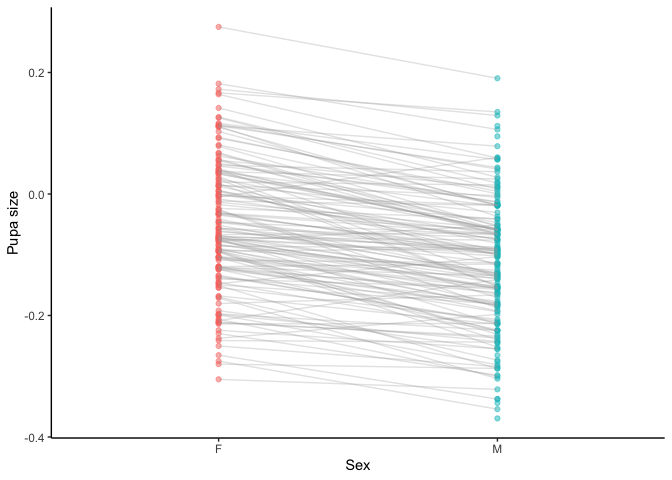
\includegraphics{_PreliminaryAnalysis_files/figure-latex/unnamed-chunk-32-1.pdf}
SSD decreases at Day1 starvation but seems to reincrease at day2, let's
check if this is significant

I just want to compare the means of SSD.

\begin{Shaded}
\begin{Highlighting}[]
\CommentTok{#ANOVA on SSD per day}
\KeywordTok{head}\NormalTok{(SSD_all)}
\end{Highlighting}
\end{Shaded}

\begin{verbatim}
##   line        SSD day
## 1 L100 0.13857467  D0
## 2 L101 0.01938781  D0
## 3 L105 0.04979026  D0
## 4 L109 0.08337778  D0
## 5 L136 0.11563351  D0
## 6 L138 0.08666043  D0
\end{verbatim}

\begin{Shaded}
\begin{Highlighting}[]
\NormalTok{SSDtest<-}\KeywordTok{aov}\NormalTok{(}\DataTypeTok{data=}\NormalTok{SSD_all, SSD }\OperatorTok{~}\NormalTok{day)}
\KeywordTok{summary}\NormalTok{(SSDtest)}
\end{Highlighting}
\end{Shaded}

\begin{verbatim}
##              Df Sum Sq Mean Sq F value   Pr(>F)    
## day           2  0.067 0.03349      13 3.42e-06 ***
## Residuals   395  1.018 0.00258                     
## ---
## Signif. codes:  0 '***' 0.001 '**' 0.01 '*' 0.05 '.' 0.1 ' ' 1
\end{verbatim}

\begin{Shaded}
\begin{Highlighting}[]
\KeywordTok{plot}\NormalTok{(SSDtest)}
\end{Highlighting}
\end{Shaded}

\includegraphics{_PreliminaryAnalysis_files/figure-latex/unnamed-chunk-33-1.pdf}
\includegraphics{_PreliminaryAnalysis_files/figure-latex/unnamed-chunk-33-2.pdf}
\includegraphics{_PreliminaryAnalysis_files/figure-latex/unnamed-chunk-33-3.pdf}
\includegraphics{_PreliminaryAnalysis_files/figure-latex/unnamed-chunk-33-4.pdf}

\begin{Shaded}
\begin{Highlighting}[]
\KeywordTok{model.tables}\NormalTok{(SSDtest, }\DataTypeTok{type=}\StringTok{"means"}\NormalTok{, }\DataTypeTok{se =} \OtherTok{TRUE}\NormalTok{)}
\end{Highlighting}
\end{Shaded}

\begin{verbatim}
## Design is unbalanced - use se.contrast() for se's
\end{verbatim}

\begin{verbatim}
## Tables of means
## Grand mean
##            
## 0.07954706 
## 
##  day 
##            D0        D1       D2
##       0.09325   0.06536  0.07505
## rep 182.00000 157.00000 59.00000
\end{verbatim}

\begin{Shaded}
\begin{Highlighting}[]
\CommentTok{#Pairwise comparison}
\KeywordTok{TukeyHSD}\NormalTok{(SSDtest, }\DataTypeTok{which =} \StringTok{"day"}\NormalTok{)}
\end{Highlighting}
\end{Shaded}

\begin{verbatim}
##   Tukey multiple comparisons of means
##     95% family-wise confidence level
## 
## Fit: aov(formula = SSD ~ day, data = SSD_all)
## 
## $day
##               diff          lwr           upr     p adj
## D1-D0 -0.027891722 -0.040899261 -0.0148841833 0.0000021
## D2-D0 -0.018196675 -0.036087387 -0.0003059631 0.0451745
## D2-D1  0.009695047 -0.008541048  0.0279311421 0.4240973
\end{verbatim}

SSD0 and SSD1 are significantly different, with SSD0 \textgreater{} SSD1
SSD0 and SSD2 are significantly different (p=0.0451745), SSD0
\textgreater{} SSD2 SSD1 and SSD2 are not significantly different

Starvation decreases SSD but it does not change at different levels of
starvation. high p value of SSD0 vs SSD2 due to low number of lines?
Should I fit lmer with day0 and day2 raw data subset instead?

\hypertarget{question-2.3-does-ssd-in-starved-conditions-vary-and-does-it-covary-with-ssd0}{%
\subsection{Question 2.3: Does SSD in starved conditions vary, and does
it covary with
SSD0?}\label{question-2.3-does-ssd-in-starved-conditions-vary-and-does-it-covary-with-ssd0}}

First, we want to see if there is genetic variation in SSD1 and SSD2
\#\#\# SSD1

\begin{Shaded}
\begin{Highlighting}[]
\CommentTok{#Comparing two model fit for SSD1 to see if there is genetic variation}

\NormalTok{model2<-}\KeywordTok{lmer}\NormalTok{(pupa}\OperatorTok{~}\NormalTok{sex}\OperatorTok{+}\NormalTok{(}\DecValTok{1}\OperatorTok{|}\NormalTok{line)}\OperatorTok{+}\NormalTok{(}\DecValTok{1}\OperatorTok{|}\NormalTok{block), }\DataTypeTok{data=}\NormalTok{df1)  }\CommentTok{#model to test for SSD presence as we did above}
\NormalTok{model1<-}\KeywordTok{lmer}\NormalTok{(pupa}\OperatorTok{~}\NormalTok{sex}\OperatorTok{+}\NormalTok{(sex}\OperatorTok{|}\NormalTok{line)}\OperatorTok{+}\NormalTok{(}\DecValTok{1}\OperatorTok{|}\NormalTok{block), }\DataTypeTok{data=}\NormalTok{df1) }
\KeywordTok{anova}\NormalTok{(model1)}
\end{Highlighting}
\end{Shaded}

\begin{verbatim}
## Type III Analysis of Variance Table with Satterthwaite's method
##     Sum Sq Mean Sq NumDF  DenDF F value    Pr(>F)    
## sex 4.1858  4.1858     1 166.44  242.44 < 2.2e-16 ***
## ---
## Signif. codes:  0 '***' 0.001 '**' 0.01 '*' 0.05 '.' 0.1 ' ' 1
\end{verbatim}

\begin{Shaded}
\begin{Highlighting}[]
\KeywordTok{anova}\NormalTok{(model1,model2)}
\end{Highlighting}
\end{Shaded}

\begin{verbatim}
## refitting model(s) with ML (instead of REML)
\end{verbatim}

\begin{verbatim}
## Data: df1
## Models:
## model2: pupa ~ sex + (1 | line) + (1 | block)
## model1: pupa ~ sex + (sex | line) + (1 | block)
##        npar     AIC     BIC logLik deviance  Chisq Df Pr(>Chisq)    
## model2    5 -7184.1 -7150.2 3597.0  -7194.1                         
## model1    7 -7198.5 -7151.2 3606.3  -7212.5 18.442  2  9.893e-05 ***
## ---
## Signif. codes:  0 '***' 0.001 '**' 0.01 '*' 0.05 '.' 0.1 ' ' 1
\end{verbatim}

Model 1 is better, as AIC and BIC is smaller and log likelihood is
higher. The difference of fit between these two models is significant.

\hypertarget{do-a-lrt-1}{%
\subsubsection{Do a LRT}\label{do-a-lrt-1}}

How many parameters for each models

\begin{Shaded}
\begin{Highlighting}[]
\NormalTok{(}\KeywordTok{AIC}\NormalTok{(model1) }\OperatorTok{-}\StringTok{ }\KeywordTok{REMLcrit}\NormalTok{(model1))}\OperatorTok{/}\DecValTok{2} \CommentTok{# # of parameters the model "thinks" are being estimated}
\end{Highlighting}
\end{Shaded}

\begin{verbatim}
## [1] 7
\end{verbatim}

\begin{Shaded}
\begin{Highlighting}[]
\NormalTok{(}\KeywordTok{AIC}\NormalTok{(model2) }\OperatorTok{-}\StringTok{ }\KeywordTok{REMLcrit}\NormalTok{(model2))}\OperatorTok{/}\DecValTok{2} \CommentTok{# # of parameters the model "thinks" are being estimated}
\end{Highlighting}
\end{Shaded}

\begin{verbatim}
## [1] 5
\end{verbatim}

So lme4/lmer is treating model 1 as having two more parameters than
model2.

\begin{Shaded}
\begin{Highlighting}[]
\NormalTok{LR.model <-}\StringTok{  }\OperatorTok{-}\KeywordTok{as.numeric}\NormalTok{(}\KeywordTok{REMLcrit}\NormalTok{(model1) }\OperatorTok{-}\StringTok{ }\KeywordTok{REMLcrit}\NormalTok{(model2))}
\NormalTok{LR.model}
\end{Highlighting}
\end{Shaded}

\begin{verbatim}
## [1] 18.79382
\end{verbatim}

\begin{Shaded}
\begin{Highlighting}[]
\KeywordTok{nlevels}\NormalTok{(df1}\OperatorTok{$}\NormalTok{line)}
\end{Highlighting}
\end{Shaded}

\begin{verbatim}
## [1] 0
\end{verbatim}

\begin{Shaded}
\begin{Highlighting}[]
\KeywordTok{pchisq}\NormalTok{(}\DataTypeTok{q =}\NormalTok{ LR.model, }\DataTypeTok{df=}\DecValTok{2}\NormalTok{, }\DataTypeTok{lower=}\NormalTok{F)}
\end{Highlighting}
\end{Shaded}

\begin{verbatim}
## [1] 8.297996e-05
\end{verbatim}

\begin{Shaded}
\begin{Highlighting}[]
\KeywordTok{pchisq}\NormalTok{(}\DataTypeTok{q =}\NormalTok{ LR.model, }\DataTypeTok{df=}\KeywordTok{nlevels}\NormalTok{(df1}\OperatorTok{$}\NormalTok{line), }\DataTypeTok{lower=}\NormalTok{F)}
\end{Highlighting}
\end{Shaded}

\begin{verbatim}
## [1] 0
\end{verbatim}

\hypertarget{parametric-boostrap-1}{%
\subsubsection{Parametric boostrap}\label{parametric-boostrap-1}}

Finally, we can conduct a parametric bootstrap to compare the two
models.

\hypertarget{finally-using-bayesian-analysis-1}{%
\subsubsection{Finally using Bayesian
Analysis}\label{finally-using-bayesian-analysis-1}}

\begin{Shaded}
\begin{Highlighting}[]
\CommentTok{#prior.2 <-list(R=list(V=0.01, nu=0.002), }
\CommentTok{#               G=list(G1=list(V=0.01*diag(1), nu=0.002),}
 \CommentTok{#                     G2=list(V=0.01*diag(2), nu=0.002)))}

\CommentTok{#model1M.MCMC <- MCMCglmm(pupa ~ 1 + sex, }
\CommentTok{#  random=~block + us(1 + sex):line,}
 \CommentTok{# prior = prior.2, burnin = 5000, nitt = 20000, thin = 10,}
\CommentTok{#  verbose = F, pr = T,}
 \CommentTok{# data=df1)}
\CommentTok{#summary(model1M.MCMC)}
\end{Highlighting}
\end{Shaded}

\hypertarget{post-model-1-fitting-check-1}{%
\subsubsection{Post model 1 fitting
check}\label{post-model-1-fitting-check-1}}

\hypertarget{residual-distribution-1}{%
\paragraph{Residual distribution}\label{residual-distribution-1}}

\begin{Shaded}
\begin{Highlighting}[]
\NormalTok{res_model1=}\KeywordTok{residuals}\NormalTok{(model1)}
\end{Highlighting}
\end{Shaded}

\hypertarget{model-1-residual-distribution-1}{%
\paragraph{Model 1 residual
distribution}\label{model-1-residual-distribution-1}}

\begin{Shaded}
\begin{Highlighting}[]
\KeywordTok{plot}\NormalTok{(model1)}
\end{Highlighting}
\end{Shaded}

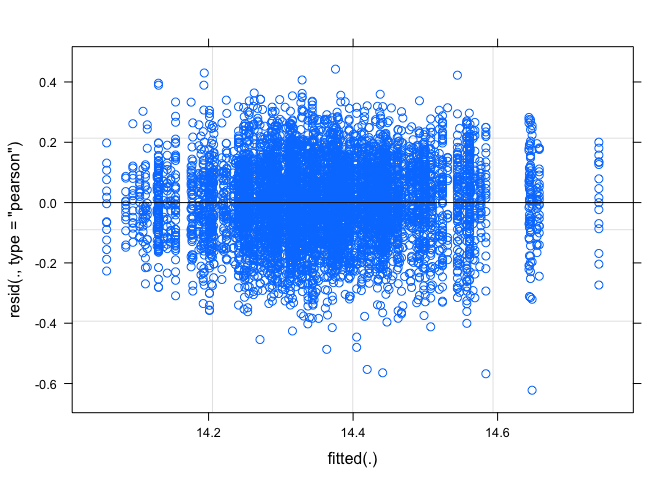
\includegraphics{_PreliminaryAnalysis_files/figure-latex/unnamed-chunk-40-1.pdf}

\hypertarget{qq-plot-1}{%
\paragraph{QQ plot}\label{qq-plot-1}}

\begin{Shaded}
\begin{Highlighting}[]
\KeywordTok{require}\NormalTok{(ggpubr)}
\KeywordTok{ggqqplot}\NormalTok{(res_model1)}
\end{Highlighting}
\end{Shaded}

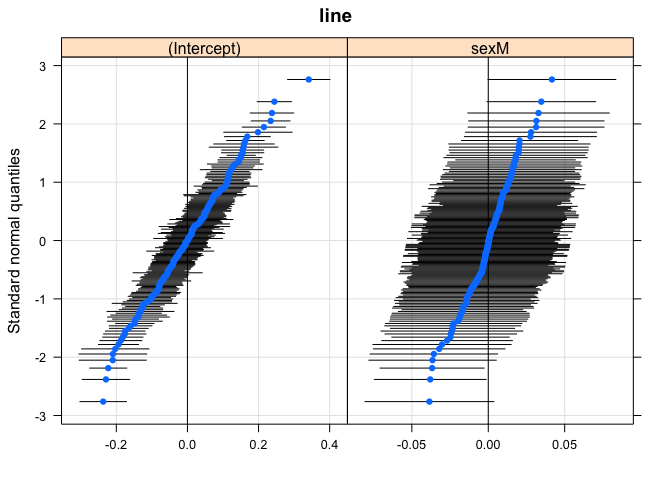
\includegraphics{_PreliminaryAnalysis_files/figure-latex/unnamed-chunk-41-1.pdf}

\hypertarget{random-effect-plot-1}{%
\paragraph{Random effect plot}\label{random-effect-plot-1}}

\begin{Shaded}
\begin{Highlighting}[]
\KeywordTok{qqmath}\NormalTok{(}\KeywordTok{ranef}\NormalTok{(model1))}
\end{Highlighting}
\end{Shaded}

\begin{verbatim}
## $line
\end{verbatim}

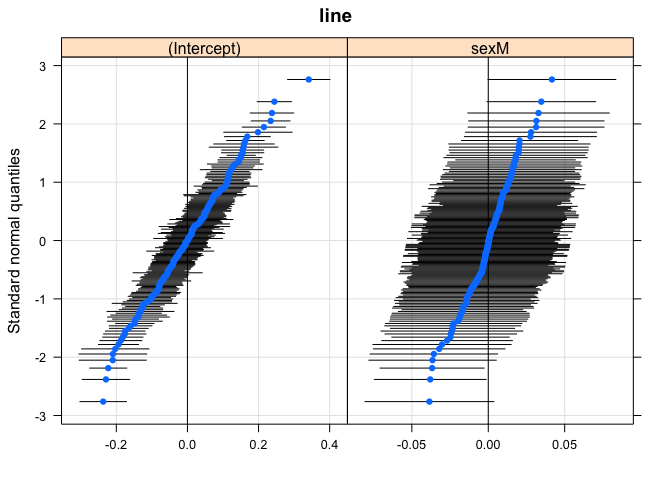
\includegraphics{_PreliminaryAnalysis_files/figure-latex/unnamed-chunk-42-1.pdf}

\begin{verbatim}
## 
## $block
\end{verbatim}

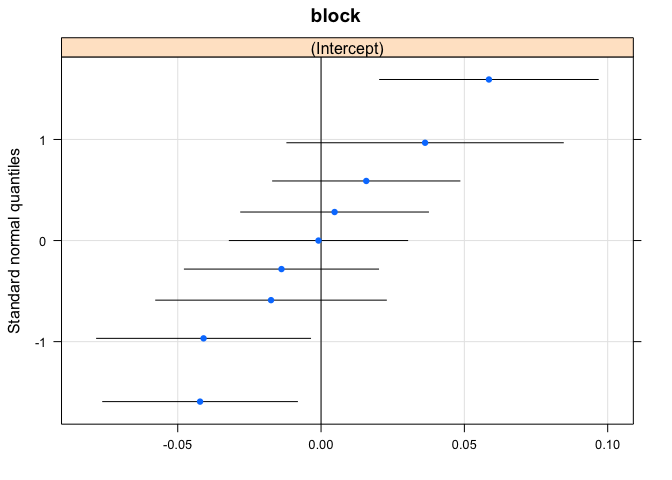
\includegraphics{_PreliminaryAnalysis_files/figure-latex/unnamed-chunk-42-2.pdf}

\hypertarget{ssd2}{%
\subsubsection{SSD2}\label{ssd2}}

\begin{Shaded}
\begin{Highlighting}[]
\CommentTok{#Comparing two model fit for SSD2 to see if there is genetic variation}

\NormalTok{model2<-}\KeywordTok{lmer}\NormalTok{(pupa}\OperatorTok{~}\NormalTok{sex}\OperatorTok{+}\NormalTok{(}\DecValTok{1}\OperatorTok{|}\NormalTok{line)}\OperatorTok{+}\NormalTok{(}\DecValTok{1}\OperatorTok{|}\NormalTok{block), }\DataTypeTok{data=}\NormalTok{df2)  }\CommentTok{#model to test for SSD presence as we did above}
\NormalTok{model1<-}\KeywordTok{lmer}\NormalTok{(pupa}\OperatorTok{~}\NormalTok{sex}\OperatorTok{+}\NormalTok{(sex}\OperatorTok{|}\NormalTok{line)}\OperatorTok{+}\NormalTok{(}\DecValTok{1}\OperatorTok{|}\NormalTok{block), }\DataTypeTok{data=}\NormalTok{df2) }
\end{Highlighting}
\end{Shaded}

\begin{verbatim}
## boundary (singular) fit: see ?isSingular
\end{verbatim}

\begin{Shaded}
\begin{Highlighting}[]
\KeywordTok{anova}\NormalTok{(model1)}
\end{Highlighting}
\end{Shaded}

\begin{verbatim}
## Type III Analysis of Variance Table with Satterthwaite's method
##     Sum Sq Mean Sq NumDF  DenDF F value    Pr(>F)    
## sex  2.998   2.998     1 227.51  220.25 < 2.2e-16 ***
## ---
## Signif. codes:  0 '***' 0.001 '**' 0.01 '*' 0.05 '.' 0.1 ' ' 1
\end{verbatim}

\begin{Shaded}
\begin{Highlighting}[]
\KeywordTok{anova}\NormalTok{(model1,model2)}
\end{Highlighting}
\end{Shaded}

\begin{verbatim}
## refitting model(s) with ML (instead of REML)
\end{verbatim}

\begin{verbatim}
## Data: df2
## Models:
## model2: pupa ~ sex + (1 | line) + (1 | block)
## model1: pupa ~ sex + (sex | line) + (1 | block)
##        npar     AIC     BIC logLik deviance  Chisq Df Pr(>Chisq)  
## model2    5 -3605.6 -3576.1 1807.8  -3615.6                       
## model1    7 -3608.9 -3567.7 1811.5  -3622.9 7.3459  2     0.0254 *
## ---
## Signif. codes:  0 '***' 0.001 '**' 0.01 '*' 0.05 '.' 0.1 ' ' 1
\end{verbatim}

Model 1 is better, as AIC and BIC is smaller and log likelihood is
higher. The difference of fit between these two models is significant.

\hypertarget{do-a-lrt-2}{%
\subsubsection{Do a LRT}\label{do-a-lrt-2}}

How many parameters for each models

\begin{Shaded}
\begin{Highlighting}[]
\NormalTok{(}\KeywordTok{AIC}\NormalTok{(model1) }\OperatorTok{-}\StringTok{ }\KeywordTok{REMLcrit}\NormalTok{(model1))}\OperatorTok{/}\DecValTok{2} \CommentTok{# # of parameters the model "thinks" are being estimated}
\end{Highlighting}
\end{Shaded}

\begin{verbatim}
## [1] 7
\end{verbatim}

\begin{Shaded}
\begin{Highlighting}[]
\NormalTok{(}\KeywordTok{AIC}\NormalTok{(model2) }\OperatorTok{-}\StringTok{ }\KeywordTok{REMLcrit}\NormalTok{(model2))}\OperatorTok{/}\DecValTok{2} \CommentTok{# # of parameters the model "thinks" are being estimated}
\end{Highlighting}
\end{Shaded}

\begin{verbatim}
## [1] 5
\end{verbatim}

So lme4/lmer is treating model 1 as having two more parameters than
model2.

\begin{Shaded}
\begin{Highlighting}[]
\NormalTok{LR.model <-}\StringTok{  }\OperatorTok{-}\KeywordTok{as.numeric}\NormalTok{(}\KeywordTok{REMLcrit}\NormalTok{(model1) }\OperatorTok{-}\StringTok{ }\KeywordTok{REMLcrit}\NormalTok{(model2))}
\NormalTok{LR.model}
\end{Highlighting}
\end{Shaded}

\begin{verbatim}
## [1] 7.454988
\end{verbatim}

\begin{Shaded}
\begin{Highlighting}[]
\KeywordTok{nlevels}\NormalTok{(df2}\OperatorTok{$}\NormalTok{line)}
\end{Highlighting}
\end{Shaded}

\begin{verbatim}
## [1] 0
\end{verbatim}

\begin{Shaded}
\begin{Highlighting}[]
\KeywordTok{pchisq}\NormalTok{(}\DataTypeTok{q =}\NormalTok{ LR.model, }\DataTypeTok{df=}\DecValTok{2}\NormalTok{, }\DataTypeTok{lower=}\NormalTok{F)}
\end{Highlighting}
\end{Shaded}

\begin{verbatim}
## [1] 0.02405304
\end{verbatim}

\begin{Shaded}
\begin{Highlighting}[]
\KeywordTok{pchisq}\NormalTok{(}\DataTypeTok{q =}\NormalTok{ LR.model, }\DataTypeTok{df=}\KeywordTok{nlevels}\NormalTok{(df2}\OperatorTok{$}\NormalTok{line), }\DataTypeTok{lower=}\NormalTok{F)}
\end{Highlighting}
\end{Shaded}

\begin{verbatim}
## [1] 0
\end{verbatim}

\hypertarget{parametric-boostrap-2}{%
\subsubsection{Parametric boostrap}\label{parametric-boostrap-2}}

Finally, we can conduct a parametric bootstrap to compare the two
models.

\hypertarget{finally-using-bayesian-analysis-2}{%
\subsubsection{Finally using Bayesian
Analysis}\label{finally-using-bayesian-analysis-2}}

\begin{Shaded}
\begin{Highlighting}[]
\CommentTok{#prior.2 <-list(R=list(V=0.01, nu=0.002), }
 \CommentTok{#              G=list(G1=list(V=0.01*diag(1), nu=0.002),}
  \CommentTok{#                    G2=list(V=0.01*diag(2), nu=0.002)))}

\CommentTok{#model1M.MCMC <- MCMCglmm(pupa ~ 1 + sex, }
 \CommentTok{# random=~block + us(1 + sex):line,}
  \CommentTok{#prior = prior.2, burnin = 5000, nitt = 20000, thin = 10,}
\CommentTok{# verbose = F, pr = T,}
 \CommentTok{# data=df2)}
\CommentTok{#summary(model1M.MCMC)}
\end{Highlighting}
\end{Shaded}

\hypertarget{post-model-1-fitting-check-2}{%
\subsubsection{Post model 1 fitting
check}\label{post-model-1-fitting-check-2}}

\hypertarget{residual-distribution-2}{%
\paragraph{Residual distribution}\label{residual-distribution-2}}

\begin{Shaded}
\begin{Highlighting}[]
\NormalTok{res_model1=}\KeywordTok{residuals}\NormalTok{(model1)}
\end{Highlighting}
\end{Shaded}

\hypertarget{model-1-residual-distribution-2}{%
\paragraph{Model 1 residual
distribution}\label{model-1-residual-distribution-2}}

\begin{Shaded}
\begin{Highlighting}[]
\KeywordTok{plot}\NormalTok{(model1)}
\end{Highlighting}
\end{Shaded}

\includegraphics{_PreliminaryAnalysis_files/figure-latex/unnamed-chunk-49-1.pdf}

\hypertarget{qq-plot-2}{%
\paragraph{QQ plot}\label{qq-plot-2}}

\begin{Shaded}
\begin{Highlighting}[]
\KeywordTok{require}\NormalTok{(ggpubr)}
\KeywordTok{ggqqplot}\NormalTok{(res_model1)}
\end{Highlighting}
\end{Shaded}

\includegraphics{_PreliminaryAnalysis_files/figure-latex/unnamed-chunk-50-1.pdf}

\hypertarget{random-effect-plot-2}{%
\paragraph{Random effect plot}\label{random-effect-plot-2}}

\begin{Shaded}
\begin{Highlighting}[]
\KeywordTok{qqmath}\NormalTok{(}\KeywordTok{ranef}\NormalTok{(model1))}
\end{Highlighting}
\end{Shaded}

\begin{verbatim}
## $line
\end{verbatim}

\includegraphics{_PreliminaryAnalysis_files/figure-latex/unnamed-chunk-51-1.pdf}

\begin{verbatim}
## 
## $block
\end{verbatim}

\includegraphics{_PreliminaryAnalysis_files/figure-latex/unnamed-chunk-51-2.pdf}
We have two plots, one for line and one for block

SSD1 and SSD2 vary also significantly.

Does that variation correlate with SSD0?

If SSD0 covaries with SSD1/SSD2, that means we should not see a
difference in plasticity. We first can visualize how SSD changes across
lineages.

\begin{Shaded}
\begin{Highlighting}[]
\KeywordTok{ggplot}\NormalTok{(SSD_all, }\KeywordTok{aes}\NormalTok{(}\DataTypeTok{x=}\KeywordTok{reorder}\NormalTok{(line,SSD), }\DataTypeTok{y=}\NormalTok{SSD)) }\OperatorTok{+}
\StringTok{  }\KeywordTok{geom_col}\NormalTok{(}\KeywordTok{aes}\NormalTok{(}\DataTypeTok{fill =}\NormalTok{ day)) }\OperatorTok{+}
\StringTok{  }\KeywordTok{facet_wrap}\NormalTok{(}\OperatorTok{~}\StringTok{ }\NormalTok{day) }\OperatorTok{+}
\StringTok{  }\KeywordTok{coord_flip}\NormalTok{()}
\end{Highlighting}
\end{Shaded}

\includegraphics{_PreliminaryAnalysis_files/figure-latex/unnamed-chunk-52-1.pdf}
Correlation between SSDs. Hypothesis, if SSD changes with environment,
which is what we expect, we will not see a correlation between SSD0 and
SSD1 and/or SSD2

\begin{Shaded}
\begin{Highlighting}[]
\CommentTok{#correlation SSD0, SSD1, SSD2}
\NormalTok{SSD_all_col<-}\KeywordTok{spread}\NormalTok{(SSD_all,day ,SSD)}

\KeywordTok{head}\NormalTok{(SSD_all_col) }\CommentTok{#D0 is SSD0, D1 is SSD1 and D2 is SSD2}
\end{Highlighting}
\end{Shaded}

\begin{verbatim}
##   line         D0         D1 D2
## 1 L100 0.13857467 0.02501154 NA
## 2 L101 0.01938781 0.06558689 NA
## 3 L105 0.04979026 0.16674254 NA
## 4 L109 0.08337778 0.10647941 NA
## 5 L129         NA 0.08614931 NA
## 6 L136 0.11563351 0.04728358 NA
\end{verbatim}

\begin{Shaded}
\begin{Highlighting}[]
\KeywordTok{corr.test}\NormalTok{(SSD_all_col[}\DecValTok{2}\OperatorTok{:}\DecValTok{4}\NormalTok{],}
          \DataTypeTok{use    =} \StringTok{"pairwise"}\NormalTok{,}
          \DataTypeTok{method =} \StringTok{"pearson"}\NormalTok{,}
          \DataTypeTok{adjust =} \StringTok{"none"}\NormalTok{)}
\end{Highlighting}
\end{Shaded}

\begin{verbatim}
## Call:corr.test(x = SSD_all_col[2:4], use = "pairwise", method = "pearson", 
##     adjust = "none")
## Correlation matrix 
##      D0    D1    D2
## D0 1.00  0.19  0.34
## D1 0.19  1.00 -0.12
## D2 0.34 -0.12  1.00
## Sample Size 
##     D0  D1 D2
## D0 182 146 55
## D1 146 157 51
## D2  55  51 59
## Probability values (Entries above the diagonal are adjusted for multiple tests.) 
##      D0   D1   D2
## D0 0.00 0.02 0.01
## D1 0.02 0.00 0.40
## D2 0.01 0.40 0.00
## 
##  To see confidence intervals of the correlations, print with the short=FALSE option
\end{verbatim}

\begin{Shaded}
\begin{Highlighting}[]
\KeywordTok{chart.Correlation}\NormalTok{(SSD_all_col[}\DecValTok{2}\OperatorTok{:}\DecValTok{4}\NormalTok{],}
                   \DataTypeTok{method=}\StringTok{"pearson"}\NormalTok{,}
                   \DataTypeTok{histogram=}\OtherTok{TRUE}\NormalTok{,}
                   \DataTypeTok{pch=}\DecValTok{16}\NormalTok{)}
\end{Highlighting}
\end{Shaded}

\includegraphics{_PreliminaryAnalysis_files/figure-latex/unnamed-chunk-53-1.pdf}
There is a weak correlation between SSD0 and SSD2, still higher than
SSD1 and SSD0

Since there is just a weak correlation between SSD0 and SSD2, I want to
know if SSD1 and SSD2 varies because of female size variation as it was
found in SSD0.

Correlation SSD2 and female and male size

\begin{Shaded}
\begin{Highlighting}[]
\CommentTok{#SSD2 and female and male size dataset}
\NormalTok{df2_mean}
\end{Highlighting}
\end{Shaded}

\begin{verbatim}
##    line        pupaF2       pupaM2          SSD2
## 1  L153  0.2083490996  0.086998187  0.1213509129
## 2  L158  0.0198706211 -0.072010303  0.0918809238
## 3  L229  0.0252440717 -0.171367258  0.1966113298
## 4  L256 -0.0510827809 -0.174299175  0.1232163941
## 5   L26 -0.0020925854 -0.104164760  0.1020721748
## 6   L28  0.0920290502 -0.003598201  0.0956272516
## 7  L313 -0.1179784463 -0.096055488 -0.0219229586
## 8  L315 -0.1372958724 -0.227830626  0.0905347537
## 9  L319 -0.1905172024 -0.263133001  0.0726157989
## 10 L320 -0.0151649423 -0.092589150  0.0774242074
## 11 L338 -0.2255686647 -0.212390102 -0.0131785622
## 12 L354 -0.0808734568 -0.178212569  0.0973391121
## 13 L362 -0.0422510651 -0.147820521  0.1055694556
## 14 L367 -0.2825281894 -0.320091371  0.0375631812
## 15 L371 -0.2004012237 -0.253068519  0.0526672950
## 16  L38 -0.0307460122 -0.116562063  0.0858160511
## 17 L383 -0.0190385109 -0.178242643  0.1592041318
## 18 L390 -0.0147332607 -0.076423444  0.0616901830
## 19 L391 -0.2205041647 -0.191912421 -0.0285917437
## 20 L392 -0.1719153572 -0.223307799  0.0513924419
## 21 L405 -0.2012851854 -0.271726019  0.0704408335
## 22 L406 -0.0657860658 -0.136983977  0.0711979112
## 23 L409 -0.0172878930 -0.096135443  0.0788475499
## 24 L437 -0.0977846693 -0.184148632  0.0863639631
## 25 L440 -0.1554390872 -0.241890393  0.0864513057
## 26 L505  0.0429097802 -0.046799809  0.0897095890
## 27 L509  0.2485134551  0.143144992  0.1053684634
## 28 L513 -0.2903689004 -0.300403284  0.0100343836
## 29 L530 -0.2497311785 -0.258857879  0.0091267004
## 30 L566 -0.0735318015 -0.114252463  0.0407206611
## 31 L584 -0.0309484196 -0.143715889  0.1127674696
## 32 L596 -0.2030872174 -0.285939676  0.0828524586
## 33 L627 -0.0636625560 -0.101912163  0.0382496069
## 34 L630 -0.0005452741 -0.083705399  0.0831601245
## 35 L634  0.0065391132 -0.104956480  0.1114955928
## 36 L646 -0.0121977293 -0.096034716  0.0838369868
## 37 L703 -0.2122686207 -0.280064183  0.0677955625
## 38 L705 -0.1351255876 -0.182334959  0.0472093713
## 39 L727 -0.0033413430 -0.115717830  0.1123764871
## 40 L730  0.1447091845  0.070755243  0.0739539418
## 41 L732 -0.0052659063 -0.164331749  0.1590658429
## 42 L786 -0.2229516599 -0.381456201  0.1585045410
## 43 L802 -0.0854357841 -0.159692046  0.0742562620
## 44 L810  0.0376951127 -0.045968804  0.0836639167
## 45 L818 -0.2296882300 -0.242228125  0.0125398951
## 46 L821 -0.1137744961 -0.234764347  0.1209898510
## 47 L822 -0.0169807339 -0.105745285  0.0887645512
## 48 L837 -0.1138931961 -0.140305873  0.0264126771
## 49  L85 -0.0835950963 -0.197718003  0.1141229063
## 50 L852 -0.2130209089 -0.266100892  0.0530799829
## 51 L857 -0.1652272431 -0.221544321  0.0563170783
## 52 L859 -0.1076108039 -0.232294681  0.1246838774
## 53 L892 -0.1948029739 -0.171113704 -0.0236892699
## 54 L894  0.1200987491  0.040896105  0.0792026444
## 55 L897 -0.2552249009 -0.255385553  0.0001606525
## 56 L907  0.0151010709 -0.010220978  0.0253220485
## 57  L91 -0.1265304597 -0.246215481  0.1196850217
## 58 L911 -0.3148649245 -0.330165402  0.0153004776
## 59 L913 -0.2404059087 -0.359154738  0.1187488294
\end{verbatim}

\begin{Shaded}
\begin{Highlighting}[]
\KeywordTok{corr.test}\NormalTok{(df2_mean[}\DecValTok{2}\OperatorTok{:}\DecValTok{4}\NormalTok{],}
          \DataTypeTok{use    =} \StringTok{"pairwise"}\NormalTok{,}
          \DataTypeTok{method =} \StringTok{"pearson"}\NormalTok{,}
          \DataTypeTok{adjust =} \StringTok{"none"}\NormalTok{)}
\end{Highlighting}
\end{Shaded}

\begin{verbatim}
## Call:corr.test(x = df2_mean[2:4], use = "pairwise", method = "pearson", 
##     adjust = "none")
## Correlation matrix 
##        pupaF2 pupaM2 SSD2
## pupaF2   1.00   0.92 0.48
## pupaM2   0.92   1.00 0.11
## SSD2     0.48   0.11 1.00
## Sample Size 
## [1] 59
## Probability values (Entries above the diagonal are adjusted for multiple tests.) 
##        pupaF2 pupaM2 SSD2
## pupaF2      0    0.0  0.0
## pupaM2      0    0.0  0.4
## SSD2        0    0.4  0.0
## 
##  To see confidence intervals of the correlations, print with the short=FALSE option
\end{verbatim}

\begin{Shaded}
\begin{Highlighting}[]
\CommentTok{#correlation plot}
\KeywordTok{chart.Correlation}\NormalTok{(df2_mean[}\DecValTok{2}\OperatorTok{:}\DecValTok{4}\NormalTok{],}
                   \DataTypeTok{method=}\StringTok{"pearson"}\NormalTok{,}
                   \DataTypeTok{histogram=}\OtherTok{TRUE}\NormalTok{,}
                   \DataTypeTok{pch=}\DecValTok{16}\NormalTok{)}
\end{Highlighting}
\end{Shaded}

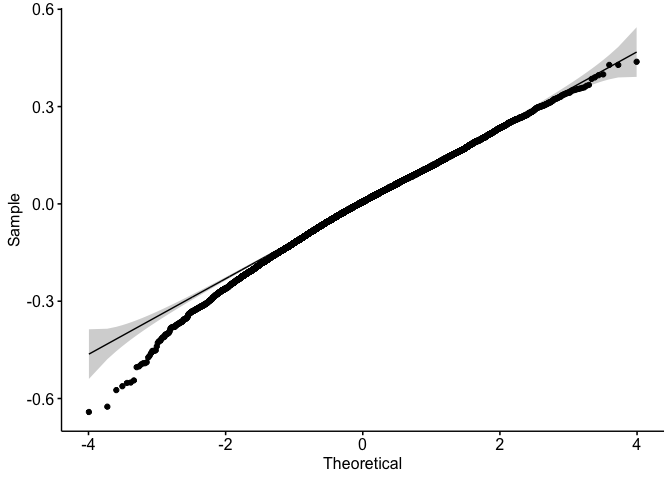
\includegraphics{_PreliminaryAnalysis_files/figure-latex/unnamed-chunk-55-1.pdf}

SSD2 covaries with female size in 2 days starvation.

Will still check SSD1, even though it does not correlate with SSD0, we
can see if SSD1 variation covaries with either female or male variation

\begin{Shaded}
\begin{Highlighting}[]
\CommentTok{#SSD2 and female and male size dataset}
\NormalTok{df1_mean}
\end{Highlighting}
\end{Shaded}

\begin{verbatim}
##     line        pupaF1        pupaM1          SSD1
## 1   L100  0.0851532538  0.0601417184  2.501154e-02
## 2   L101 -0.0352033147 -0.1007902097  6.558689e-02
## 3   L105 -0.0847950896 -0.2515376332  1.667425e-01
## 4   L109 -0.1524421631 -0.2589215723  1.064794e-01
## 5   L129  0.0498926174 -0.0362566925  8.614931e-02
## 6   L136 -0.0958005906 -0.1430841729  4.728358e-02
## 7   L138 -0.0094674828 -0.0431888766  3.372139e-02
## 8   L142  0.1912391953  0.0679039676  1.233352e-01
## 9   L149  0.0824609832 -0.0435773959  1.260384e-01
## 10  L153  0.1882480349  0.0823996337  1.058484e-01
## 11  L176 -0.1741861063 -0.2186190720  4.443297e-02
## 12  L177 -0.0995002522 -0.1514573520  5.195710e-02
## 13  L181  0.0550627316 -0.1353124598  1.903752e-01
## 14  L189 -0.2046822969 -0.2060623524  1.380056e-03
## 15  L208 -0.1352973339 -0.2094715748  7.417424e-02
## 16   L21  0.1028552450  0.0066296633  9.622558e-02
## 17  L217 -0.0176038950 -0.1728636819  1.552598e-01
## 18  L227  0.0273039358 -0.0802281974  1.075321e-01
## 19  L228 -0.2507560950 -0.3169567326  6.620064e-02
## 20  L235 -0.2890087692 -0.3244309568  3.542219e-02
## 21  L237 -0.0559139374 -0.1982819629  1.423680e-01
## 22  L239 -0.0589207423 -0.1214962535  6.257551e-02
## 23  L256 -0.1306209909 -0.1203311005 -1.028989e-02
## 24   L26 -0.0770550771 -0.1362855302  5.923045e-02
## 25   L28  0.1986955678  0.1082339500  9.046162e-02
## 26  L280 -0.0257489620 -0.0996427476  7.389379e-02
## 27  L301 -0.0815394744 -0.1481846753  6.664520e-02
## 28  L303 -0.0533939036 -0.1278199677  7.442606e-02
## 29  L306  0.1217251138 -0.0269067432  1.486319e-01
## 30  L307 -0.0363624890 -0.0797948471  4.343236e-02
## 31  L309  0.1097901170  0.0566497205  5.314040e-02
## 32   L31  0.0346798423 -0.0105697357  4.524958e-02
## 33  L310 -0.1759958564 -0.2413176519  6.532180e-02
## 34  L313 -0.0071908668 -0.0368514543  2.966059e-02
## 35  L315  0.1312932781  0.0131678887  1.181254e-01
## 36  L317 -0.1351926442 -0.2489163673  1.137237e-01
## 37  L318 -0.0553737395 -0.1206807887  6.530705e-02
## 38  L319  0.0632398542 -0.0731527138  1.363926e-01
## 39   L32 -0.0473207791 -0.0934384653  4.611769e-02
## 40  L320 -0.0661455814 -0.1538200542  8.767447e-02
## 41  L324 -0.0959686164 -0.1157699693  1.980135e-02
## 42  L335 -0.1217581769 -0.1751294395  5.337126e-02
## 43  L338  0.0645450800 -0.0401475462  1.046926e-01
## 44  L340  0.0098509727  0.0208099591 -1.095899e-02
## 45  L350 -0.1421705189 -0.2299365315  8.776601e-02
## 46  L352 -0.2194042401 -0.2785213696  5.911713e-02
## 47  L354  0.1427723027  0.0369516658  1.058206e-01
## 48  L357 -0.1658311700 -0.1516326829 -1.419849e-02
## 49  L358 -0.1944352353 -0.2263989263  3.196369e-02
## 50  L359 -0.0296349961 -0.0211401559 -8.494840e-03
## 51  L360 -0.1251716548 -0.1265225715  1.350917e-03
## 52  L361 -0.0665855748 -0.0824244482  1.583887e-02
## 53  L362  0.1181650259 -0.0088624452  1.270275e-01
## 54  L365 -0.1262828634 -0.0904138463 -3.586902e-02
## 55  L367  0.0568802590 -0.0516140851  1.084943e-01
## 56  L371  0.0648859406 -0.1043776360  1.692636e-01
## 57  L373 -0.1611182266 -0.2452110473  8.409282e-02
## 58  L374  0.0290801502 -0.0609862173  9.006637e-02
## 59  L375 -0.1198272232 -0.1622562492  4.242903e-02
## 60  L379 -0.0701910858 -0.1542748022  8.408372e-02
## 61  L380  0.0286439653 -0.1368745675  1.655185e-01
## 62  L381  0.0721010793 -0.0752923001  1.473934e-01
## 63  L383  0.0012504628 -0.0012832047  2.533668e-03
## 64  L386  0.0007251280 -0.0551583444  5.588347e-02
## 65  L391  0.0414533853  0.0180386518  2.341473e-02
## 66  L392 -0.0527858797 -0.0233633394 -2.942254e-02
## 67  L395  0.0193872273  0.0244792428 -5.092016e-03
## 68  L397  0.1620890170  0.0353909089  1.266981e-01
## 69  L399 -0.0267094216 -0.1176703376  9.096092e-02
## 70  L405 -0.0688754198 -0.1059597491  3.708433e-02
## 71  L406  0.0082647715  0.0012416842  7.023087e-03
## 72   L42 -0.0393863809 -0.1501695621  1.107832e-01
## 73  L426 -0.1576390877 -0.2653843303  1.077452e-01
## 74  L427 -0.0027782274 -0.0481275156  4.534929e-02
## 75  L437 -0.1354031952 -0.1692003744  3.379718e-02
## 76  L440 -0.0318302952 -0.1045963742  7.276608e-02
## 77  L441 -0.0717971212 -0.1392467551  6.744963e-02
## 78  L461 -0.1308034201 -0.2106650955  7.986168e-02
## 79   L48  0.1904535545  0.1484298239  4.202373e-02
## 80  L491 -0.1242141126 -0.2017495714  7.753546e-02
## 81  L492 -0.1606280293 -0.2561454397  9.551741e-02
## 82  L502 -0.0489046761 -0.1360075709  8.710289e-02
## 83  L505 -0.0410824128 -0.0308193340 -1.026308e-02
## 84  L508  0.0176999682 -0.0727247119  9.042468e-02
## 85  L509  0.1834385767  0.1585592659  2.487931e-02
## 86  L513 -0.1760014084 -0.2010581300  2.505672e-02
## 87  L517 -0.1147505269 -0.2663424653  1.515919e-01
## 88  L530  0.0553797238 -0.0550014549  1.103812e-01
## 89  L535 -0.0319743497 -0.1705025420  1.385282e-01
## 90  L551  0.0988312345 -0.0375684555  1.363997e-01
## 91  L555  0.0307411797 -0.0574884864  8.822967e-02
## 92  L559 -0.0970450196 -0.1574232220  6.037820e-02
## 93  L584 -0.0586824853  0.0005649932 -5.924748e-02
## 94   L59 -0.1545108120 -0.2142769727  5.976616e-02
## 95  L595 -0.2596846418 -0.2622240597  2.539418e-03
## 96  L596 -0.0616550000 -0.1530820900  9.142709e-02
## 97  L627  0.0194556502 -0.0219055052  4.136116e-02
## 98  L634  0.0726465863  0.0512930229  2.135356e-02
## 99  L639 -0.2037562048 -0.2027810391 -9.751657e-04
## 100 L646  0.0823160402 -0.0354016691  1.177177e-01
## 101  L69 -0.0831740784 -0.2074156626  1.242416e-01
## 102 L703 -0.2190179360 -0.1705699992 -4.844794e-02
## 103 L705  0.1062921115 -0.0045373878  1.108295e-01
## 104 L707  0.0354973320 -0.1046154970  1.401128e-01
## 105 L714 -0.0540827359 -0.0733640931  1.928136e-02
## 106 L716 -0.0694542625 -0.0812645920  1.181033e-02
## 107 L721 -0.0984990664 -0.1777624587  7.926339e-02
## 108 L727 -0.0466060404 -0.0828274334  3.622139e-02
## 109  L73  0.0830990796  0.0145187632  6.858032e-02
## 110 L730  0.0059157279  0.0792157175 -7.329999e-02
## 111 L732  0.0051199960 -0.0670714545  7.219145e-02
## 112 L737  0.0731421536  0.0006543919  7.248776e-02
## 113 L748 -0.0549062290 -0.1244154701  6.950924e-02
## 114  L75 -0.1321925892 -0.1661190626  3.392647e-02
## 115 L757  0.0327562499  0.0013298605  3.142639e-02
## 116 L774 -0.0900913049 -0.1990423409  1.089510e-01
## 117 L776 -0.0315579656 -0.0834855246  5.192756e-02
## 118 L783  0.0001139527 -0.0398862067  4.000016e-02
## 119 L786 -0.0987282752 -0.1884320109  8.970374e-02
## 120 L787 -0.1004798267 -0.0962357964 -4.244030e-03
## 121 L790 -0.0584124918 -0.1065337257  4.812123e-02
## 122 L796 -0.1807528916 -0.2865294191  1.057765e-01
## 123 L799 -0.0049019934 -0.0082197892  3.317796e-03
## 124 L801 -0.1207215784 -0.1233532907  2.631712e-03
## 125 L802  0.1367886066  0.0386131568  9.817545e-02
## 126 L804 -0.0628641963 -0.0695331624  6.668966e-03
## 127 L805  0.0066526063 -0.0744653260  8.111793e-02
## 128 L808  0.0754726276 -0.0083059860  8.377861e-02
## 129 L810  0.1563806686  0.0464879669  1.098927e-01
## 130 L812  0.2852641174  0.1977347775  8.752934e-02
## 131 L818 -0.0741715801 -0.2273245540  1.531530e-01
## 132 L819 -0.2302668363 -0.2641985229  3.393169e-02
## 133 L821  0.0038071793 -0.0539144730  5.772165e-02
## 134 L822  0.0542775089 -0.0268708237  8.114833e-02
## 135 L832  0.0753585172  0.0309396404  4.441888e-02
## 136 L837  0.0850120650 -0.0427300865  1.277422e-01
## 137 L843 -0.0557818059 -0.0804832321  2.470143e-02
## 138 L849 -0.0704213938 -0.0705019122  8.051839e-05
## 139  L85  0.0545567082 -0.0243335305  7.889024e-02
## 140 L850  0.0117315584 -0.0442544676  5.598603e-02
## 141 L852  0.0271036484 -0.1351407042  1.622444e-01
## 142 L853 -0.0325130578 -0.1139734688  8.146041e-02
## 143 L855 -0.2032090875 -0.2357994580  3.259037e-02
## 144 L857 -0.0757149933 -0.2210896721  1.453747e-01
## 145 L859  0.0708848641  0.0189968912  5.188797e-02
## 146 L861 -0.0740753307 -0.2269588373  1.528835e-01
## 147 L884 -0.1883798911 -0.1107640813 -7.761581e-02
## 148 L887 -0.0868815506 -0.1781504650  9.126891e-02
## 149 L890  0.1311426666  0.1017189020  2.942376e-02
## 150 L892 -0.0278873325 -0.0787831757  5.089584e-02
## 151 L897 -0.0659828065 -0.0582050261 -7.777780e-03
## 152 L900 -0.0143675994 -0.0703406476  5.597305e-02
## 153 L907  0.1336575417  0.0600867909  7.357075e-02
## 154  L91 -0.0372028923 -0.0738573162  3.665442e-02
## 155 L911 -0.2559573897 -0.3286473443  7.268995e-02
## 156 L913 -0.1180974478 -0.1332998456  1.520240e-02
## 157  L93  0.0207083008 -0.0857175650  1.064259e-01
\end{verbatim}

\begin{Shaded}
\begin{Highlighting}[]
\KeywordTok{corr.test}\NormalTok{(df1_mean[}\DecValTok{2}\OperatorTok{:}\DecValTok{4}\NormalTok{],}
          \DataTypeTok{use    =} \StringTok{"pairwise"}\NormalTok{,}
          \DataTypeTok{method =} \StringTok{"pearson"}\NormalTok{,}
          \DataTypeTok{adjust =} \StringTok{"none"}\NormalTok{)}
\end{Highlighting}
\end{Shaded}

\begin{verbatim}
## Call:corr.test(x = df1_mean[2:4], use = "pairwise", method = "pearson", 
##     adjust = "none")
## Correlation matrix 
##        pupaF1 pupaM1  SSD1
## pupaF1   1.00   0.88  0.33
## pupaM1   0.88   1.00 -0.16
## SSD1     0.33  -0.16  1.00
## Sample Size 
## [1] 157
## Probability values (Entries above the diagonal are adjusted for multiple tests.) 
##        pupaF1 pupaM1 SSD1
## pupaF1      0   0.00 0.00
## pupaM1      0   0.00 0.05
## SSD1        0   0.05 0.00
## 
##  To see confidence intervals of the correlations, print with the short=FALSE option
\end{verbatim}

\begin{Shaded}
\begin{Highlighting}[]
\CommentTok{#correlation plot}
\KeywordTok{chart.Correlation}\NormalTok{(df1_mean[}\DecValTok{2}\OperatorTok{:}\DecValTok{4}\NormalTok{],}
                   \DataTypeTok{method=}\StringTok{"pearson"}\NormalTok{,}
                   \DataTypeTok{histogram=}\OtherTok{TRUE}\NormalTok{,}
                   \DataTypeTok{pch=}\DecValTok{16}\NormalTok{)}
\end{Highlighting}
\end{Shaded}

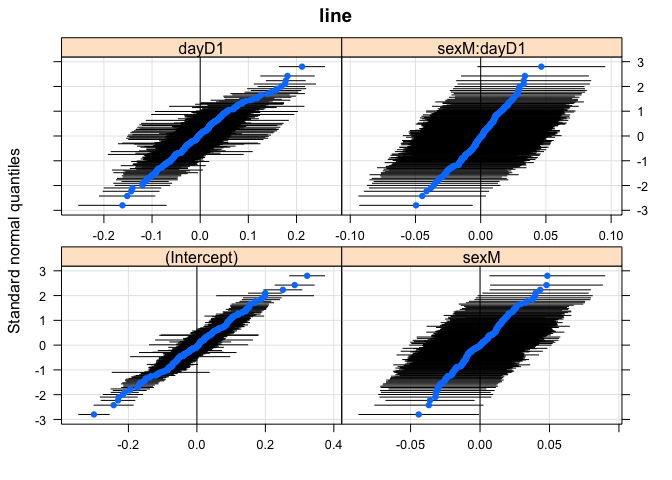
\includegraphics{_PreliminaryAnalysis_files/figure-latex/unnamed-chunk-56-1.pdf}
SSD1 has the highest correlation with female size variation

DOES IT MAKE SENSE TO COMPARE CORRELATIONS (is there a statistical
test), I want to know if female Day0 variation controls more SSD0 than
Day2 female size variation does for SSD2

We have shown that SSD in different condition changes, that in starved
conditions, we have a decrease in overall SSD, and that the variation of
SSD partly covariates with female size for SSD0 and SSD2. But the degree
of correlation varies? (how to test that?)

But if SSD changes under different conditions, that means that females
and males must have a different response to environmental changes, so we
should see a sex specific plasticity or SSP.

\#Section 3: SSP01 and SSP02 - Question 3.1: Is there SSP when we look
at fed vs starved flies? - Question 3.2: Does this SSP vary in the DGRP
flies? - Question 3.3: Is the variation in SSP due to a variation in SSD
in fed or starved flies? If SSP covaries with SSD0, that means that we
have variation in fed flies. If SSP covaries with starved flies, we have
variation in the reduction of flies size. - Question 3.4: If it is due
to SSD in either fed or starved flies, is it because the females vary
more or the males vary more in size? - Question 3.5: Does the variation
causing SSP (Question 3.4) is the same as the variation caused by SSD in
Question 1.3?

\#\#Question 3.1: Is there SSP when we look at fed vs starved flies?

\hypertarget{ssp01-between-fed-and-1-day-starved-flies}{%
\subsubsection{SSP01: between fed and 1 day starved
flies}\label{ssp01-between-fed-and-1-day-starved-flies}}

\begin{Shaded}
\begin{Highlighting}[]
\CommentTok{# use subset Day 1 and Day 0}
\NormalTok{df01<-}\KeywordTok{subset}\NormalTok{(df_sub, day}\OperatorTok{==}\StringTok{"D0"}\OperatorTok{|}\NormalTok{day}\OperatorTok{==}\StringTok{"D1"}\NormalTok{)}
\NormalTok{df01<-}\KeywordTok{na.omit}\NormalTok{(df01, }\DataTypeTok{cols=}\StringTok{"pupa"}\NormalTok{) }\CommentTok{#1447  rows}

\NormalTok{SSP01_test<-}\KeywordTok{lmer}\NormalTok{(pupa}\OperatorTok{~}\NormalTok{sex}\OperatorTok{*}\NormalTok{day}\OperatorTok{+}\NormalTok{(}\DecValTok{1}\OperatorTok{|}\NormalTok{line)}\OperatorTok{+}\NormalTok{(}\DecValTok{1}\OperatorTok{|}\NormalTok{block), }\DataTypeTok{REML=}\OtherTok{TRUE}\NormalTok{, }\DataTypeTok{data=}\NormalTok{df01) }\CommentTok{#random effect, there is variation in sex by line and there is variation in plasticity by line.}
\KeywordTok{summary}\NormalTok{(SSP01_test)}
\end{Highlighting}
\end{Shaded}

\begin{verbatim}
## Linear mixed model fit by REML. t-tests use Satterthwaite's method [
## lmerModLmerTest]
## Formula: pupa ~ sex * day + (1 | line) + (1 | block)
##    Data: df01
## 
## REML criterion at convergence: -17613.2
## 
## Scaled residuals: 
##     Min      1Q  Median      3Q     Max 
## -4.9221 -0.6382  0.0577  0.6666  4.1394 
## 
## Random effects:
##  Groups   Name        Variance Std.Dev.
##  line     (Intercept) 0.009614 0.09805 
##  block    (Intercept) 0.001823 0.04269 
##  Residual             0.016434 0.12819 
## Number of obs: 14474, groups:  line, 195; block, 9
## 
## Fixed effects:
##               Estimate Std. Error         df t value Pr(>|t|)    
## (Intercept)  1.457e+01  1.617e-02  9.561e+00 900.844  < 2e-16 ***
## sexM        -9.310e-02  2.883e-03  1.428e+04 -32.296  < 2e-16 ***
## dayD1       -1.751e-01  3.238e-03  1.436e+04 -54.085  < 2e-16 ***
## sexM:dayD1   2.610e-02  4.342e-03  1.429e+04   6.012 1.88e-09 ***
## ---
## Signif. codes:  0 '***' 0.001 '**' 0.01 '*' 0.05 '.' 0.1 ' ' 1
## 
## Correlation of Fixed Effects:
##            (Intr) sexM   dayD1 
## sexM       -0.092              
## dayD1      -0.088  0.455       
## sexM:dayD1  0.061 -0.660 -0.698
\end{verbatim}

\begin{Shaded}
\begin{Highlighting}[]
\KeywordTok{Anova}\NormalTok{(SSP01_test)}
\end{Highlighting}
\end{Shaded}

\begin{verbatim}
## Analysis of Deviance Table (Type II Wald chisquare tests)
## 
## Response: pupa
##           Chisq Df Pr(>Chisq)    
## sex     1423.22  1  < 2.2e-16 ***
## day     4858.28  1  < 2.2e-16 ***
## sex:day   36.14  1  1.837e-09 ***
## ---
## Signif. codes:  0 '***' 0.001 '**' 0.01 '*' 0.05 '.' 0.1 ' ' 1
\end{verbatim}

\hypertarget{ssp02-between-fed-and-1-day-starved-flies}{%
\subsubsection{SSP02: between fed and 1 day starved
flies}\label{ssp02-between-fed-and-1-day-starved-flies}}

\begin{Shaded}
\begin{Highlighting}[]
\CommentTok{# use subset Day 1 and Day 0}
\NormalTok{df02<-}\KeywordTok{subset}\NormalTok{(df, day}\OperatorTok{==}\StringTok{"D0"}\OperatorTok{|}\NormalTok{day}\OperatorTok{==}\StringTok{"D2"}\NormalTok{)}
\NormalTok{df02<-}\KeywordTok{na.omit}\NormalTok{(df02, }\DataTypeTok{cols=}\StringTok{"pupa"}\NormalTok{) }\CommentTok{#10738 rows}
\NormalTok{SSP02_test<-}\KeywordTok{lmer}\NormalTok{(pupa}\OperatorTok{~}\NormalTok{sex}\OperatorTok{*}\NormalTok{day}\OperatorTok{+}\NormalTok{(}\DecValTok{1}\OperatorTok{|}\NormalTok{line)}\OperatorTok{+}\NormalTok{(}\DecValTok{1}\OperatorTok{|}\NormalTok{block), }\DataTypeTok{REML=}\OtherTok{TRUE}\NormalTok{, }\DataTypeTok{data=}\NormalTok{df02) }\CommentTok{#random effect, there is variation in sex by line and there is variation in plasticity by line.}
\KeywordTok{summary}\NormalTok{(SSP02_test)}
\end{Highlighting}
\end{Shaded}

\begin{verbatim}
## Linear mixed model fit by REML. t-tests use Satterthwaite's method [
## lmerModLmerTest]
## Formula: pupa ~ sex * day + (1 | line) + (1 | block)
##    Data: df02
## 
## REML criterion at convergence: -13989.1
## 
## Scaled residuals: 
##     Min      1Q  Median      3Q     Max 
## -5.1457 -0.6418  0.0686  0.6856  3.4675 
## 
## Random effects:
##  Groups   Name        Variance Std.Dev.
##  line     (Intercept) 0.009720 0.09859 
##  block    (Intercept) 0.003069 0.05540 
##  Residual             0.014884 0.12200 
## Number of obs: 10738, groups:  line, 189; block, 9
## 
## Fixed effects:
##               Estimate Std. Error         df t value Pr(>|t|)    
## (Intercept)  1.457e+01  2.007e-02  9.093e+00 725.743   <2e-16 ***
## sexM        -9.395e-02  2.752e-03  1.056e+04 -34.138   <2e-16 ***
## dayD2       -2.528e-01  4.330e-03  1.064e+04 -58.387   <2e-16 ***
## sexM:dayD2   1.276e-02  5.533e-03  1.056e+04   2.306   0.0211 *  
## ---
## Signif. codes:  0 '***' 0.001 '**' 0.01 '*' 0.05 '.' 0.1 ' ' 1
## 
## Correlation of Fixed Effects:
##            (Intr) sexM   dayD2 
## sexM       -0.070              
## dayD2      -0.050  0.313       
## sexM:dayD2  0.035 -0.493 -0.647
\end{verbatim}

\begin{Shaded}
\begin{Highlighting}[]
\KeywordTok{Anova}\NormalTok{(SSP02_test)}
\end{Highlighting}
\end{Shaded}

\begin{verbatim}
## Analysis of Deviance Table (Type II Wald chisquare tests)
## 
## Response: pupa
##             Chisq Df Pr(>Chisq)    
## sex     1438.9486  1    < 2e-16 ***
## day     5562.9346  1    < 2e-16 ***
## sex:day    5.3168  1    0.02112 *  
## ---
## Signif. codes:  0 '***' 0.001 '**' 0.01 '*' 0.05 '.' 0.1 ' ' 1
\end{verbatim}

\#\#Question 3.2: Does this SSP vary in the DGRP flies? \#\#\# SSP01

\begin{Shaded}
\begin{Highlighting}[]
\CommentTok{# we want to compare effect of sex and day of starvation on pupal size. I am using df01, subset off data day 0 and day1}

\NormalTok{model2<-}\KeywordTok{lmer}\NormalTok{(pupa}\OperatorTok{~}\NormalTok{sex}\OperatorTok{*}\NormalTok{day}\OperatorTok{+}\NormalTok{(}\DecValTok{1}\OperatorTok{|}\NormalTok{line)}\OperatorTok{+}\NormalTok{(}\DecValTok{1}\OperatorTok{|}\NormalTok{block), }\DataTypeTok{data=}\NormalTok{df01)}
\NormalTok{model1<-}\KeywordTok{lmer}\NormalTok{(pupa}\OperatorTok{~}\NormalTok{sex}\OperatorTok{*}\NormalTok{day}\OperatorTok{+}\NormalTok{(sex}\OperatorTok{+}\NormalTok{day}\OperatorTok{|}\NormalTok{line)}\OperatorTok{+}\NormalTok{(}\DecValTok{1}\OperatorTok{|}\NormalTok{block), }\DataTypeTok{data=}\NormalTok{df01)}
\KeywordTok{anova}\NormalTok{(model1,model2)}
\end{Highlighting}
\end{Shaded}

\begin{verbatim}
## Data: df01
## Models:
## model2: pupa ~ sex * day + (1 | line) + (1 | block)
## model1: pupa ~ sex * day + (sex + day | line) + (1 | block)
##        npar    AIC    BIC logLik deviance  Chisq Df Pr(>Chisq)    
## model2    7 -17635 -17582 8824.7   -17649                         
## model1   12 -18490 -18399 9256.9   -18514 864.43  5  < 2.2e-16 ***
## ---
## Signif. codes:  0 '***' 0.001 '**' 0.01 '*' 0.05 '.' 0.1 ' ' 1
\end{verbatim}

Model 1 is better.

\hypertarget{do-a-lrt-3}{%
\subsubsection{Do a LRT}\label{do-a-lrt-3}}

How many parameters for each models

\begin{Shaded}
\begin{Highlighting}[]
\NormalTok{(}\KeywordTok{AIC}\NormalTok{(model1) }\OperatorTok{-}\StringTok{ }\KeywordTok{REMLcrit}\NormalTok{(model1))}\OperatorTok{/}\DecValTok{2} \CommentTok{# # of parameters the model "thinks" are being estimated}
\end{Highlighting}
\end{Shaded}

\begin{verbatim}
## [1] 12
\end{verbatim}

\begin{Shaded}
\begin{Highlighting}[]
\NormalTok{(}\KeywordTok{AIC}\NormalTok{(model2) }\OperatorTok{-}\StringTok{ }\KeywordTok{REMLcrit}\NormalTok{(model2))}\OperatorTok{/}\DecValTok{2} \CommentTok{# # of parameters the model "thinks" are being estimated}
\end{Highlighting}
\end{Shaded}

\begin{verbatim}
## [1] 7
\end{verbatim}

So lme4/lmer is treating model 1 as having five more parameters than
model2.

\begin{Shaded}
\begin{Highlighting}[]
\NormalTok{LR.model <-}\StringTok{  }\OperatorTok{-}\KeywordTok{as.numeric}\NormalTok{(}\KeywordTok{REMLcrit}\NormalTok{(model1) }\OperatorTok{-}\StringTok{ }\KeywordTok{REMLcrit}\NormalTok{(model2))}
\NormalTok{LR.model}
\end{Highlighting}
\end{Shaded}

\begin{verbatim}
## [1] 866.7934
\end{verbatim}

\begin{Shaded}
\begin{Highlighting}[]
\KeywordTok{nlevels}\NormalTok{(df01}\OperatorTok{$}\NormalTok{line)}
\end{Highlighting}
\end{Shaded}

\begin{verbatim}
## [1] 0
\end{verbatim}

\begin{Shaded}
\begin{Highlighting}[]
\KeywordTok{pchisq}\NormalTok{(}\DataTypeTok{q =}\NormalTok{ LR.model, }\DataTypeTok{df=}\DecValTok{5}\NormalTok{, }\DataTypeTok{lower=}\NormalTok{F)}
\end{Highlighting}
\end{Shaded}

\begin{verbatim}
## [1] 4.086886e-185
\end{verbatim}

\begin{Shaded}
\begin{Highlighting}[]
\KeywordTok{pchisq}\NormalTok{(}\DataTypeTok{q =}\NormalTok{ LR.model, }\DataTypeTok{df=}\KeywordTok{nlevels}\NormalTok{(df01}\OperatorTok{$}\NormalTok{line), }\DataTypeTok{lower=}\NormalTok{F)}
\end{Highlighting}
\end{Shaded}

\begin{verbatim}
## [1] 0
\end{verbatim}

\hypertarget{parametric-boostrap-3}{%
\subsubsection{Parametric boostrap}\label{parametric-boostrap-3}}

Finally, we can conduct a parametric bootstrap to compare the two
models.

\hypertarget{finally-using-bayesian-analysis-3}{%
\subsubsection{Finally using Bayesian
Analysis}\label{finally-using-bayesian-analysis-3}}

\#\#NB: did not run before need to change the model

\begin{Shaded}
\begin{Highlighting}[]
\CommentTok{#prior.2 <-list(R=list(V=0.01, nu=0.002), }
  \CommentTok{#             G=list(G1=list(V=0.01*diag(1), nu=0.002),}
   \CommentTok{#                   G2=list(V=0.01*diag(2), nu=0.002)))}

\CommentTok{#model1M.MCMC <- MCMCglmm(pupa ~ 1 + sex, #is this right for SSP?}
  \CommentTok{#random=~block + us(1 + sex):line,}
  \CommentTok{#prior = prior.2, burnin = 5000, nitt = 20000, thin = 10,}
  \CommentTok{#verbose = F, pr = T,}
  \CommentTok{#data=df01)}
\CommentTok{#summary(model1M.MCMC)}
\end{Highlighting}
\end{Shaded}

\hypertarget{post-model-1-fitting-check-3}{%
\subsubsection{Post model 1 fitting
check}\label{post-model-1-fitting-check-3}}

\hypertarget{residual-distribution-3}{%
\paragraph{Residual distribution}\label{residual-distribution-3}}

\begin{Shaded}
\begin{Highlighting}[]
\NormalTok{res_model1=}\KeywordTok{residuals}\NormalTok{(model1)}
\end{Highlighting}
\end{Shaded}

\hypertarget{model-1-residual-distribution-3}{%
\paragraph{Model 1 residual
distribution}\label{model-1-residual-distribution-3}}

\begin{Shaded}
\begin{Highlighting}[]
\KeywordTok{plot}\NormalTok{(model1)}
\end{Highlighting}
\end{Shaded}

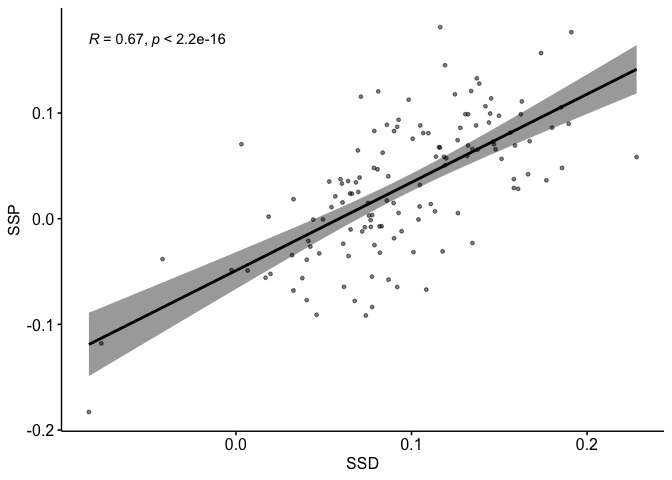
\includegraphics{_PreliminaryAnalysis_files/figure-latex/unnamed-chunk-66-1.pdf}

\hypertarget{qq-plot-3}{%
\paragraph{QQ plot}\label{qq-plot-3}}

\begin{Shaded}
\begin{Highlighting}[]
\KeywordTok{require}\NormalTok{(ggpubr)}
\KeywordTok{ggqqplot}\NormalTok{(res_model1)}
\end{Highlighting}
\end{Shaded}

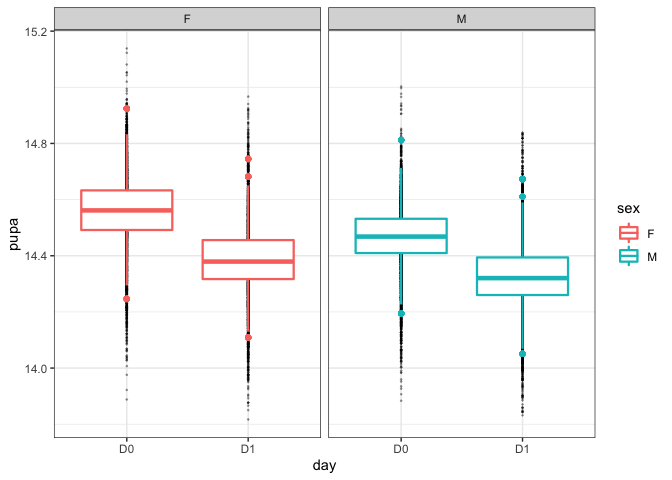
\includegraphics{_PreliminaryAnalysis_files/figure-latex/unnamed-chunk-67-1.pdf}

\hypertarget{random-effect-plot-3}{%
\paragraph{Random effect plot}\label{random-effect-plot-3}}

\begin{Shaded}
\begin{Highlighting}[]
\KeywordTok{qqmath}\NormalTok{(}\KeywordTok{ranef}\NormalTok{(model1))}
\end{Highlighting}
\end{Shaded}

\begin{verbatim}
## $line
\end{verbatim}

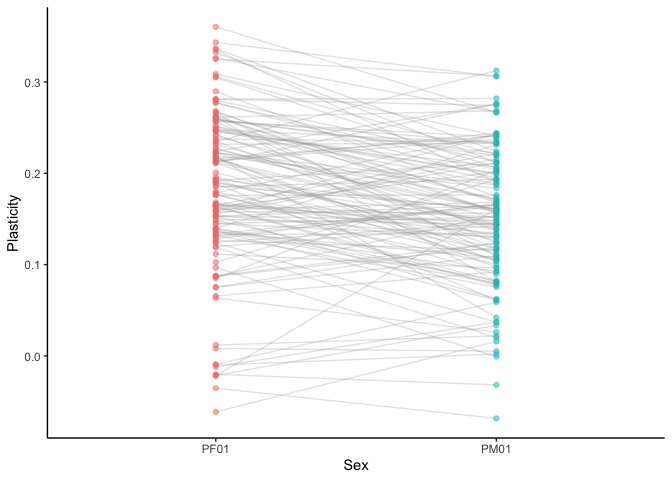
\includegraphics{_PreliminaryAnalysis_files/figure-latex/unnamed-chunk-68-1.pdf}

\begin{verbatim}
## 
## $block
\end{verbatim}

\includegraphics{_PreliminaryAnalysis_files/figure-latex/unnamed-chunk-68-2.pdf}
We have two plots, one for line and one for block

\hypertarget{ssp02}{%
\subsubsection{SSP02}\label{ssp02}}

\begin{Shaded}
\begin{Highlighting}[]
\CommentTok{# we want to compare effect of sex and day of starvation on pupal size. I am using df02, subset of data by day 0 and day 2}
\NormalTok{model2<-}\KeywordTok{lmer}\NormalTok{(pupa}\OperatorTok{~}\NormalTok{sex}\OperatorTok{*}\NormalTok{day}\OperatorTok{+}\NormalTok{(}\DecValTok{1}\OperatorTok{|}\NormalTok{line)}\OperatorTok{+}\NormalTok{(}\DecValTok{1}\OperatorTok{|}\NormalTok{block), }\DataTypeTok{data=}\NormalTok{df02)}
\NormalTok{model1<-}\KeywordTok{lmer}\NormalTok{(pupa}\OperatorTok{~}\NormalTok{sex}\OperatorTok{*}\NormalTok{day}\OperatorTok{+}\NormalTok{(sex}\OperatorTok{*}\NormalTok{day}\OperatorTok{|}\NormalTok{line)}\OperatorTok{+}\NormalTok{(}\DecValTok{1}\OperatorTok{|}\NormalTok{block), }\DataTypeTok{data=}\NormalTok{df02)}
\KeywordTok{anova}\NormalTok{(model1,model2)}
\end{Highlighting}
\end{Shaded}

\begin{verbatim}
## Data: df02
## Models:
## model2: pupa ~ sex * day + (1 | line) + (1 | block)
## model1: pupa ~ sex * day + (sex * day | line) + (1 | block)
##        npar    AIC    BIC logLik deviance  Chisq Df Pr(>Chisq)    
## model2    7 -14010 -13958 7011.7   -14024                         
## model1   16 -14905 -14788 7468.5   -14937 913.55  9  < 2.2e-16 ***
## ---
## Signif. codes:  0 '***' 0.001 '**' 0.01 '*' 0.05 '.' 0.1 ' ' 1
\end{verbatim}

Model 1 is better here.

\hypertarget{do-a-lrt-4}{%
\subsubsection{Do a LRT}\label{do-a-lrt-4}}

How many parameters for each models

\begin{Shaded}
\begin{Highlighting}[]
\NormalTok{(}\KeywordTok{AIC}\NormalTok{(model1) }\OperatorTok{-}\StringTok{ }\KeywordTok{REMLcrit}\NormalTok{(model1))}\OperatorTok{/}\DecValTok{2} \CommentTok{# # of parameters the model "thinks" are being estimated}
\end{Highlighting}
\end{Shaded}

\begin{verbatim}
## [1] 16
\end{verbatim}

\begin{Shaded}
\begin{Highlighting}[]
\NormalTok{(}\KeywordTok{AIC}\NormalTok{(model2) }\OperatorTok{-}\StringTok{ }\KeywordTok{REMLcrit}\NormalTok{(model2))}\OperatorTok{/}\DecValTok{2} \CommentTok{# # of parameters the model "thinks" are being estimated}
\end{Highlighting}
\end{Shaded}

\begin{verbatim}
## [1] 7
\end{verbatim}

So lme4/lmer is treating model 1 as having nine more parameters than
model2.

\begin{Shaded}
\begin{Highlighting}[]
\NormalTok{LR.model <-}\StringTok{  }\OperatorTok{-}\KeywordTok{as.numeric}\NormalTok{(}\KeywordTok{REMLcrit}\NormalTok{(model1) }\OperatorTok{-}\StringTok{ }\KeywordTok{REMLcrit}\NormalTok{(model2))}
\NormalTok{LR.model}
\end{Highlighting}
\end{Shaded}

\begin{verbatim}
## [1] 916.3482
\end{verbatim}

\begin{Shaded}
\begin{Highlighting}[]
\KeywordTok{nlevels}\NormalTok{(df02}\OperatorTok{$}\NormalTok{line)}
\end{Highlighting}
\end{Shaded}

\begin{verbatim}
## [1] 0
\end{verbatim}

\begin{Shaded}
\begin{Highlighting}[]
\KeywordTok{pchisq}\NormalTok{(}\DataTypeTok{q =}\NormalTok{ LR.model, }\DataTypeTok{df=}\DecValTok{9}\NormalTok{, }\DataTypeTok{lower=}\NormalTok{F)}
\end{Highlighting}
\end{Shaded}

\begin{verbatim}
## [1] 1.856931e-191
\end{verbatim}

\begin{Shaded}
\begin{Highlighting}[]
\KeywordTok{pchisq}\NormalTok{(}\DataTypeTok{q =}\NormalTok{ LR.model, }\DataTypeTok{df=}\KeywordTok{nlevels}\NormalTok{(df02}\OperatorTok{$}\NormalTok{line), }\DataTypeTok{lower=}\NormalTok{F)}
\end{Highlighting}
\end{Shaded}

\begin{verbatim}
## [1] 0
\end{verbatim}

\hypertarget{parametric-boostrap-4}{%
\subsubsection{Parametric boostrap}\label{parametric-boostrap-4}}

Finally, we can conduct a parametric bootstrap to compare the two
models.

\hypertarget{finally-using-bayesian-analysis-4}{%
\subsubsection{Finally using Bayesian
Analysis}\label{finally-using-bayesian-analysis-4}}

\#did not run because need to update model

\begin{Shaded}
\begin{Highlighting}[]
\CommentTok{#prior.2 <-list(R=list(V=0.01, nu=0.002), }
 \CommentTok{#              G=list(G1=list(V=0.01*diag(1), nu=0.002),}
  \CommentTok{#                    G2=list(V=0.01*diag(2), nu=0.002)))}

\CommentTok{#model1M.MCMC <- MCMCglmm(pupa ~ 1 + sex, }
 \CommentTok{# random=~block + us(1 + sex):line,}
\CommentTok{#  prior = prior.2, burnin = 5000, nitt = 20000, thin = 10,}
 \CommentTok{# verbose = F, pr = T,}
\CommentTok{#  data=df02)}
\CommentTok{#summary(model1M.MCMC)}
\end{Highlighting}
\end{Shaded}

\hypertarget{post-model-1-fitting-check-4}{%
\subsubsection{Post model 1 fitting
check}\label{post-model-1-fitting-check-4}}

\hypertarget{residual-distribution-4}{%
\paragraph{Residual distribution}\label{residual-distribution-4}}

\begin{Shaded}
\begin{Highlighting}[]
\NormalTok{res_model1=}\KeywordTok{residuals}\NormalTok{(model1)}
\end{Highlighting}
\end{Shaded}

\hypertarget{model-1-residual-distribution-4}{%
\paragraph{Model 1 residual
distribution}\label{model-1-residual-distribution-4}}

\begin{Shaded}
\begin{Highlighting}[]
\KeywordTok{plot}\NormalTok{(model1)}
\end{Highlighting}
\end{Shaded}

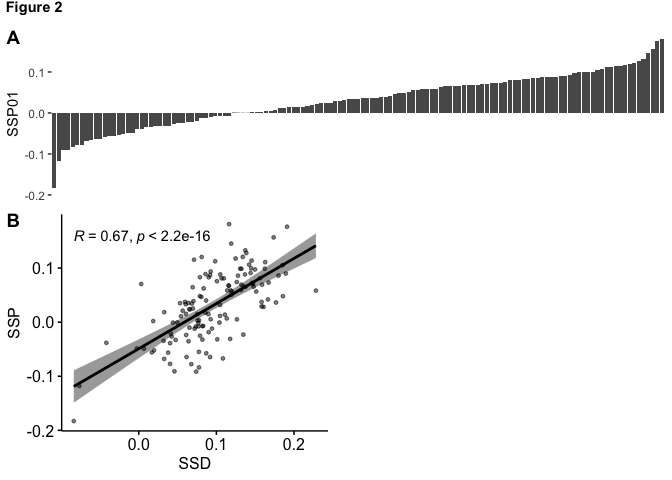
\includegraphics{_PreliminaryAnalysis_files/figure-latex/unnamed-chunk-75-1.pdf}

\hypertarget{qq-plot-4}{%
\paragraph{QQ plot}\label{qq-plot-4}}

\begin{Shaded}
\begin{Highlighting}[]
\KeywordTok{require}\NormalTok{(ggpubr)}
\KeywordTok{ggqqplot}\NormalTok{(res_model1)}
\end{Highlighting}
\end{Shaded}

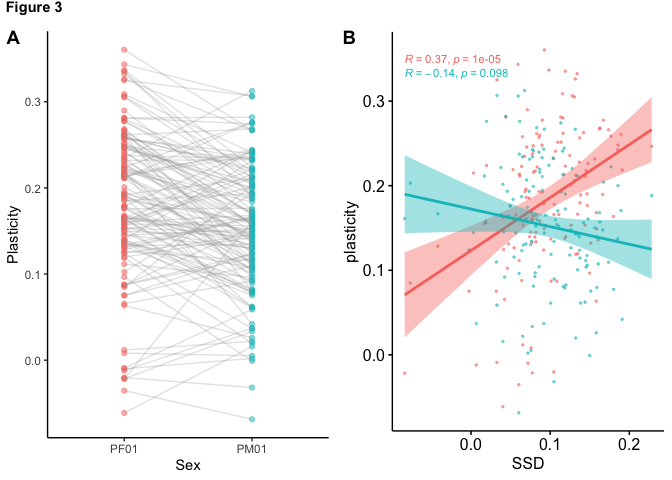
\includegraphics{_PreliminaryAnalysis_files/figure-latex/unnamed-chunk-76-1.pdf}

\hypertarget{random-effect-plot-4}{%
\paragraph{Random effect plot}\label{random-effect-plot-4}}

\begin{Shaded}
\begin{Highlighting}[]
\KeywordTok{qqmath}\NormalTok{(}\KeywordTok{ranef}\NormalTok{(model1))}
\end{Highlighting}
\end{Shaded}

\begin{verbatim}
## $line
\end{verbatim}

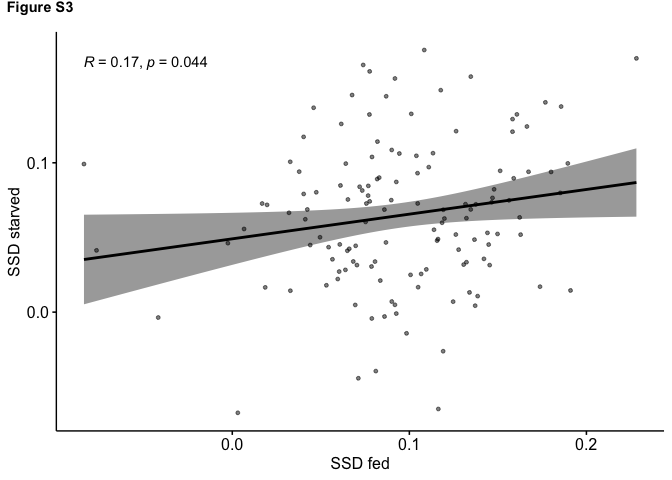
\includegraphics{_PreliminaryAnalysis_files/figure-latex/unnamed-chunk-77-1.pdf}

\begin{verbatim}
## 
## $block
\end{verbatim}

\includegraphics{_PreliminaryAnalysis_files/figure-latex/unnamed-chunk-77-2.pdf}
We have two plots, one for line and one for block

Answer 3.2: There is genetic variation in SSP if we compare fed flies
and starved flies. BUT need to check with Alex if my model is correct.

\#\#Question 3.3: Is the variation in SSP due to a variation in SSD in
fed or starved flies? Look at the correlation between SSP01, SSD0 and
SSD1 To calculate SSP, I first calculate the plasticity of female and
male and subtract the plasticity female-male

\begin{Shaded}
\begin{Highlighting}[]
\CommentTok{#calculate plasticity female}
\KeywordTok{head}\NormalTok{(df1)}
\end{Highlighting}
\end{Shaded}

\begin{verbatim}
## # A tibble: 6 x 10
## # Groups:   group [5]
##   id             line  block day   sex    wing   leg  pupa group    pupa_noblock
##   <chr>          <chr> <chr> <chr> <chr> <dbl> <dbl> <dbl> <chr>           <dbl>
## 1 317-B-1-F-7742 L317  B11   D1    F      13.7  13.4  13.8 L317_F_~       -0.607
## 2 911-B-1-M-096  L911  B7    D1    M      13.3  13.0  13.8 L911_M_~       -0.537
## 3 796-A-1-M-034  L796  B7    D1    M      13.6  13.6  13.8 L796_M_~       -0.526
## 4 105-A-1-M-7585 L105  B11   D1    M      13.5  13.4  13.8 L105_M_~       -0.581
## 5 105-B-1-M-7570 L105  B11   D1    M      13.5  13.2  13.8 L105_M_~       -0.579
## 6 861-B-1-M-101  L861  B7    D1    M      13.5  13.2  13.8 L861_M_~       -0.524
\end{verbatim}

\begin{Shaded}
\begin{Highlighting}[]
\NormalTok{df1F<-}\KeywordTok{subset}\NormalTok{(df1, sex}\OperatorTok{==}\StringTok{"F"}\NormalTok{)}
\KeywordTok{head}\NormalTok{(df1F)}
\end{Highlighting}
\end{Shaded}

\begin{verbatim}
## # A tibble: 6 x 10
## # Groups:   group [5]
##   id             line  block day   sex    wing   leg  pupa group    pupa_noblock
##   <chr>          <chr> <chr> <chr> <chr> <dbl> <dbl> <dbl> <chr>           <dbl>
## 1 317-B-1-F-7742 L317  B11   D1    F      13.7  13.4  13.8 L317_F_~       -0.607
## 2 595-B-1-F-104  L595  B6    D1    F      13.7  13.2  13.9 L595_F_~       -0.522
## 3 584-B-1-F-7029 L584  B11   D1    F      13.9  13.5  13.9 L584_F_~       -0.558
## 4 595-B-1-F-088  L595  B6    D1    F      13.6  13.2  13.9 L595_F_~       -0.496
## 5 505-A-1-F-648  L505  B12   D1    F      14.1  13.8  13.9 L505_F_~       -0.592
## 6 392-B-1-F-084  L392  B6    D1    F      13.9  13.7  13.9 L392_F_~       -0.495
\end{verbatim}

\begin{Shaded}
\begin{Highlighting}[]
\NormalTok{df1F_mean<-}\KeywordTok{aggregate}\NormalTok{(df1F[, }\DecValTok{10}\NormalTok{], }\KeywordTok{list}\NormalTok{(df1F}\OperatorTok{$}\NormalTok{line), mean)}
\KeywordTok{colnames}\NormalTok{(df1F_mean)<-}\KeywordTok{c}\NormalTok{(}\StringTok{"line"}\NormalTok{,}\StringTok{"pupaFmean_1"}\NormalTok{)}
\KeywordTok{head}\NormalTok{(df1F_mean)}
\end{Highlighting}
\end{Shaded}

\begin{verbatim}
##   line pupaFmean_1
## 1 L100  0.08515325
## 2 L101 -0.03520331
## 3 L105 -0.08479509
## 4 L109 -0.15244216
## 5 L129  0.04989262
## 6 L136 -0.09580059
\end{verbatim}

\begin{Shaded}
\begin{Highlighting}[]
\NormalTok{df0F<-}\KeywordTok{subset}\NormalTok{(df0, sex}\OperatorTok{==}\StringTok{"F"}\NormalTok{)}
\NormalTok{df0F_mean<-}\KeywordTok{aggregate}\NormalTok{(df0F[, }\DecValTok{10}\NormalTok{], }\KeywordTok{list}\NormalTok{(df0F}\OperatorTok{$}\NormalTok{line), mean)}
\KeywordTok{colnames}\NormalTok{(df0F_mean)<-}\KeywordTok{c}\NormalTok{(}\StringTok{"line"}\NormalTok{,}\StringTok{"pupaFmean_0"}\NormalTok{)}
\KeywordTok{head}\NormalTok{(df0F_mean)}
\end{Highlighting}
\end{Shaded}

\begin{verbatim}
##   line  pupaFmean_0
## 1 L100  0.256259113
## 2 L101  0.109003255
## 3 L105 -0.003621951
## 4 L109  0.063180232
## 5 L136  0.184305984
## 6 L138  0.207235102
\end{verbatim}

\begin{Shaded}
\begin{Highlighting}[]
\NormalTok{df2F<-}\KeywordTok{subset}\NormalTok{(df2, sex}\OperatorTok{==}\StringTok{"F"}\NormalTok{)}
\NormalTok{df2F_mean<-}\KeywordTok{aggregate}\NormalTok{(df2F[, }\DecValTok{10}\NormalTok{], }\KeywordTok{list}\NormalTok{(df2F}\OperatorTok{$}\NormalTok{line), mean)}
\KeywordTok{colnames}\NormalTok{(df2F_mean)<-}\KeywordTok{c}\NormalTok{(}\StringTok{"line"}\NormalTok{,}\StringTok{"pupaFmean_2"}\NormalTok{)}
\KeywordTok{head}\NormalTok{(df2F_mean)}
\end{Highlighting}
\end{Shaded}

\begin{verbatim}
##   line  pupaFmean_2
## 1 L153  0.208349100
## 2 L158  0.019870621
## 3 L195 -0.324207734
## 4 L229  0.025244072
## 5 L256 -0.051082781
## 6  L26 -0.002092585
\end{verbatim}

\begin{Shaded}
\begin{Highlighting}[]
\NormalTok{pupa_mean_F01<-}\KeywordTok{merge}\NormalTok{(}\DataTypeTok{x=}\NormalTok{df0F_mean, }\DataTypeTok{y=}\NormalTok{df1F_mean, }\DataTypeTok{by.x=}\StringTok{"line"}\NormalTok{, }\DataTypeTok{by.y=}\StringTok{"line"}\NormalTok{) }\CommentTok{#cannot merge all three treatment together or we loose data because less data at Day 2}
\KeywordTok{head}\NormalTok{(pupa_mean_F01) }\CommentTok{#151}
\end{Highlighting}
\end{Shaded}

\begin{verbatim}
##   line  pupaFmean_0  pupaFmean_1
## 1 L100  0.256259113  0.085153254
## 2 L101  0.109003255 -0.035203315
## 3 L105 -0.003621951 -0.084795090
## 4 L109  0.063180232 -0.152442163
## 5 L136  0.184305984 -0.095800591
## 6 L138  0.207235102 -0.009467483
\end{verbatim}

\begin{Shaded}
\begin{Highlighting}[]
\CommentTok{#for SSP02}
\NormalTok{pupa_mean_F02<-}\KeywordTok{merge}\NormalTok{(}\DataTypeTok{x=}\NormalTok{df0F_mean, }\DataTypeTok{y=}\NormalTok{df2F_mean, }\DataTypeTok{by.x=}\StringTok{"line"}\NormalTok{, }\DataTypeTok{by.y=}\StringTok{"line"}\NormalTok{)}
\KeywordTok{head}\NormalTok{(pupa_mean_F02) }\CommentTok{#66 lines}
\end{Highlighting}
\end{Shaded}

\begin{verbatim}
##   line pupaFmean_0  pupaFmean_2
## 1 L158   0.4372961  0.019870621
## 2 L195   0.2585795 -0.324207734
## 3 L229   0.2342914  0.025244072
## 4 L256   0.1506149 -0.051082781
## 5  L26   0.2132552 -0.002092585
## 6  L28   0.2039808  0.092029050
\end{verbatim}

\begin{Shaded}
\begin{Highlighting}[]
\NormalTok{pupa_mean_F01}\OperatorTok{$}\NormalTok{PF01<-pupa_mean_F01}\OperatorTok{$}\NormalTok{pupaFmean_}\DecValTok{0}\OperatorTok{-}\NormalTok{pupa_mean_F01}\OperatorTok{$}\NormalTok{pupaFmean_}\DecValTok{1} \CommentTok{#calculating plast female 01}
\NormalTok{pupa_mean_F02}\OperatorTok{$}\NormalTok{PF02<-pupa_mean_F02}\OperatorTok{$}\NormalTok{pupaFmean_}\DecValTok{0}\OperatorTok{-}\NormalTok{pupa_mean_F02}\OperatorTok{$}\NormalTok{pupaFmean_}\DecValTok{2} \CommentTok{#calculating plast female 02}

\NormalTok{plastF01<-pupa_mean_F01 }
\NormalTok{plastF02<-pupa_mean_F02}
\end{Highlighting}
\end{Shaded}

\begin{Shaded}
\begin{Highlighting}[]
\CommentTok{#calculate plasticity male}
\KeywordTok{head}\NormalTok{(df1)}
\end{Highlighting}
\end{Shaded}

\begin{verbatim}
## # A tibble: 6 x 10
## # Groups:   group [5]
##   id             line  block day   sex    wing   leg  pupa group    pupa_noblock
##   <chr>          <chr> <chr> <chr> <chr> <dbl> <dbl> <dbl> <chr>           <dbl>
## 1 317-B-1-F-7742 L317  B11   D1    F      13.7  13.4  13.8 L317_F_~       -0.607
## 2 911-B-1-M-096  L911  B7    D1    M      13.3  13.0  13.8 L911_M_~       -0.537
## 3 796-A-1-M-034  L796  B7    D1    M      13.6  13.6  13.8 L796_M_~       -0.526
## 4 105-A-1-M-7585 L105  B11   D1    M      13.5  13.4  13.8 L105_M_~       -0.581
## 5 105-B-1-M-7570 L105  B11   D1    M      13.5  13.2  13.8 L105_M_~       -0.579
## 6 861-B-1-M-101  L861  B7    D1    M      13.5  13.2  13.8 L861_M_~       -0.524
\end{verbatim}

\begin{Shaded}
\begin{Highlighting}[]
\NormalTok{df1M<-}\KeywordTok{subset}\NormalTok{(df1, sex}\OperatorTok{==}\StringTok{"M"}\NormalTok{)}
\NormalTok{df1M_mean<-}\KeywordTok{aggregate}\NormalTok{(df1M[, }\DecValTok{10}\NormalTok{], }\KeywordTok{list}\NormalTok{(df1M}\OperatorTok{$}\NormalTok{line), mean)}
\KeywordTok{colnames}\NormalTok{(df1M_mean)<-}\KeywordTok{c}\NormalTok{(}\StringTok{"line"}\NormalTok{,}\StringTok{"pupaMmean_1"}\NormalTok{)}
\KeywordTok{head}\NormalTok{(df1M_mean)}
\end{Highlighting}
\end{Shaded}

\begin{verbatim}
##   line pupaMmean_1
## 1 L100  0.06014172
## 2 L101 -0.10079021
## 3 L105 -0.25153763
## 4 L109 -0.25892157
## 5 L129 -0.03625669
## 6 L136 -0.14308417
\end{verbatim}

\begin{Shaded}
\begin{Highlighting}[]
\NormalTok{df0M<-}\KeywordTok{subset}\NormalTok{(df0, sex}\OperatorTok{==}\StringTok{"M"}\NormalTok{)}
\NormalTok{df0M_mean<-}\KeywordTok{aggregate}\NormalTok{(df0M[, }\DecValTok{10}\NormalTok{], }\KeywordTok{list}\NormalTok{(df0M}\OperatorTok{$}\NormalTok{line), mean)}
\KeywordTok{colnames}\NormalTok{(df0M_mean)<-}\KeywordTok{c}\NormalTok{(}\StringTok{"line"}\NormalTok{,}\StringTok{"pupaMmean_0"}\NormalTok{)}
\KeywordTok{head}\NormalTok{(df0M_mean)}
\end{Highlighting}
\end{Shaded}

\begin{verbatim}
##   line pupaMmean_0
## 1 L100  0.11768444
## 2 L101  0.08961544
## 3 L105 -0.05341221
## 4 L109 -0.02019754
## 5 L136  0.06867247
## 6 L138  0.12057467
\end{verbatim}

\begin{Shaded}
\begin{Highlighting}[]
\NormalTok{df2M<-}\KeywordTok{subset}\NormalTok{(df2, sex}\OperatorTok{==}\StringTok{"M"}\NormalTok{)}
\NormalTok{df2M_mean<-}\KeywordTok{aggregate}\NormalTok{(df2M[, }\DecValTok{10}\NormalTok{], }\KeywordTok{list}\NormalTok{(df2M}\OperatorTok{$}\NormalTok{line), mean)}
\KeywordTok{colnames}\NormalTok{(df2M_mean)<-}\KeywordTok{c}\NormalTok{(}\StringTok{"line"}\NormalTok{,}\StringTok{"pupaMmean_2"}\NormalTok{)}
\KeywordTok{head}\NormalTok{(df2M_mean)}
\end{Highlighting}
\end{Shaded}

\begin{verbatim}
##   line pupaMmean_2
## 1 L100 -0.23292373
## 2 L153  0.08699819
## 3 L158 -0.07201030
## 4 L177 -0.35313746
## 5 L189 -0.30536655
## 6 L229 -0.17136726
\end{verbatim}

\begin{Shaded}
\begin{Highlighting}[]
\NormalTok{pupa_mean_M01<-}\KeywordTok{merge}\NormalTok{(}\DataTypeTok{x=}\NormalTok{df0M_mean, }\DataTypeTok{y=}\NormalTok{df1M_mean, }\DataTypeTok{by.x=}\StringTok{"line"}\NormalTok{, }\DataTypeTok{by.y=}\StringTok{"line"}\NormalTok{) }\CommentTok{#cannot merge all three treatment together or we loose data because less data at Day 2}
\KeywordTok{head}\NormalTok{(pupa_mean_F01) }\CommentTok{#151}
\end{Highlighting}
\end{Shaded}

\begin{verbatim}
##   line  pupaFmean_0  pupaFmean_1       PF01
## 1 L100  0.256259113  0.085153254 0.17110586
## 2 L101  0.109003255 -0.035203315 0.14420657
## 3 L105 -0.003621951 -0.084795090 0.08117314
## 4 L109  0.063180232 -0.152442163 0.21562240
## 5 L136  0.184305984 -0.095800591 0.28010657
## 6 L138  0.207235102 -0.009467483 0.21670258
\end{verbatim}

\begin{Shaded}
\begin{Highlighting}[]
\NormalTok{pupa_mean_M02<-}\KeywordTok{merge}\NormalTok{(}\DataTypeTok{x=}\NormalTok{df0M_mean, }\DataTypeTok{y=}\NormalTok{df2M_mean, }\DataTypeTok{by.x=}\StringTok{"line"}\NormalTok{, }\DataTypeTok{by.y=}\StringTok{"line"}\NormalTok{)}
\KeywordTok{head}\NormalTok{(pupa_mean_M02) }\CommentTok{#66 lines}
\end{Highlighting}
\end{Shaded}

\begin{verbatim}
##   line pupaMmean_0 pupaMmean_2
## 1 L100  0.11768444 -0.23292373
## 2 L153  0.17209388  0.08699819
## 3 L158  0.29326145 -0.07201030
## 4 L177 -0.02499460 -0.35313746
## 5 L189  0.08990092 -0.30536655
## 6 L229  0.10297417 -0.17136726
\end{verbatim}

\begin{Shaded}
\begin{Highlighting}[]
\NormalTok{pupa_mean_M01}\OperatorTok{$}\NormalTok{PM01<-pupa_mean_M01}\OperatorTok{$}\NormalTok{pupaMmean_}\DecValTok{0}\OperatorTok{-}\NormalTok{pupa_mean_M01}\OperatorTok{$}\NormalTok{pupaMmean_}\DecValTok{1} \CommentTok{#calculating SSP01}
\NormalTok{pupa_mean_M02}\OperatorTok{$}\NormalTok{PM02<-pupa_mean_M02}\OperatorTok{$}\NormalTok{pupaMmean_}\DecValTok{0}\OperatorTok{-}\NormalTok{pupa_mean_M02}\OperatorTok{$}\NormalTok{pupaMmean_}\DecValTok{2} \CommentTok{#calculating SSP02}

\NormalTok{plastM01<-pupa_mean_M01 }
\NormalTok{plastM02<-pupa_mean_M02}
\end{Highlighting}
\end{Shaded}

\begin{Shaded}
\begin{Highlighting}[]
\CommentTok{#SSP01}

\NormalTok{pupa_SSP01<-}\KeywordTok{merge}\NormalTok{(}\DataTypeTok{x=}\NormalTok{plastF01, }\DataTypeTok{y=}\NormalTok{ plastM01, }\DataTypeTok{by.x=}\StringTok{"line"}\NormalTok{, }\DataTypeTok{by.y=}\StringTok{"line"}\NormalTok{) }\CommentTok{#merging male and female datasets}
\KeywordTok{head}\NormalTok{(pupa_SSP01)}
\end{Highlighting}
\end{Shaded}

\begin{verbatim}
##   line  pupaFmean_0  pupaFmean_1       PF01 pupaMmean_0 pupaMmean_1       PM01
## 1 L100  0.256259113  0.085153254 0.17110586  0.11768444  0.06014172 0.05754272
## 2 L101  0.109003255 -0.035203315 0.14420657  0.08961544 -0.10079021 0.19040565
## 3 L105 -0.003621951 -0.084795090 0.08117314 -0.05341221 -0.25153763 0.19812542
## 4 L109  0.063180232 -0.152442163 0.21562240 -0.02019754 -0.25892157 0.23872403
## 5 L136  0.184305984 -0.095800591 0.28010657  0.06867247 -0.14308417 0.21175665
## 6 L138  0.207235102 -0.009467483 0.21670258  0.12057467 -0.04318888 0.16376355
\end{verbatim}

\begin{Shaded}
\begin{Highlighting}[]
\KeywordTok{length}\NormalTok{(}\KeywordTok{unique}\NormalTok{(pupa_SSP01}\OperatorTok{$}\NormalTok{line)) }\CommentTok{#146 lines left}
\end{Highlighting}
\end{Shaded}

\begin{verbatim}
## [1] 146
\end{verbatim}

\begin{Shaded}
\begin{Highlighting}[]
\CommentTok{#SSP02}
\NormalTok{pupa_SSP02<-}\KeywordTok{merge}\NormalTok{(}\DataTypeTok{x=}\NormalTok{plastF02, }\DataTypeTok{y=}\NormalTok{ plastM02, }\DataTypeTok{by.x=}\StringTok{"line"}\NormalTok{, }\DataTypeTok{by.y=}\StringTok{"line"}\NormalTok{) }\CommentTok{#merging male and female datasets}
\KeywordTok{head}\NormalTok{(pupa_SSP02)}
\end{Highlighting}
\end{Shaded}

\begin{verbatim}
##   line pupaFmean_0  pupaFmean_2      PF02  pupaMmean_0  pupaMmean_2       PM02
## 1 L158  0.43729608  0.019870621 0.4174255  0.293261448 -0.072010303 0.36527175
## 2 L229  0.23429138  0.025244072 0.2090473  0.102974168 -0.171367258 0.27434143
## 3 L256  0.15061487 -0.051082781 0.2016977  0.090507203 -0.174299175 0.26480638
## 4  L26  0.21325524 -0.002092585 0.2153478  0.103814444 -0.104164760 0.20797920
## 5  L28  0.20398076  0.092029050 0.1119517  0.145080084 -0.003598201 0.14867829
## 6 L313  0.08642449 -0.117978446 0.2044029 -0.002395298 -0.096055488 0.09366019
\end{verbatim}

\begin{Shaded}
\begin{Highlighting}[]
\KeywordTok{length}\NormalTok{(}\KeywordTok{unique}\NormalTok{(pupa_SSP02}\OperatorTok{$}\NormalTok{line)) }\CommentTok{#55 lines left}
\end{Highlighting}
\end{Shaded}

\begin{verbatim}
## [1] 55
\end{verbatim}

\begin{Shaded}
\begin{Highlighting}[]
\CommentTok{#calculate SSP from the plasticity.}
\NormalTok{pupa_SSP01}\OperatorTok{$}\NormalTok{SSP01<-pupa_SSP01}\OperatorTok{$}\NormalTok{PF01}\OperatorTok{-}\NormalTok{pupa_SSP01}\OperatorTok{$}\NormalTok{PM01}

\NormalTok{pupa_SSP02}\OperatorTok{$}\NormalTok{SSP02<-pupa_SSP02}\OperatorTok{$}\NormalTok{PF02}\OperatorTok{-}\NormalTok{pupa_SSP02}\OperatorTok{$}\NormalTok{PM02}


\CommentTok{#calculating SSDs again to add them to the dataframe}
\NormalTok{pupa_SSP01}\OperatorTok{$}\NormalTok{SSD0<-pupa_SSP01}\OperatorTok{$}\NormalTok{pupaFmean_}\DecValTok{0}\OperatorTok{-}\NormalTok{pupa_SSP01}\OperatorTok{$}\NormalTok{pupaMmean_}\DecValTok{0}
\NormalTok{pupa_SSP01}\OperatorTok{$}\NormalTok{SSD1<-pupa_SSP01}\OperatorTok{$}\NormalTok{pupaFmean_}\DecValTok{1}\OperatorTok{-}\NormalTok{pupa_SSP01}\OperatorTok{$}\NormalTok{pupaMmean_}\DecValTok{1}


\NormalTok{pupa_SSP02}\OperatorTok{$}\NormalTok{SSD0<-pupa_SSP02}\OperatorTok{$}\NormalTok{pupaFmean_}\DecValTok{0}\OperatorTok{-}\NormalTok{pupa_SSP02}\OperatorTok{$}\NormalTok{pupaMmean_}\DecValTok{0}
\NormalTok{pupa_SSP02}\OperatorTok{$}\NormalTok{SSD2<-pupa_SSP02}\OperatorTok{$}\NormalTok{pupaFmean_}\DecValTok{2}\OperatorTok{-}\NormalTok{pupa_SSP02}\OperatorTok{$}\NormalTok{pupaMmean_}\DecValTok{2}
\end{Highlighting}
\end{Shaded}

\hypertarget{correlation-between-ssp-and-ssds}{%
\paragraph{Correlation between SSP and
SSDs}\label{correlation-between-ssp-and-ssds}}

\hypertarget{ssp01-ssd0-and-ssd1}{%
\subparagraph{SSP01, SSD0 and SSD1}\label{ssp01-ssd0-and-ssd1}}

Is SSD0 or 1 covarying with SSP01?

\begin{Shaded}
\begin{Highlighting}[]
\CommentTok{#use pupa_SSP01 }
\KeywordTok{head}\NormalTok{(pupa_SSP01)}
\end{Highlighting}
\end{Shaded}

\begin{verbatim}
##   line  pupaFmean_0  pupaFmean_1       PF01 pupaMmean_0 pupaMmean_1       PM01
## 1 L100  0.256259113  0.085153254 0.17110586  0.11768444  0.06014172 0.05754272
## 2 L101  0.109003255 -0.035203315 0.14420657  0.08961544 -0.10079021 0.19040565
## 3 L105 -0.003621951 -0.084795090 0.08117314 -0.05341221 -0.25153763 0.19812542
## 4 L109  0.063180232 -0.152442163 0.21562240 -0.02019754 -0.25892157 0.23872403
## 5 L136  0.184305984 -0.095800591 0.28010657  0.06867247 -0.14308417 0.21175665
## 6 L138  0.207235102 -0.009467483 0.21670258  0.12057467 -0.04318888 0.16376355
##         SSP01       SSD0       SSD1
## 1  0.11356314 0.13857467 0.02501154
## 2 -0.04619908 0.01938781 0.06558689
## 3 -0.11695228 0.04979026 0.16674254
## 4 -0.02310163 0.08337778 0.10647941
## 5  0.06834993 0.11563351 0.04728358
## 6  0.05293904 0.08666043 0.03372139
\end{verbatim}

\begin{Shaded}
\begin{Highlighting}[]
\NormalTok{SSP01<-pupa_SSP01[}\KeywordTok{c}\NormalTok{(}\DecValTok{1}\NormalTok{,}\DecValTok{8}\OperatorTok{:}\DecValTok{10}\NormalTok{)]}
\KeywordTok{chart.Correlation}\NormalTok{(SSP01[}\DecValTok{2}\OperatorTok{:}\DecValTok{4}\NormalTok{],}
                   \DataTypeTok{method=}\StringTok{"pearson"}\NormalTok{,}
                   \DataTypeTok{histogram=}\OtherTok{TRUE}\NormalTok{,}
                   \DataTypeTok{pch=}\DecValTok{16}\NormalTok{)}
\end{Highlighting}
\end{Shaded}

\includegraphics{_PreliminaryAnalysis_files/figure-latex/unnamed-chunk-84-1.pdf}
The highest correlation is between SSD1 and SSP01, and it is a negative
correlation, which means that the higher SSP is, the more SSD decreases,
at lower food condition, one of the two sexes decreases in size more
than it increases in size in fed flies.

\hypertarget{correlation-ssp01-female-day-1-and-male-day-1-size}{%
\paragraph{Correlation SSP01, female Day 1 and male Day 1
size}\label{correlation-ssp01-female-day-1-and-male-day-1-size}}

\begin{Shaded}
\begin{Highlighting}[]
\KeywordTok{head}\NormalTok{(pupa_SSP01)}
\end{Highlighting}
\end{Shaded}

\begin{verbatim}
##   line  pupaFmean_0  pupaFmean_1       PF01 pupaMmean_0 pupaMmean_1       PM01
## 1 L100  0.256259113  0.085153254 0.17110586  0.11768444  0.06014172 0.05754272
## 2 L101  0.109003255 -0.035203315 0.14420657  0.08961544 -0.10079021 0.19040565
## 3 L105 -0.003621951 -0.084795090 0.08117314 -0.05341221 -0.25153763 0.19812542
## 4 L109  0.063180232 -0.152442163 0.21562240 -0.02019754 -0.25892157 0.23872403
## 5 L136  0.184305984 -0.095800591 0.28010657  0.06867247 -0.14308417 0.21175665
## 6 L138  0.207235102 -0.009467483 0.21670258  0.12057467 -0.04318888 0.16376355
##         SSP01       SSD0       SSD1
## 1  0.11356314 0.13857467 0.02501154
## 2 -0.04619908 0.01938781 0.06558689
## 3 -0.11695228 0.04979026 0.16674254
## 4 -0.02310163 0.08337778 0.10647941
## 5  0.06834993 0.11563351 0.04728358
## 6  0.05293904 0.08666043 0.03372139
\end{verbatim}

\begin{Shaded}
\begin{Highlighting}[]
\NormalTok{SSP01_size<-pupa_SSP01[,}\KeywordTok{c}\NormalTok{(}\DecValTok{1}\NormalTok{,}\DecValTok{3}\NormalTok{,}\DecValTok{6}\NormalTok{,}\DecValTok{8}\NormalTok{)]}
\KeywordTok{head}\NormalTok{(SSP01_size)}
\end{Highlighting}
\end{Shaded}

\begin{verbatim}
##   line  pupaFmean_1 pupaMmean_1       SSP01
## 1 L100  0.085153254  0.06014172  0.11356314
## 2 L101 -0.035203315 -0.10079021 -0.04619908
## 3 L105 -0.084795090 -0.25153763 -0.11695228
## 4 L109 -0.152442163 -0.25892157 -0.02310163
## 5 L136 -0.095800591 -0.14308417  0.06834993
## 6 L138 -0.009467483 -0.04318888  0.05293904
\end{verbatim}

\begin{Shaded}
\begin{Highlighting}[]
\KeywordTok{chart.Correlation}\NormalTok{(SSP01_size[}\DecValTok{2}\OperatorTok{:}\DecValTok{4}\NormalTok{],}
                   \DataTypeTok{method=}\StringTok{"pearson"}\NormalTok{,}
                   \DataTypeTok{histogram=}\OtherTok{TRUE}\NormalTok{,}
                   \DataTypeTok{pch=}\DecValTok{16}\NormalTok{)}
\end{Highlighting}
\end{Shaded}

\includegraphics{_PreliminaryAnalysis_files/figure-latex/unnamed-chunk-85-1.pdf}
There is almost no correlation between SSP01 and male and weak
correlation with female size in Day 1 starvation. That means that SSP01
covaries negatively with SSD01,(when the difference in plasticity is
higher, then sexual size dimorphism decreases) We assumed that this
covariation was created by the variation in female size in Day1, but it
does not explain it very strongly?

\hypertarget{do-we-have-the-same-trend-in-ssp02-ssd0-and-ssd2}{%
\subparagraph{Do we have the same trend in SSP02, SSD0 and
SSD2?}\label{do-we-have-the-same-trend-in-ssp02-ssd0-and-ssd2}}

\begin{Shaded}
\begin{Highlighting}[]
\KeywordTok{head}\NormalTok{(pupa_SSP02)}
\end{Highlighting}
\end{Shaded}

\begin{verbatim}
##   line pupaFmean_0  pupaFmean_2      PF02  pupaMmean_0  pupaMmean_2       PM02
## 1 L158  0.43729608  0.019870621 0.4174255  0.293261448 -0.072010303 0.36527175
## 2 L229  0.23429138  0.025244072 0.2090473  0.102974168 -0.171367258 0.27434143
## 3 L256  0.15061487 -0.051082781 0.2016977  0.090507203 -0.174299175 0.26480638
## 4  L26  0.21325524 -0.002092585 0.2153478  0.103814444 -0.104164760 0.20797920
## 5  L28  0.20398076  0.092029050 0.1119517  0.145080084 -0.003598201 0.14867829
## 6 L313  0.08642449 -0.117978446 0.2044029 -0.002395298 -0.096055488 0.09366019
##          SSP02       SSD0        SSD2
## 1  0.052153707 0.14403463  0.09188092
## 2 -0.065294122 0.13131721  0.19661133
## 3 -0.063108726 0.06010767  0.12321639
## 4  0.007368619 0.10944079  0.10207217
## 5 -0.036726573 0.05890068  0.09562725
## 6  0.110742750 0.08881979 -0.02192296
\end{verbatim}

\begin{Shaded}
\begin{Highlighting}[]
\NormalTok{SSP02<-pupa_SSP02[}\KeywordTok{c}\NormalTok{(}\DecValTok{1}\NormalTok{,}\DecValTok{8}\OperatorTok{:}\DecValTok{10}\NormalTok{)]}
\KeywordTok{chart.Correlation}\NormalTok{(SSP02[}\DecValTok{2}\OperatorTok{:}\DecValTok{4}\NormalTok{],}
                   \DataTypeTok{method=}\StringTok{"pearson"}\NormalTok{,}
                   \DataTypeTok{histogram=}\OtherTok{TRUE}\NormalTok{,}
                   \DataTypeTok{pch=}\DecValTok{16}\NormalTok{)}
\end{Highlighting}
\end{Shaded}

\includegraphics{_PreliminaryAnalysis_files/figure-latex/unnamed-chunk-86-1.pdf}
SSP02 correlates the most with SSD2 and negatively, same as we found
between SSP01 and SSD1.

If SSPs covary wit starved SSDs, that means that the variation in
starved flies is more important than the variation in fed flies.

\hypertarget{question-3.4-if-it-is-due-to-ssd-in-either-fed-or-starved-flies-is-it-because-the-females-vary-more-or-the-males-vary-more-in-size}{%
\subsubsection{Question 3.4: If it is due to SSD in either fed or
starved flies, is it because the females vary more or the males vary
more in
size?}\label{question-3.4-if-it-is-due-to-ssd-in-either-fed-or-starved-flies-is-it-because-the-females-vary-more-or-the-males-vary-more-in-size}}

SSP02 covaries negatively with SSD2, which sex at Day 2 contributes to
SSD2 variation?

\begin{Shaded}
\begin{Highlighting}[]
\NormalTok{pupa_SSP02}
\end{Highlighting}
\end{Shaded}

\begin{verbatim}
##    line pupaFmean_0   pupaFmean_2       PF02  pupaMmean_0  pupaMmean_2
## 1  L158  0.43729608  0.0198706211 0.41742546  0.293261448 -0.072010303
## 2  L229  0.23429138  0.0252440717 0.20904730  0.102974168 -0.171367258
## 3  L256  0.15061487 -0.0510827809 0.20169765  0.090507203 -0.174299175
## 4   L26  0.21325524 -0.0020925854 0.21534782  0.103814444 -0.104164760
## 5   L28  0.20398076  0.0920290502 0.11195171  0.145080084 -0.003598201
## 6  L313  0.08642449 -0.1179784463 0.20440294 -0.002395298 -0.096055488
## 7  L315  0.30293785 -0.1372958724 0.44023372  0.145529230 -0.227830626
## 8  L319  0.17859862 -0.1905172024 0.36911583  0.090651674 -0.263133001
## 9  L320  0.18484665 -0.0151649423 0.20001159  0.078848358 -0.092589150
## 10 L338  0.15236521 -0.2255686647 0.37793388  0.088267277 -0.212390102
## 11 L354  0.10981696 -0.0808734568 0.19069042  0.005193520 -0.178212569
## 12 L362  0.17320512 -0.0422510651 0.21545619  0.012206121 -0.147820521
## 13 L367  0.21814602 -0.2825281894 0.50067421  0.123797090 -0.320091371
## 14 L371  0.18457073 -0.2004012237 0.38497196  0.048186876 -0.253068519
## 15  L38  0.10201199 -0.0307460122 0.13275801  0.032082037 -0.116562063
## 16 L383  0.26737197 -0.0190385109 0.28641048  0.095273743 -0.178242643
## 17 L390  0.19038070 -0.0147332607 0.20511396  0.093444624 -0.076423444
## 18 L391  0.19599146 -0.2205041647 0.41649563  0.101175091 -0.191912421
## 19 L392  0.28258894 -0.1719153572 0.45450430  0.163500113 -0.223307799
## 20 L405  0.09478426 -0.2012851854 0.29606945  0.038221116 -0.271726019
## 21 L406  0.23856506 -0.0657860658 0.30435112  0.119267159 -0.136983977
## 22 L409  0.30142139 -0.0172878930 0.31870928  0.161496435 -0.096135443
## 23 L437  0.13203153 -0.0977846693 0.22981620  0.062946266 -0.184148632
## 24 L440  0.13414730 -0.1554390872 0.28958639  0.028737437 -0.241890393
## 25 L505  0.15253354  0.0429097802 0.10962376  0.066586851 -0.046799809
## 26 L509  0.40121807  0.2485134551 0.15270461  0.274667009  0.143144992
## 27 L513 -0.20290035 -0.2903689004 0.08746855 -0.272234090 -0.300403284
## 28 L530  0.20640556 -0.2497311785 0.45613674  0.037733741 -0.258857879
## 29 L566  0.12810337 -0.0735318015 0.20163517  0.061249054 -0.114252463
## 30 L596  0.06603903 -0.2030872174 0.26912625 -0.072147747 -0.285939676
## 31 L627  0.10449155 -0.0636625560 0.16815411  0.179427674 -0.101912163
## 32 L630  0.16589633 -0.0005452741 0.16644161  0.096365698 -0.083705399
## 33 L646  0.08716395 -0.0121977293 0.09936168  0.026929647 -0.096034716
## 34 L703  0.01369494 -0.2122686207 0.22596356 -0.081545357 -0.280064183
## 35 L705  0.25731513 -0.1351255876 0.39244071  0.163192102 -0.182334959
## 36 L727  0.20467130 -0.0033413430 0.20801264  0.095100072 -0.115717830
## 37 L730  0.27275697  0.1447091845 0.12804779  0.165089466  0.070755243
## 38 L732  0.18488205 -0.0052659063 0.19014796  0.047318738 -0.164331749
## 39 L786  0.06902687 -0.2229516599 0.29197853 -0.041058786 -0.381456201
## 40 L802  0.33796479 -0.0854357841 0.42340057  0.247923484 -0.159692046
## 41 L810  0.31384881  0.0376951127 0.27615370  0.212287719 -0.045968804
## 42 L818  0.10650083 -0.2296882300 0.33618906  0.008580925 -0.242228125
## 43 L821  0.12717223 -0.1137744961 0.24094673  0.045312129 -0.234764347
## 44 L822  0.18340762 -0.0169807339 0.20038836  0.135978797 -0.105745285
## 45 L837  0.05597500 -0.1138931961 0.16986820 -0.017649712 -0.140305873
## 46  L85  0.25991001 -0.0835950963 0.34350511  0.093214397 -0.197718003
## 47 L852  0.28175838 -0.2130209089 0.49477929  0.050683432 -0.266100892
## 48 L857  0.15907730 -0.1652272431 0.32430455  0.091410392 -0.221544321
## 49 L859  0.33345623 -0.1076108039 0.44106704  0.176179013 -0.232294681
## 50 L892  0.14789557 -0.1948029739 0.34269854  0.121359158 -0.171113704
## 51 L894  0.20528074  0.1200987491 0.08518199  0.108681338  0.040896105
## 52 L897  0.08225686 -0.2552249009 0.33748176  0.003705242 -0.255385553
## 53 L907  0.32403638  0.0151010709 0.30893531  0.177524054 -0.010220978
## 54  L91  0.27770924 -0.1265304597 0.40423970  0.135591338 -0.246215481
## 55 L911 -0.09329649 -0.3148649245 0.22156843 -0.123998060 -0.330165402
##          PM02        SSP02        SSD0          SSD2
## 1  0.36527175  0.052153707  0.14403463  0.0918809238
## 2  0.27434143 -0.065294122  0.13131721  0.1966113298
## 3  0.26480638 -0.063108726  0.06010767  0.1232163941
## 4  0.20797920  0.007368619  0.10944079  0.1020721748
## 5  0.14867829 -0.036726573  0.05890068  0.0956272516
## 6  0.09366019  0.110742750  0.08881979 -0.0219229586
## 7  0.37335986  0.066873864  0.15740862  0.0905347537
## 8  0.35378468  0.015331150  0.08794695  0.0726157989
## 9  0.17143751  0.028574086  0.10599829  0.0774242074
## 10 0.30065738  0.077276499  0.06409794 -0.0131785622
## 11 0.18340609  0.007284330  0.10462344  0.0973391121
## 12 0.16002664  0.055429545  0.16099900  0.1055694556
## 13 0.44388846  0.056785751  0.09434893  0.0375631812
## 14 0.30125540  0.083716563  0.13638386  0.0526672950
## 15 0.14864410 -0.015886095  0.06992996  0.0858160511
## 16 0.27351639  0.012894095  0.17209823  0.1592041318
## 17 0.16986807  0.035245894  0.09693608  0.0616901830
## 18 0.29308751  0.123408117  0.09481637 -0.0285917437
## 19 0.38680791  0.067696389  0.11908883  0.0513924419
## 20 0.30994714 -0.013877686  0.05656315  0.0704408335
## 21 0.25625114  0.048099988  0.11929790  0.0711979112
## 22 0.25763188  0.061077406  0.13992496  0.0788475499
## 23 0.24709490 -0.017278702  0.06908526  0.0863639631
## 24 0.27062783  0.018958557  0.10540986  0.0864513057
## 25 0.11338666 -0.003762904  0.08594668  0.0897095890
## 26 0.13152202  0.021182593  0.12655106  0.1053684634
## 27 0.02816919  0.059299356  0.06933374  0.0100343836
## 28 0.29659162  0.159545121  0.16867182  0.0091267004
## 29 0.17550152  0.026133652  0.06685431  0.0407206611
## 30 0.21379193  0.055334319  0.13818678  0.0828524586
## 31 0.28133984 -0.113185731 -0.07493612  0.0382496069
## 32 0.18007110 -0.013629490  0.06953063  0.0831601245
## 33 0.12296436 -0.023602680  0.06023431  0.0838369868
## 34 0.19851883  0.027444731  0.09524029  0.0677955625
## 35 0.34552706  0.046913654  0.09412303  0.0472093713
## 36 0.21081790 -0.002805262  0.10957122  0.1123764871
## 37 0.09433422  0.033713566  0.10766751  0.0739539418
## 38 0.21165049 -0.021502528  0.13756331  0.1590658429
## 39 0.34039742 -0.048418888  0.11008565  0.1585045410
## 40 0.40761553  0.015785041  0.09004130  0.0742562620
## 41 0.25825652  0.017897176  0.10156109  0.0836639167
## 42 0.25080905  0.085380009  0.09791990  0.0125398951
## 43 0.28007648 -0.039129749  0.08186010  0.1209898510
## 44 0.24172408 -0.041335725  0.04742883  0.0887645512
## 45 0.12265616  0.047212036  0.07362471  0.0264126771
## 46 0.29093240  0.052572708  0.16669561  0.1141229063
## 47 0.31678432  0.177994962  0.23107494  0.0530799829
## 48 0.31295471  0.011349834  0.06766691  0.0563170783
## 49 0.40847369  0.032593342  0.15727722  0.1246838774
## 50 0.29247286  0.050225682  0.02653641 -0.0236892699
## 51 0.06778523  0.017396755  0.09659940  0.0792026444
## 52 0.25909080  0.078390964  0.07855162  0.0001606525
## 53 0.18774503  0.121190277  0.14651233  0.0253220485
## 54 0.38180682  0.022432885  0.14211791  0.1196850217
## 55 0.20616734  0.015401091  0.03070157  0.0153004776
\end{verbatim}

\begin{Shaded}
\begin{Highlighting}[]
\NormalTok{SSP02size<-pupa_SSP02[,}\KeywordTok{c}\NormalTok{(}\DecValTok{1}\NormalTok{,}\DecValTok{3}\NormalTok{,}\DecValTok{6}\NormalTok{,}\DecValTok{8}\NormalTok{)]}
\KeywordTok{head}\NormalTok{(SSP02size)}
\end{Highlighting}
\end{Shaded}

\begin{verbatim}
##   line  pupaFmean_2  pupaMmean_2        SSP02
## 1 L158  0.019870621 -0.072010303  0.052153707
## 2 L229  0.025244072 -0.171367258 -0.065294122
## 3 L256 -0.051082781 -0.174299175 -0.063108726
## 4  L26 -0.002092585 -0.104164760  0.007368619
## 5  L28  0.092029050 -0.003598201 -0.036726573
## 6 L313 -0.117978446 -0.096055488  0.110742750
\end{verbatim}

\begin{Shaded}
\begin{Highlighting}[]
\KeywordTok{chart.Correlation}\NormalTok{(SSP02size[}\DecValTok{2}\OperatorTok{:}\DecValTok{4}\NormalTok{],}
                   \DataTypeTok{method=}\StringTok{"pearson"}\NormalTok{,}
                   \DataTypeTok{histogram=}\OtherTok{TRUE}\NormalTok{,}
                   \DataTypeTok{pch=}\DecValTok{16}\NormalTok{)}
\end{Highlighting}
\end{Shaded}

\includegraphics{_PreliminaryAnalysis_files/figure-latex/unnamed-chunk-87-1.pdf}

\hypertarget{question-3.5-is-the-variation-causing-ssp-question-3.4-the-same-as-the-variation-caused-by-ssd-in-question-1.3}{%
\subsubsection{Question 3.5: Is the variation causing SSP (Question 3.4)
the same as the variation caused by SSD in Question
1.3?}\label{question-3.5-is-the-variation-causing-ssp-question-3.4-the-same-as-the-variation-caused-by-ssd-in-question-1.3}}

We saw that we only see a covariation between SSP and SSD starved, and
female starved.

In Question 1.3, we found that SSD0 (in fed flies) is correlated with
fed female size, but that fed female size variation does not correlate
with SSPs.

If there is no direct correlation between SSP and SSD in fed flies,
let's check how the variation of plasticity between each sexes covaries
with SSP.

\hypertarget{question-3.6-do-we-see-a-correlation-between-ssp-and-plasticity}{%
\subsubsection{Question 3.6: Do we see a correlation between SSP and
plasticity}\label{question-3.6-do-we-see-a-correlation-between-ssp-and-plasticity}}

\hypertarget{correlation-ssp01-plasticity-female-plasticity-male}{%
\paragraph{Correlation SSP01, plasticity female, plasticity
male}\label{correlation-ssp01-plasticity-female-plasticity-male}}

\begin{Shaded}
\begin{Highlighting}[]
\KeywordTok{head}\NormalTok{(pupa_SSP01)}
\end{Highlighting}
\end{Shaded}

\begin{verbatim}
##   line  pupaFmean_0  pupaFmean_1       PF01 pupaMmean_0 pupaMmean_1       PM01
## 1 L100  0.256259113  0.085153254 0.17110586  0.11768444  0.06014172 0.05754272
## 2 L101  0.109003255 -0.035203315 0.14420657  0.08961544 -0.10079021 0.19040565
## 3 L105 -0.003621951 -0.084795090 0.08117314 -0.05341221 -0.25153763 0.19812542
## 4 L109  0.063180232 -0.152442163 0.21562240 -0.02019754 -0.25892157 0.23872403
## 5 L136  0.184305984 -0.095800591 0.28010657  0.06867247 -0.14308417 0.21175665
## 6 L138  0.207235102 -0.009467483 0.21670258  0.12057467 -0.04318888 0.16376355
##         SSP01       SSD0       SSD1
## 1  0.11356314 0.13857467 0.02501154
## 2 -0.04619908 0.01938781 0.06558689
## 3 -0.11695228 0.04979026 0.16674254
## 4 -0.02310163 0.08337778 0.10647941
## 5  0.06834993 0.11563351 0.04728358
## 6  0.05293904 0.08666043 0.03372139
\end{verbatim}

\begin{Shaded}
\begin{Highlighting}[]
\NormalTok{SSP01_plast<-pupa_SSP01[,}\KeywordTok{c}\NormalTok{(}\DecValTok{1}\NormalTok{,}\DecValTok{4}\NormalTok{,}\DecValTok{7}\NormalTok{,}\DecValTok{8}\NormalTok{)]}
\KeywordTok{head}\NormalTok{(SSP01_plast)}
\end{Highlighting}
\end{Shaded}

\begin{verbatim}
##   line       PF01       PM01       SSP01
## 1 L100 0.17110586 0.05754272  0.11356314
## 2 L101 0.14420657 0.19040565 -0.04619908
## 3 L105 0.08117314 0.19812542 -0.11695228
## 4 L109 0.21562240 0.23872403 -0.02310163
## 5 L136 0.28010657 0.21175665  0.06834993
## 6 L138 0.21670258 0.16376355  0.05293904
\end{verbatim}

\begin{Shaded}
\begin{Highlighting}[]
\KeywordTok{chart.Correlation}\NormalTok{(SSP01_plast[}\DecValTok{2}\OperatorTok{:}\DecValTok{4}\NormalTok{],}
                   \DataTypeTok{method=}\StringTok{"pearson"}\NormalTok{,}
                   \DataTypeTok{histogram=}\OtherTok{TRUE}\NormalTok{,}
                   \DataTypeTok{pch=}\DecValTok{16}\NormalTok{)}
\end{Highlighting}
\end{Shaded}

\includegraphics{_PreliminaryAnalysis_files/figure-latex/unnamed-chunk-88-1.pdf}
SSP01 is correlated with female plasticity.

\begin{Shaded}
\begin{Highlighting}[]
\KeywordTok{head}\NormalTok{(pupa_SSP02)}
\end{Highlighting}
\end{Shaded}

\begin{verbatim}
##   line pupaFmean_0  pupaFmean_2      PF02  pupaMmean_0  pupaMmean_2       PM02
## 1 L158  0.43729608  0.019870621 0.4174255  0.293261448 -0.072010303 0.36527175
## 2 L229  0.23429138  0.025244072 0.2090473  0.102974168 -0.171367258 0.27434143
## 3 L256  0.15061487 -0.051082781 0.2016977  0.090507203 -0.174299175 0.26480638
## 4  L26  0.21325524 -0.002092585 0.2153478  0.103814444 -0.104164760 0.20797920
## 5  L28  0.20398076  0.092029050 0.1119517  0.145080084 -0.003598201 0.14867829
## 6 L313  0.08642449 -0.117978446 0.2044029 -0.002395298 -0.096055488 0.09366019
##          SSP02       SSD0        SSD2
## 1  0.052153707 0.14403463  0.09188092
## 2 -0.065294122 0.13131721  0.19661133
## 3 -0.063108726 0.06010767  0.12321639
## 4  0.007368619 0.10944079  0.10207217
## 5 -0.036726573 0.05890068  0.09562725
## 6  0.110742750 0.08881979 -0.02192296
\end{verbatim}

\begin{Shaded}
\begin{Highlighting}[]
\NormalTok{SSP02_plast<-pupa_SSP02[,}\KeywordTok{c}\NormalTok{(}\DecValTok{1}\NormalTok{,}\DecValTok{4}\NormalTok{,}\DecValTok{7}\NormalTok{,}\DecValTok{8}\NormalTok{)]}
\KeywordTok{head}\NormalTok{(SSP02_plast)}
\end{Highlighting}
\end{Shaded}

\begin{verbatim}
##   line      PF02       PM02        SSP02
## 1 L158 0.4174255 0.36527175  0.052153707
## 2 L229 0.2090473 0.27434143 -0.065294122
## 3 L256 0.2016977 0.26480638 -0.063108726
## 4  L26 0.2153478 0.20797920  0.007368619
## 5  L28 0.1119517 0.14867829 -0.036726573
## 6 L313 0.2044029 0.09366019  0.110742750
\end{verbatim}

\begin{Shaded}
\begin{Highlighting}[]
\KeywordTok{chart.Correlation}\NormalTok{(SSP02_plast[}\DecValTok{2}\OperatorTok{:}\DecValTok{4}\NormalTok{],}
                   \DataTypeTok{method=}\StringTok{"pearson"}\NormalTok{,}
                   \DataTypeTok{histogram=}\OtherTok{TRUE}\NormalTok{,}
                   \DataTypeTok{pch=}\DecValTok{16}\NormalTok{)}
\end{Highlighting}
\end{Shaded}

\includegraphics{_PreliminaryAnalysis_files/figure-latex/unnamed-chunk-89-1.pdf}

SSP02 also covaries with female plasticity. In both cases, we see that
SSPs are correlated with a variation in female plasticity.

Now, I want to see if the variance of female plasticity is significantly
different than the variance of male plasticity.

For plasticity 0-1

\begin{Shaded}
\begin{Highlighting}[]
\CommentTok{#dataset }

\KeywordTok{head}\NormalTok{(SSP01_plast)}
\end{Highlighting}
\end{Shaded}

\begin{verbatim}
##   line       PF01       PM01       SSP01
## 1 L100 0.17110586 0.05754272  0.11356314
## 2 L101 0.14420657 0.19040565 -0.04619908
## 3 L105 0.08117314 0.19812542 -0.11695228
## 4 L109 0.21562240 0.23872403 -0.02310163
## 5 L136 0.28010657 0.21175665  0.06834993
## 6 L138 0.21670258 0.16376355  0.05293904
\end{verbatim}

\begin{Shaded}
\begin{Highlighting}[]
\CommentTok{#one tail F test}

\KeywordTok{var.test}\NormalTok{(SSP01_plast}\OperatorTok{$}\NormalTok{PF01, SSP01_plast}\OperatorTok{$}\NormalTok{PM01, }\DataTypeTok{alternative =} \StringTok{"greater"}\NormalTok{)}
\end{Highlighting}
\end{Shaded}

\begin{verbatim}
## 
##  F test to compare two variances
## 
## data:  SSP01_plast$PF01 and SSP01_plast$PM01
## F = 1.4386, num df = 145, denom df = 145, p-value = 0.01463
## alternative hypothesis: true ratio of variances is greater than 1
## 95 percent confidence interval:
##  1.093735      Inf
## sample estimates:
## ratio of variances 
##            1.43863
\end{verbatim}

Yes the female plasticity varies more than male plasticity

Histogram of female and male plasticity

\begin{Shaded}
\begin{Highlighting}[]
\NormalTok{SSP01_plast}
\end{Highlighting}
\end{Shaded}

\begin{verbatim}
##     line         PF01         PM01         SSP01
## 1   L100  0.171105859  0.057542724  0.1135631358
## 2   L101  0.144206569  0.190405651 -0.0461990817
## 3   L105  0.081173139  0.198125420 -0.1169522814
## 4   L109  0.215622395  0.238724029 -0.0231016333
## 5   L136  0.280106575  0.211756645  0.0683499294
## 6   L138  0.216702585  0.163763549  0.0529390357
## 7   L142  0.124260220  0.118342223  0.0059179972
## 8   L149  0.211502410  0.269937931 -0.0584355211
## 9   L176  0.281983584  0.278486218  0.0034973656
## 10  L177  0.198870714  0.126462754  0.0724079595
## 11  L181  0.063492747  0.157059510 -0.0935667621
## 12  L189  0.350723565  0.295963273  0.0547602918
## 13  L208  0.237561315  0.234128541  0.0034327735
## 14   L21 -0.018806399  0.161183946 -0.1799903445
## 15  L217  0.165239365  0.234479046 -0.0692396811
## 16  L227  0.277386983  0.217613254  0.0597737285
## 17  L228  0.326152991  0.260627818  0.0655251724
## 18  L235  0.161990579  0.181846842 -0.0198562630
## 19  L237  0.261439359  0.230984268  0.0304550909
## 20  L239  0.064554229  0.129626948 -0.0650727182
## 21  L256  0.281235862  0.210838303  0.0703975587
## 22   L26  0.290310315  0.240099974  0.0502103408
## 23   L28  0.005285194  0.036846134 -0.0315609396
## 24  L303  0.237447787  0.254738364 -0.0172905767
## 25  L306  0.214178002  0.243482791 -0.0293047887
## 26  L307  0.263230178  0.192743547  0.0704866309
## 27  L309  0.147333035  0.079115836  0.0682171989
## 28   L31  0.211004985  0.111458072  0.0995469125
## 29  L313  0.093615360  0.034456156  0.0591592035
## 30  L315  0.171644569  0.132361341  0.0392832281
## 31  L317  0.083608688  0.100450633 -0.0168419443
## 32  L318  0.225023050  0.171170664  0.0538523861
## 33  L319  0.115358769  0.163804388 -0.0484456187
## 34   L32  0.160288378  0.062306284  0.0979820947
## 35  L320  0.250992232  0.232668412  0.0183238205
## 36  L324  0.332419925  0.216256971  0.1161629535
## 37  L335  0.091053653 -0.005377568  0.0964312211
## 38  L338  0.087820134  0.128414823 -0.0405946892
## 39  L340  0.220179791  0.139769602  0.0804101894
## 40  L350  0.290172702  0.191192710  0.0989799926
## 41  L352  0.268203818  0.240625777  0.0275780408
## 42  L354 -0.032955340 -0.031758146 -0.0011971949
## 43  L357  0.336650271  0.224041179  0.1126090927
## 44  L358  0.235870541  0.174024983  0.0618455585
## 45  L359  0.186694682  0.138968475  0.0477262076
## 46  L360  0.325844741  0.292211701  0.0336330400
## 47  L361  0.080139724 -0.006100302  0.0862400258
## 48  L362  0.055040096  0.021068566  0.0339715298
## 49  L365  0.290528068  0.119582009  0.1709460586
## 50  L367  0.161265763  0.175411175 -0.0141454119
## 51  L371  0.119684794  0.152564512 -0.0328797187
## 52  L373  0.246250780  0.164837705  0.0814130755
## 53  L374 -0.027862402  0.005454934 -0.0333173351
## 54  L375  0.159871757  0.129767052  0.0301047047
## 55  L379  0.239513209  0.296676145 -0.0571629351
## 56  L380  0.139721961  0.231295614 -0.0915736530
## 57  L381 -0.069213100  0.055721973 -0.1249350731
## 58  L383  0.266121507  0.096556948  0.1695645596
## 59  L386  0.143783165  0.113777286  0.0300058788
## 60  L391  0.154538079  0.083136439  0.0714016399
## 61  L392  0.335374823  0.186863452  0.1485113712
## 62  L395  0.100936164  0.141782828 -0.0408466642
## 63  L397 -0.061069977  0.018032247 -0.0791022237
## 64  L399  0.255909142  0.269404561 -0.0134954184
## 65  L405  0.163659683  0.144180865  0.0194788177
## 66  L406  0.230300286  0.118025475  0.1122748115
## 67   L42  0.276208898  0.274693249  0.0015156484
## 68  L426  0.207834151  0.211544390 -0.0037102388
## 69  L427  0.128816747  0.090286218  0.0385305297
## 70  L437  0.267434722  0.232146640  0.0352880819
## 71  L440  0.165977595  0.133333812  0.0326437833
## 72  L441  0.213611092  0.219782435 -0.0061713437
## 73  L461  0.242530552  0.137117610  0.1054129423
## 74  L491  0.127281686  0.138816089 -0.0115344034
## 75  L492  0.212676972  0.155199022  0.0574779502
## 76  L502  0.204278592  0.159157606  0.0451209860
## 77  L505  0.193615949  0.097406186  0.0962097635
## 78  L508  0.049180817  0.096698625 -0.0475178080
## 79  L509  0.217779489  0.116107743  0.1016717459
## 80  L513 -0.026898942 -0.071175959  0.0442770178
## 81  L517  0.214345096  0.263653496 -0.0493083996
## 82  L530  0.151025838  0.092735196  0.0582906422
## 83  L535  0.164554920  0.211119050 -0.0465641292
## 84  L551  0.135820658  0.118332470  0.0174881882
## 85  L555  0.211197839  0.136691913  0.0745059264
## 86   L59  0.253037866  0.225275396  0.0277624697
## 87  L595  0.289607260  0.194465419  0.0951418406
## 88  L596  0.127694030  0.080934343  0.0467596876
## 89  L627  0.085035900  0.201333180 -0.1162972793
## 90  L639  0.360375790  0.266779620  0.0935961703
## 91  L646  0.004847914  0.062331316 -0.0574834028
## 92   L69  0.267301086  0.193276580  0.0740245063
## 93  L703  0.232712872  0.089024642  0.1436882298
## 94  L705  0.151023015  0.167729490 -0.0167064741
## 95  L707  0.197997811  0.194015266  0.0039825444
## 96  L714  0.325202525  0.221195053  0.1040074720
## 97  L716  0.221045483  0.177580565  0.0434649175
## 98  L721  0.159738663  0.074198916  0.0855397464
## 99  L727  0.251277337  0.177927505  0.0733498317
## 100  L73 -0.022191733  0.046783670 -0.0689754038
## 101 L730  0.266841245  0.085873748  0.1809674972
## 102 L732  0.179762057  0.114390192  0.0653718645
## 103 L737  0.180506306  0.106035825  0.0744704817
## 104 L748  0.233509934  0.197175419  0.0363345146
## 105  L75  0.242907188  0.206441798  0.0364653897
## 106 L757  0.201593495  0.047037046  0.1545564481
## 107 L774  0.153253857  0.130681312  0.0225725447
## 108 L776  0.239751640  0.144087710  0.0956639294
## 109 L783  0.212682110  0.179834206  0.0328479039
## 110 L786  0.167755142  0.147373225  0.0203819169
## 111 L787  0.164169196  0.081131373  0.0830378226
## 112 L790  0.131120527  0.131310027 -0.0001895003
## 113 L796  0.160103711  0.231272526 -0.0711688150
## 114 L799  0.136835928  0.121258647  0.0155772811
## 115 L801  0.232953599  0.139615652  0.0933379466
## 116 L802  0.201176180  0.209310327 -0.0081341472
## 117 L805  0.132792796  0.129469118  0.0033236785
## 118 L808  0.141008133  0.112184300  0.0288238326
## 119 L810  0.157468143  0.165799752 -0.0083316094
## 120 L812  0.160796007  0.167602382 -0.0068063750
## 121 L818  0.180672409  0.235905479 -0.0552330697
## 122 L819  0.193322195  0.158927975  0.0343942207
## 123 L821  0.123365051  0.099226601  0.0241384495
## 124 L822  0.129130114  0.162849620 -0.0337195062
## 125 L832  0.173260372  0.160957377  0.0123029952
## 126 L837 -0.029037064  0.025080374 -0.0541174380
## 127 L843  0.138800622  0.062831296  0.0759693254
## 128 L849  0.109866439  0.166056098 -0.0561896591
## 129  L85  0.205353303  0.117547927  0.0878053761
## 130 L850  0.085285934  0.098372453 -0.0130865187
## 131 L852  0.254654728  0.185824136  0.0688305919
## 132 L853  0.185355038  0.193409708 -0.0080546702
## 133 L855  0.255897772  0.191211163  0.0646866089
## 134 L857  0.234792298  0.312500065 -0.0777077663
## 135 L859  0.262571369  0.157182122  0.1053892468
## 136 L861  0.055354092  0.134059512 -0.0787054195
## 137 L884  0.214916602  0.134178962  0.0807376400
## 138 L887 -0.007259651  0.004208529 -0.0114681804
## 139 L890  0.118771473  0.015932125  0.1028393480
## 140 L892  0.175782903  0.200142334 -0.0243594308
## 141 L897  0.148239665  0.061910268  0.0863293971
## 142 L900  0.147843810  0.092581556  0.0552622542
## 143 L907  0.190378838  0.117437263  0.0729415747
## 144  L91  0.314912137  0.209448654  0.1054634831
## 145 L911  0.162660898  0.204649285 -0.0419883864
## 146  L93  0.281122783  0.274198144  0.0069246390
\end{verbatim}

\begin{Shaded}
\begin{Highlighting}[]
\NormalTok{plasticity01<-SSP01_plast }\OperatorTok\StringTok{ }\KeywordTok{gather}\NormalTok{(sex, plasticity, PF01}\OperatorTok{:}\NormalTok{PM01)}
\NormalTok{plasticity01}
\end{Highlighting}
\end{Shaded}

\begin{verbatim}
##     line         SSP01  sex   plasticity
## 1   L100  0.1135631358 PF01  0.171105859
## 2   L101 -0.0461990817 PF01  0.144206569
## 3   L105 -0.1169522814 PF01  0.081173139
## 4   L109 -0.0231016333 PF01  0.215622395
## 5   L136  0.0683499294 PF01  0.280106575
## 6   L138  0.0529390357 PF01  0.216702585
## 7   L142  0.0059179972 PF01  0.124260220
## 8   L149 -0.0584355211 PF01  0.211502410
## 9   L176  0.0034973656 PF01  0.281983584
## 10  L177  0.0724079595 PF01  0.198870714
## 11  L181 -0.0935667621 PF01  0.063492747
## 12  L189  0.0547602918 PF01  0.350723565
## 13  L208  0.0034327735 PF01  0.237561315
## 14   L21 -0.1799903445 PF01 -0.018806399
## 15  L217 -0.0692396811 PF01  0.165239365
## 16  L227  0.0597737285 PF01  0.277386983
## 17  L228  0.0655251724 PF01  0.326152991
## 18  L235 -0.0198562630 PF01  0.161990579
## 19  L237  0.0304550909 PF01  0.261439359
## 20  L239 -0.0650727182 PF01  0.064554229
## 21  L256  0.0703975587 PF01  0.281235862
## 22   L26  0.0502103408 PF01  0.290310315
## 23   L28 -0.0315609396 PF01  0.005285194
## 24  L303 -0.0172905767 PF01  0.237447787
## 25  L306 -0.0293047887 PF01  0.214178002
## 26  L307  0.0704866309 PF01  0.263230178
## 27  L309  0.0682171989 PF01  0.147333035
## 28   L31  0.0995469125 PF01  0.211004985
## 29  L313  0.0591592035 PF01  0.093615360
## 30  L315  0.0392832281 PF01  0.171644569
## 31  L317 -0.0168419443 PF01  0.083608688
## 32  L318  0.0538523861 PF01  0.225023050
## 33  L319 -0.0484456187 PF01  0.115358769
## 34   L32  0.0979820947 PF01  0.160288378
## 35  L320  0.0183238205 PF01  0.250992232
## 36  L324  0.1161629535 PF01  0.332419925
## 37  L335  0.0964312211 PF01  0.091053653
## 38  L338 -0.0405946892 PF01  0.087820134
## 39  L340  0.0804101894 PF01  0.220179791
## 40  L350  0.0989799926 PF01  0.290172702
## 41  L352  0.0275780408 PF01  0.268203818
## 42  L354 -0.0011971949 PF01 -0.032955340
## 43  L357  0.1126090927 PF01  0.336650271
## 44  L358  0.0618455585 PF01  0.235870541
## 45  L359  0.0477262076 PF01  0.186694682
## 46  L360  0.0336330400 PF01  0.325844741
## 47  L361  0.0862400258 PF01  0.080139724
## 48  L362  0.0339715298 PF01  0.055040096
## 49  L365  0.1709460586 PF01  0.290528068
## 50  L367 -0.0141454119 PF01  0.161265763
## 51  L371 -0.0328797187 PF01  0.119684794
## 52  L373  0.0814130755 PF01  0.246250780
## 53  L374 -0.0333173351 PF01 -0.027862402
## 54  L375  0.0301047047 PF01  0.159871757
## 55  L379 -0.0571629351 PF01  0.239513209
## 56  L380 -0.0915736530 PF01  0.139721961
## 57  L381 -0.1249350731 PF01 -0.069213100
## 58  L383  0.1695645596 PF01  0.266121507
## 59  L386  0.0300058788 PF01  0.143783165
## 60  L391  0.0714016399 PF01  0.154538079
## 61  L392  0.1485113712 PF01  0.335374823
## 62  L395 -0.0408466642 PF01  0.100936164
## 63  L397 -0.0791022237 PF01 -0.061069977
## 64  L399 -0.0134954184 PF01  0.255909142
## 65  L405  0.0194788177 PF01  0.163659683
## 66  L406  0.1122748115 PF01  0.230300286
## 67   L42  0.0015156484 PF01  0.276208898
## 68  L426 -0.0037102388 PF01  0.207834151
## 69  L427  0.0385305297 PF01  0.128816747
## 70  L437  0.0352880819 PF01  0.267434722
## 71  L440  0.0326437833 PF01  0.165977595
## 72  L441 -0.0061713437 PF01  0.213611092
## 73  L461  0.1054129423 PF01  0.242530552
## 74  L491 -0.0115344034 PF01  0.127281686
## 75  L492  0.0574779502 PF01  0.212676972
## 76  L502  0.0451209860 PF01  0.204278592
## 77  L505  0.0962097635 PF01  0.193615949
## 78  L508 -0.0475178080 PF01  0.049180817
## 79  L509  0.1016717459 PF01  0.217779489
## 80  L513  0.0442770178 PF01 -0.026898942
## 81  L517 -0.0493083996 PF01  0.214345096
## 82  L530  0.0582906422 PF01  0.151025838
## 83  L535 -0.0465641292 PF01  0.164554920
## 84  L551  0.0174881882 PF01  0.135820658
## 85  L555  0.0745059264 PF01  0.211197839
## 86   L59  0.0277624697 PF01  0.253037866
## 87  L595  0.0951418406 PF01  0.289607260
## 88  L596  0.0467596876 PF01  0.127694030
## 89  L627 -0.1162972793 PF01  0.085035900
## 90  L639  0.0935961703 PF01  0.360375790
## 91  L646 -0.0574834028 PF01  0.004847914
## 92   L69  0.0740245063 PF01  0.267301086
## 93  L703  0.1436882298 PF01  0.232712872
## 94  L705 -0.0167064741 PF01  0.151023015
## 95  L707  0.0039825444 PF01  0.197997811
## 96  L714  0.1040074720 PF01  0.325202525
## 97  L716  0.0434649175 PF01  0.221045483
## 98  L721  0.0855397464 PF01  0.159738663
## 99  L727  0.0733498317 PF01  0.251277337
## 100  L73 -0.0689754038 PF01 -0.022191733
## 101 L730  0.1809674972 PF01  0.266841245
## 102 L732  0.0653718645 PF01  0.179762057
## 103 L737  0.0744704817 PF01  0.180506306
## 104 L748  0.0363345146 PF01  0.233509934
## 105  L75  0.0364653897 PF01  0.242907188
## 106 L757  0.1545564481 PF01  0.201593495
## 107 L774  0.0225725447 PF01  0.153253857
## 108 L776  0.0956639294 PF01  0.239751640
## 109 L783  0.0328479039 PF01  0.212682110
## 110 L786  0.0203819169 PF01  0.167755142
## 111 L787  0.0830378226 PF01  0.164169196
## 112 L790 -0.0001895003 PF01  0.131120527
## 113 L796 -0.0711688150 PF01  0.160103711
## 114 L799  0.0155772811 PF01  0.136835928
## 115 L801  0.0933379466 PF01  0.232953599
## 116 L802 -0.0081341472 PF01  0.201176180
## 117 L805  0.0033236785 PF01  0.132792796
## 118 L808  0.0288238326 PF01  0.141008133
## 119 L810 -0.0083316094 PF01  0.157468143
## 120 L812 -0.0068063750 PF01  0.160796007
## 121 L818 -0.0552330697 PF01  0.180672409
## 122 L819  0.0343942207 PF01  0.193322195
## 123 L821  0.0241384495 PF01  0.123365051
## 124 L822 -0.0337195062 PF01  0.129130114
## 125 L832  0.0123029952 PF01  0.173260372
## 126 L837 -0.0541174380 PF01 -0.029037064
## 127 L843  0.0759693254 PF01  0.138800622
## 128 L849 -0.0561896591 PF01  0.109866439
## 129  L85  0.0878053761 PF01  0.205353303
## 130 L850 -0.0130865187 PF01  0.085285934
## 131 L852  0.0688305919 PF01  0.254654728
## 132 L853 -0.0080546702 PF01  0.185355038
## 133 L855  0.0646866089 PF01  0.255897772
## 134 L857 -0.0777077663 PF01  0.234792298
## 135 L859  0.1053892468 PF01  0.262571369
## 136 L861 -0.0787054195 PF01  0.055354092
## 137 L884  0.0807376400 PF01  0.214916602
## 138 L887 -0.0114681804 PF01 -0.007259651
## 139 L890  0.1028393480 PF01  0.118771473
## 140 L892 -0.0243594308 PF01  0.175782903
## 141 L897  0.0863293971 PF01  0.148239665
## 142 L900  0.0552622542 PF01  0.147843810
## 143 L907  0.0729415747 PF01  0.190378838
## 144  L91  0.1054634831 PF01  0.314912137
## 145 L911 -0.0419883864 PF01  0.162660898
## 146  L93  0.0069246390 PF01  0.281122783
## 147 L100  0.1135631358 PM01  0.057542724
## 148 L101 -0.0461990817 PM01  0.190405651
## 149 L105 -0.1169522814 PM01  0.198125420
## 150 L109 -0.0231016333 PM01  0.238724029
## 151 L136  0.0683499294 PM01  0.211756645
## 152 L138  0.0529390357 PM01  0.163763549
## 153 L142  0.0059179972 PM01  0.118342223
## 154 L149 -0.0584355211 PM01  0.269937931
## 155 L176  0.0034973656 PM01  0.278486218
## 156 L177  0.0724079595 PM01  0.126462754
## 157 L181 -0.0935667621 PM01  0.157059510
## 158 L189  0.0547602918 PM01  0.295963273
## 159 L208  0.0034327735 PM01  0.234128541
## 160  L21 -0.1799903445 PM01  0.161183946
## 161 L217 -0.0692396811 PM01  0.234479046
## 162 L227  0.0597737285 PM01  0.217613254
## 163 L228  0.0655251724 PM01  0.260627818
## 164 L235 -0.0198562630 PM01  0.181846842
## 165 L237  0.0304550909 PM01  0.230984268
## 166 L239 -0.0650727182 PM01  0.129626948
## 167 L256  0.0703975587 PM01  0.210838303
## 168  L26  0.0502103408 PM01  0.240099974
## 169  L28 -0.0315609396 PM01  0.036846134
## 170 L303 -0.0172905767 PM01  0.254738364
## 171 L306 -0.0293047887 PM01  0.243482791
## 172 L307  0.0704866309 PM01  0.192743547
## 173 L309  0.0682171989 PM01  0.079115836
## 174  L31  0.0995469125 PM01  0.111458072
## 175 L313  0.0591592035 PM01  0.034456156
## 176 L315  0.0392832281 PM01  0.132361341
## 177 L317 -0.0168419443 PM01  0.100450633
## 178 L318  0.0538523861 PM01  0.171170664
## 179 L319 -0.0484456187 PM01  0.163804388
## 180  L32  0.0979820947 PM01  0.062306284
## 181 L320  0.0183238205 PM01  0.232668412
## 182 L324  0.1161629535 PM01  0.216256971
## 183 L335  0.0964312211 PM01 -0.005377568
## 184 L338 -0.0405946892 PM01  0.128414823
## 185 L340  0.0804101894 PM01  0.139769602
## 186 L350  0.0989799926 PM01  0.191192710
## 187 L352  0.0275780408 PM01  0.240625777
## 188 L354 -0.0011971949 PM01 -0.031758146
## 189 L357  0.1126090927 PM01  0.224041179
## 190 L358  0.0618455585 PM01  0.174024983
## 191 L359  0.0477262076 PM01  0.138968475
## 192 L360  0.0336330400 PM01  0.292211701
## 193 L361  0.0862400258 PM01 -0.006100302
## 194 L362  0.0339715298 PM01  0.021068566
## 195 L365  0.1709460586 PM01  0.119582009
## 196 L367 -0.0141454119 PM01  0.175411175
## 197 L371 -0.0328797187 PM01  0.152564512
## 198 L373  0.0814130755 PM01  0.164837705
## 199 L374 -0.0333173351 PM01  0.005454934
## 200 L375  0.0301047047 PM01  0.129767052
## 201 L379 -0.0571629351 PM01  0.296676145
## 202 L380 -0.0915736530 PM01  0.231295614
## 203 L381 -0.1249350731 PM01  0.055721973
## 204 L383  0.1695645596 PM01  0.096556948
## 205 L386  0.0300058788 PM01  0.113777286
## 206 L391  0.0714016399 PM01  0.083136439
## 207 L392  0.1485113712 PM01  0.186863452
## 208 L395 -0.0408466642 PM01  0.141782828
## 209 L397 -0.0791022237 PM01  0.018032247
## 210 L399 -0.0134954184 PM01  0.269404561
## 211 L405  0.0194788177 PM01  0.144180865
## 212 L406  0.1122748115 PM01  0.118025475
## 213  L42  0.0015156484 PM01  0.274693249
## 214 L426 -0.0037102388 PM01  0.211544390
## 215 L427  0.0385305297 PM01  0.090286218
## 216 L437  0.0352880819 PM01  0.232146640
## 217 L440  0.0326437833 PM01  0.133333812
## 218 L441 -0.0061713437 PM01  0.219782435
## 219 L461  0.1054129423 PM01  0.137117610
## 220 L491 -0.0115344034 PM01  0.138816089
## 221 L492  0.0574779502 PM01  0.155199022
## 222 L502  0.0451209860 PM01  0.159157606
## 223 L505  0.0962097635 PM01  0.097406186
## 224 L508 -0.0475178080 PM01  0.096698625
## 225 L509  0.1016717459 PM01  0.116107743
## 226 L513  0.0442770178 PM01 -0.071175959
## 227 L517 -0.0493083996 PM01  0.263653496
## 228 L530  0.0582906422 PM01  0.092735196
## 229 L535 -0.0465641292 PM01  0.211119050
## 230 L551  0.0174881882 PM01  0.118332470
## 231 L555  0.0745059264 PM01  0.136691913
## 232  L59  0.0277624697 PM01  0.225275396
## 233 L595  0.0951418406 PM01  0.194465419
## 234 L596  0.0467596876 PM01  0.080934343
## 235 L627 -0.1162972793 PM01  0.201333180
## 236 L639  0.0935961703 PM01  0.266779620
## 237 L646 -0.0574834028 PM01  0.062331316
## 238  L69  0.0740245063 PM01  0.193276580
## 239 L703  0.1436882298 PM01  0.089024642
## 240 L705 -0.0167064741 PM01  0.167729490
## 241 L707  0.0039825444 PM01  0.194015266
## 242 L714  0.1040074720 PM01  0.221195053
## 243 L716  0.0434649175 PM01  0.177580565
## 244 L721  0.0855397464 PM01  0.074198916
## 245 L727  0.0733498317 PM01  0.177927505
## 246  L73 -0.0689754038 PM01  0.046783670
## 247 L730  0.1809674972 PM01  0.085873748
## 248 L732  0.0653718645 PM01  0.114390192
## 249 L737  0.0744704817 PM01  0.106035825
## 250 L748  0.0363345146 PM01  0.197175419
## 251  L75  0.0364653897 PM01  0.206441798
## 252 L757  0.1545564481 PM01  0.047037046
## 253 L774  0.0225725447 PM01  0.130681312
## 254 L776  0.0956639294 PM01  0.144087710
## 255 L783  0.0328479039 PM01  0.179834206
## 256 L786  0.0203819169 PM01  0.147373225
## 257 L787  0.0830378226 PM01  0.081131373
## 258 L790 -0.0001895003 PM01  0.131310027
## 259 L796 -0.0711688150 PM01  0.231272526
## 260 L799  0.0155772811 PM01  0.121258647
## 261 L801  0.0933379466 PM01  0.139615652
## 262 L802 -0.0081341472 PM01  0.209310327
## 263 L805  0.0033236785 PM01  0.129469118
## 264 L808  0.0288238326 PM01  0.112184300
## 265 L810 -0.0083316094 PM01  0.165799752
## 266 L812 -0.0068063750 PM01  0.167602382
## 267 L818 -0.0552330697 PM01  0.235905479
## 268 L819  0.0343942207 PM01  0.158927975
## 269 L821  0.0241384495 PM01  0.099226601
## 270 L822 -0.0337195062 PM01  0.162849620
## 271 L832  0.0123029952 PM01  0.160957377
## 272 L837 -0.0541174380 PM01  0.025080374
## 273 L843  0.0759693254 PM01  0.062831296
## 274 L849 -0.0561896591 PM01  0.166056098
## 275  L85  0.0878053761 PM01  0.117547927
## 276 L850 -0.0130865187 PM01  0.098372453
## 277 L852  0.0688305919 PM01  0.185824136
## 278 L853 -0.0080546702 PM01  0.193409708
## 279 L855  0.0646866089 PM01  0.191211163
## 280 L857 -0.0777077663 PM01  0.312500065
## 281 L859  0.1053892468 PM01  0.157182122
## 282 L861 -0.0787054195 PM01  0.134059512
## 283 L884  0.0807376400 PM01  0.134178962
## 284 L887 -0.0114681804 PM01  0.004208529
## 285 L890  0.1028393480 PM01  0.015932125
## 286 L892 -0.0243594308 PM01  0.200142334
## 287 L897  0.0863293971 PM01  0.061910268
## 288 L900  0.0552622542 PM01  0.092581556
## 289 L907  0.0729415747 PM01  0.117437263
## 290  L91  0.1054634831 PM01  0.209448654
## 291 L911 -0.0419883864 PM01  0.204649285
## 292  L93  0.0069246390 PM01  0.274198144
\end{verbatim}

\begin{Shaded}
\begin{Highlighting}[]
\KeywordTok{ggplot}\NormalTok{(plasticity01, }\KeywordTok{aes}\NormalTok{(}\DataTypeTok{x=}\NormalTok{plasticity, }\DataTypeTok{fill=}\NormalTok{sex, }\DataTypeTok{color=}\NormalTok{sex)) }\OperatorTok{+}
\StringTok{  }\KeywordTok{geom_histogram}\NormalTok{(}\DataTypeTok{position=}\StringTok{"identity"}\NormalTok{, }\DataTypeTok{alpha=}\FloatTok{0.5}\NormalTok{, }\DataTypeTok{bins=}\DecValTok{50}\NormalTok{)}
\end{Highlighting}
\end{Shaded}

\includegraphics{_PreliminaryAnalysis_files/figure-latex/unnamed-chunk-91-1.pdf}

\begin{Shaded}
\begin{Highlighting}[]
\CommentTok{#dataset }

\KeywordTok{head}\NormalTok{(SSP02_plast)}
\end{Highlighting}
\end{Shaded}

\begin{verbatim}
##   line      PF02       PM02        SSP02
## 1 L158 0.4174255 0.36527175  0.052153707
## 2 L229 0.2090473 0.27434143 -0.065294122
## 3 L256 0.2016977 0.26480638 -0.063108726
## 4  L26 0.2153478 0.20797920  0.007368619
## 5  L28 0.1119517 0.14867829 -0.036726573
## 6 L313 0.2044029 0.09366019  0.110742750
\end{verbatim}

\begin{Shaded}
\begin{Highlighting}[]
\CommentTok{#one tail F test}

\KeywordTok{var.test}\NormalTok{(SSP02_plast}\OperatorTok{$}\NormalTok{PF02, SSP02_plast}\OperatorTok{$}\NormalTok{PM02, }\DataTypeTok{alternative =} \StringTok{"greater"}\NormalTok{)}
\end{Highlighting}
\end{Shaded}

\begin{verbatim}
## 
##  F test to compare two variances
## 
## data:  SSP02_plast$PF02 and SSP02_plast$PM02
## F = 1.4446, num df = 54, denom df = 54, p-value = 0.08986
## alternative hypothesis: true ratio of variances is greater than 1
## 95 percent confidence interval:
##  0.9196404       Inf
## sample estimates:
## ratio of variances 
##           1.444648
\end{verbatim}

In both cases, plasticity if female does not vary more than plasticity
of male.

\begin{Shaded}
\begin{Highlighting}[]
\NormalTok{SSP02_plast}
\end{Highlighting}
\end{Shaded}

\begin{verbatim}
##    line       PF02       PM02        SSP02
## 1  L158 0.41742546 0.36527175  0.052153707
## 2  L229 0.20904730 0.27434143 -0.065294122
## 3  L256 0.20169765 0.26480638 -0.063108726
## 4   L26 0.21534782 0.20797920  0.007368619
## 5   L28 0.11195171 0.14867829 -0.036726573
## 6  L313 0.20440294 0.09366019  0.110742750
## 7  L315 0.44023372 0.37335986  0.066873864
## 8  L319 0.36911583 0.35378468  0.015331150
## 9  L320 0.20001159 0.17143751  0.028574086
## 10 L338 0.37793388 0.30065738  0.077276499
## 11 L354 0.19069042 0.18340609  0.007284330
## 12 L362 0.21545619 0.16002664  0.055429545
## 13 L367 0.50067421 0.44388846  0.056785751
## 14 L371 0.38497196 0.30125540  0.083716563
## 15  L38 0.13275801 0.14864410 -0.015886095
## 16 L383 0.28641048 0.27351639  0.012894095
## 17 L390 0.20511396 0.16986807  0.035245894
## 18 L391 0.41649563 0.29308751  0.123408117
## 19 L392 0.45450430 0.38680791  0.067696389
## 20 L405 0.29606945 0.30994714 -0.013877686
## 21 L406 0.30435112 0.25625114  0.048099988
## 22 L409 0.31870928 0.25763188  0.061077406
## 23 L437 0.22981620 0.24709490 -0.017278702
## 24 L440 0.28958639 0.27062783  0.018958557
## 25 L505 0.10962376 0.11338666 -0.003762904
## 26 L509 0.15270461 0.13152202  0.021182593
## 27 L513 0.08746855 0.02816919  0.059299356
## 28 L530 0.45613674 0.29659162  0.159545121
## 29 L566 0.20163517 0.17550152  0.026133652
## 30 L596 0.26912625 0.21379193  0.055334319
## 31 L627 0.16815411 0.28133984 -0.113185731
## 32 L630 0.16644161 0.18007110 -0.013629490
## 33 L646 0.09936168 0.12296436 -0.023602680
## 34 L703 0.22596356 0.19851883  0.027444731
## 35 L705 0.39244071 0.34552706  0.046913654
## 36 L727 0.20801264 0.21081790 -0.002805262
## 37 L730 0.12804779 0.09433422  0.033713566
## 38 L732 0.19014796 0.21165049 -0.021502528
## 39 L786 0.29197853 0.34039742 -0.048418888
## 40 L802 0.42340057 0.40761553  0.015785041
## 41 L810 0.27615370 0.25825652  0.017897176
## 42 L818 0.33618906 0.25080905  0.085380009
## 43 L821 0.24094673 0.28007648 -0.039129749
## 44 L822 0.20038836 0.24172408 -0.041335725
## 45 L837 0.16986820 0.12265616  0.047212036
## 46  L85 0.34350511 0.29093240  0.052572708
## 47 L852 0.49477929 0.31678432  0.177994962
## 48 L857 0.32430455 0.31295471  0.011349834
## 49 L859 0.44106704 0.40847369  0.032593342
## 50 L892 0.34269854 0.29247286  0.050225682
## 51 L894 0.08518199 0.06778523  0.017396755
## 52 L897 0.33748176 0.25909080  0.078390964
## 53 L907 0.30893531 0.18774503  0.121190277
## 54  L91 0.40423970 0.38180682  0.022432885
## 55 L911 0.22156843 0.20616734  0.015401091
\end{verbatim}

\begin{Shaded}
\begin{Highlighting}[]
\NormalTok{plasticity02<-SSP02_plast }\OperatorTok\StringTok{ }\KeywordTok{gather}\NormalTok{(sex, plasticity, PF02}\OperatorTok{:}\NormalTok{PM02)}
\NormalTok{plasticity02}
\end{Highlighting}
\end{Shaded}

\begin{verbatim}
##     line        SSP02  sex plasticity
## 1   L158  0.052153707 PF02 0.41742546
## 2   L229 -0.065294122 PF02 0.20904730
## 3   L256 -0.063108726 PF02 0.20169765
## 4    L26  0.007368619 PF02 0.21534782
## 5    L28 -0.036726573 PF02 0.11195171
## 6   L313  0.110742750 PF02 0.20440294
## 7   L315  0.066873864 PF02 0.44023372
## 8   L319  0.015331150 PF02 0.36911583
## 9   L320  0.028574086 PF02 0.20001159
## 10  L338  0.077276499 PF02 0.37793388
## 11  L354  0.007284330 PF02 0.19069042
## 12  L362  0.055429545 PF02 0.21545619
## 13  L367  0.056785751 PF02 0.50067421
## 14  L371  0.083716563 PF02 0.38497196
## 15   L38 -0.015886095 PF02 0.13275801
## 16  L383  0.012894095 PF02 0.28641048
## 17  L390  0.035245894 PF02 0.20511396
## 18  L391  0.123408117 PF02 0.41649563
## 19  L392  0.067696389 PF02 0.45450430
## 20  L405 -0.013877686 PF02 0.29606945
## 21  L406  0.048099988 PF02 0.30435112
## 22  L409  0.061077406 PF02 0.31870928
## 23  L437 -0.017278702 PF02 0.22981620
## 24  L440  0.018958557 PF02 0.28958639
## 25  L505 -0.003762904 PF02 0.10962376
## 26  L509  0.021182593 PF02 0.15270461
## 27  L513  0.059299356 PF02 0.08746855
## 28  L530  0.159545121 PF02 0.45613674
## 29  L566  0.026133652 PF02 0.20163517
## 30  L596  0.055334319 PF02 0.26912625
## 31  L627 -0.113185731 PF02 0.16815411
## 32  L630 -0.013629490 PF02 0.16644161
## 33  L646 -0.023602680 PF02 0.09936168
## 34  L703  0.027444731 PF02 0.22596356
## 35  L705  0.046913654 PF02 0.39244071
## 36  L727 -0.002805262 PF02 0.20801264
## 37  L730  0.033713566 PF02 0.12804779
## 38  L732 -0.021502528 PF02 0.19014796
## 39  L786 -0.048418888 PF02 0.29197853
## 40  L802  0.015785041 PF02 0.42340057
## 41  L810  0.017897176 PF02 0.27615370
## 42  L818  0.085380009 PF02 0.33618906
## 43  L821 -0.039129749 PF02 0.24094673
## 44  L822 -0.041335725 PF02 0.20038836
## 45  L837  0.047212036 PF02 0.16986820
## 46   L85  0.052572708 PF02 0.34350511
## 47  L852  0.177994962 PF02 0.49477929
## 48  L857  0.011349834 PF02 0.32430455
## 49  L859  0.032593342 PF02 0.44106704
## 50  L892  0.050225682 PF02 0.34269854
## 51  L894  0.017396755 PF02 0.08518199
## 52  L897  0.078390964 PF02 0.33748176
## 53  L907  0.121190277 PF02 0.30893531
## 54   L91  0.022432885 PF02 0.40423970
## 55  L911  0.015401091 PF02 0.22156843
## 56  L158  0.052153707 PM02 0.36527175
## 57  L229 -0.065294122 PM02 0.27434143
## 58  L256 -0.063108726 PM02 0.26480638
## 59   L26  0.007368619 PM02 0.20797920
## 60   L28 -0.036726573 PM02 0.14867829
## 61  L313  0.110742750 PM02 0.09366019
## 62  L315  0.066873864 PM02 0.37335986
## 63  L319  0.015331150 PM02 0.35378468
## 64  L320  0.028574086 PM02 0.17143751
## 65  L338  0.077276499 PM02 0.30065738
## 66  L354  0.007284330 PM02 0.18340609
## 67  L362  0.055429545 PM02 0.16002664
## 68  L367  0.056785751 PM02 0.44388846
## 69  L371  0.083716563 PM02 0.30125540
## 70   L38 -0.015886095 PM02 0.14864410
## 71  L383  0.012894095 PM02 0.27351639
## 72  L390  0.035245894 PM02 0.16986807
## 73  L391  0.123408117 PM02 0.29308751
## 74  L392  0.067696389 PM02 0.38680791
## 75  L405 -0.013877686 PM02 0.30994714
## 76  L406  0.048099988 PM02 0.25625114
## 77  L409  0.061077406 PM02 0.25763188
## 78  L437 -0.017278702 PM02 0.24709490
## 79  L440  0.018958557 PM02 0.27062783
## 80  L505 -0.003762904 PM02 0.11338666
## 81  L509  0.021182593 PM02 0.13152202
## 82  L513  0.059299356 PM02 0.02816919
## 83  L530  0.159545121 PM02 0.29659162
## 84  L566  0.026133652 PM02 0.17550152
## 85  L596  0.055334319 PM02 0.21379193
## 86  L627 -0.113185731 PM02 0.28133984
## 87  L630 -0.013629490 PM02 0.18007110
## 88  L646 -0.023602680 PM02 0.12296436
## 89  L703  0.027444731 PM02 0.19851883
## 90  L705  0.046913654 PM02 0.34552706
## 91  L727 -0.002805262 PM02 0.21081790
## 92  L730  0.033713566 PM02 0.09433422
## 93  L732 -0.021502528 PM02 0.21165049
## 94  L786 -0.048418888 PM02 0.34039742
## 95  L802  0.015785041 PM02 0.40761553
## 96  L810  0.017897176 PM02 0.25825652
## 97  L818  0.085380009 PM02 0.25080905
## 98  L821 -0.039129749 PM02 0.28007648
## 99  L822 -0.041335725 PM02 0.24172408
## 100 L837  0.047212036 PM02 0.12265616
## 101  L85  0.052572708 PM02 0.29093240
## 102 L852  0.177994962 PM02 0.31678432
## 103 L857  0.011349834 PM02 0.31295471
## 104 L859  0.032593342 PM02 0.40847369
## 105 L892  0.050225682 PM02 0.29247286
## 106 L894  0.017396755 PM02 0.06778523
## 107 L897  0.078390964 PM02 0.25909080
## 108 L907  0.121190277 PM02 0.18774503
## 109  L91  0.022432885 PM02 0.38180682
## 110 L911  0.015401091 PM02 0.20616734
\end{verbatim}

\begin{Shaded}
\begin{Highlighting}[]
\KeywordTok{ggplot}\NormalTok{(plasticity02, }\KeywordTok{aes}\NormalTok{(}\DataTypeTok{x=}\NormalTok{plasticity, }\DataTypeTok{fill=}\NormalTok{sex, }\DataTypeTok{color=}\NormalTok{sex)) }\OperatorTok{+}
\StringTok{  }\KeywordTok{geom_histogram}\NormalTok{(}\DataTypeTok{position=}\StringTok{"identity"}\NormalTok{, }\DataTypeTok{alpha=}\FloatTok{0.5}\NormalTok{, }\DataTypeTok{bins=}\DecValTok{30}\NormalTok{)}
\end{Highlighting}
\end{Shaded}

\includegraphics{_PreliminaryAnalysis_files/figure-latex/unnamed-chunk-93-1.pdf}

\#plots \#\#Compare size male and female fed flies across lines:
plotting SSD in decreasing number

\begin{Shaded}
\begin{Highlighting}[]
\KeywordTok{head}\NormalTok{(df0_mean)}
\end{Highlighting}
\end{Shaded}

\begin{verbatim}
##   line        pupaF       pupaM       SSD0
## 1 L100  0.256259113  0.11768444 0.13857467
## 2 L101  0.109003255  0.08961544 0.01938781
## 3 L105 -0.003621951 -0.05341221 0.04979026
## 4 L109  0.063180232 -0.02019754 0.08337778
## 5 L136  0.184305984  0.06867247 0.11563351
## 6 L138  0.207235102  0.12057467 0.08666043
\end{verbatim}

\begin{Shaded}
\begin{Highlighting}[]
\NormalTok{df0_mean}\OperatorTok{$}\NormalTok{line <-}\StringTok{ }\KeywordTok{factor}\NormalTok{(df0_mean}\OperatorTok{$}\NormalTok{line, }\DataTypeTok{levels =}\NormalTok{ df0_mean}\OperatorTok{$}\NormalTok{line[}\KeywordTok{order}\NormalTok{(df0_mean}\OperatorTok{$}\NormalTok{pupaF)])}

\KeywordTok{ggplot}\NormalTok{(df0_mean,}\KeywordTok{aes}\NormalTok{(}\DataTypeTok{x=}\NormalTok{pupaF, }\DataTypeTok{xend=}\NormalTok{pupaM, }\DataTypeTok{y=}\NormalTok{line, }\DataTypeTok{group=}\NormalTok{line))}\OperatorTok{+}
\KeywordTok{geom_dumbbell}\NormalTok{(}\DataTypeTok{size=}\FloatTok{0.5}\NormalTok{, }\DataTypeTok{color=}\StringTok{"black"}\NormalTok{,}
\DataTypeTok{colour_x =} \StringTok{"magenta"}\NormalTok{, }\DataTypeTok{colour_xend =} \StringTok{"cyan"}\NormalTok{,}
\DataTypeTok{dot_guide=}\NormalTok{F, }\DataTypeTok{dot_guide_size=}\FloatTok{0.5}\NormalTok{)}
\end{Highlighting}
\end{Shaded}

\includegraphics{_PreliminaryAnalysis_files/figure-latex/unnamed-chunk-94-1.pdf}

\begin{Shaded}
\begin{Highlighting}[]
\KeywordTok{head}\NormalTok{(df1_mean)}
\end{Highlighting}
\end{Shaded}

\begin{verbatim}
##   line      pupaF1      pupaM1       SSD1
## 1 L100  0.08515325  0.06014172 0.02501154
## 2 L101 -0.03520331 -0.10079021 0.06558689
## 3 L105 -0.08479509 -0.25153763 0.16674254
## 4 L109 -0.15244216 -0.25892157 0.10647941
## 5 L129  0.04989262 -0.03625669 0.08614931
## 6 L136 -0.09580059 -0.14308417 0.04728358
\end{verbatim}

\begin{Shaded}
\begin{Highlighting}[]
\NormalTok{df1_mean}\OperatorTok{$}\NormalTok{line <-}\StringTok{ }\KeywordTok{factor}\NormalTok{(df1_mean}\OperatorTok{$}\NormalTok{line, }\DataTypeTok{levels =}\NormalTok{ df1_mean}\OperatorTok{$}\NormalTok{line[}\KeywordTok{order}\NormalTok{(df1_mean}\OperatorTok{$}\NormalTok{pupaF1)])}

\KeywordTok{ggplot}\NormalTok{(df1_mean,}\KeywordTok{aes}\NormalTok{(}\DataTypeTok{x=}\NormalTok{pupaF1, }\DataTypeTok{xend=}\NormalTok{pupaM1, }\DataTypeTok{y=}\NormalTok{line, }\DataTypeTok{group=}\NormalTok{line))}\OperatorTok{+}
\KeywordTok{geom_dumbbell}\NormalTok{(}\DataTypeTok{size=}\FloatTok{0.5}\NormalTok{, }\DataTypeTok{color=}\StringTok{"black"}\NormalTok{,}
\DataTypeTok{colour_x =} \StringTok{"magenta"}\NormalTok{, }\DataTypeTok{colour_xend =} \StringTok{"cyan"}\NormalTok{,}
\DataTypeTok{dot_guide=}\NormalTok{F, }\DataTypeTok{dot_guide_size=}\FloatTok{0.5}\NormalTok{)}
\end{Highlighting}
\end{Shaded}

\includegraphics{_PreliminaryAnalysis_files/figure-latex/unnamed-chunk-95-1.pdf}

\begin{Shaded}
\begin{Highlighting}[]
\KeywordTok{head}\NormalTok{(df2_mean)}
\end{Highlighting}
\end{Shaded}

\begin{verbatim}
##   line       pupaF2       pupaM2       SSD2
## 1 L153  0.208349100  0.086998187 0.12135091
## 2 L158  0.019870621 -0.072010303 0.09188092
## 3 L229  0.025244072 -0.171367258 0.19661133
## 4 L256 -0.051082781 -0.174299175 0.12321639
## 5  L26 -0.002092585 -0.104164760 0.10207217
## 6  L28  0.092029050 -0.003598201 0.09562725
\end{verbatim}

\begin{Shaded}
\begin{Highlighting}[]
\NormalTok{df2_mean}\OperatorTok{$}\NormalTok{line <-}\StringTok{ }\KeywordTok{factor}\NormalTok{(df2_mean}\OperatorTok{$}\NormalTok{line, }\DataTypeTok{levels =}\NormalTok{ df2_mean}\OperatorTok{$}\NormalTok{line[}\KeywordTok{order}\NormalTok{(df2_mean}\OperatorTok{$}\NormalTok{pupaF2)])}

\KeywordTok{ggplot}\NormalTok{(df2_mean,}\KeywordTok{aes}\NormalTok{(}\DataTypeTok{x=}\NormalTok{pupaF2, }\DataTypeTok{xend=}\NormalTok{pupaM2, }\DataTypeTok{y=}\NormalTok{line, }\DataTypeTok{group=}\NormalTok{line))}\OperatorTok{+}
\KeywordTok{geom_dumbbell}\NormalTok{(}\DataTypeTok{size=}\FloatTok{0.5}\NormalTok{, }\DataTypeTok{color=}\StringTok{"black"}\NormalTok{,}
\DataTypeTok{colour_x =} \StringTok{"magenta"}\NormalTok{, }\DataTypeTok{colour_xend =} \StringTok{"cyan"}\NormalTok{,}
\DataTypeTok{dot_guide=}\NormalTok{F, }\DataTypeTok{dot_guide_size=}\FloatTok{0.5}\NormalTok{)}
\end{Highlighting}
\end{Shaded}

\includegraphics{_PreliminaryAnalysis_files/figure-latex/unnamed-chunk-96-1.pdf}

\end{document}
